% Template for PLoS
%DIF LATEXDIFF DIFFERENCE FILE
%DIF DEL ./texdiff/plos_latex_template.tex   Fri Jul 29 08:36:01 2022
%DIF ADD ./tex/plos_latex_template.tex       Sun Aug 21 15:03:51 2022
% Version 3.5 March 2018
%
% % % % % % % % % % % % % % % % % % % % % %
%
% -- IMPORTANT NOTE
%
% This template contains comments intended 
% to minimize problems and delays during our production 
% process. Please follow the template instructions
% whenever possible.
%
% % % % % % % % % % % % % % % % % % % % % % % 
%
% Once your paper is accepted for publication, 
% PLEASE REMOVE ALL TRACKED CHANGES in this file 
% and leave only the final text of your manuscript. 
% PLOS recommends the use of latexdiff to track changes during review, as this will help to maintain a clean tex file.
% Visit https://www.ctan.org/pkg/latexdiff?lang=en for info or contact us at latex@plos.org.
%
%
% There are no restrictions on package use within the LaTeX files except that 
% no packages listed in the template may be deleted.
%
% Please do not include colors or graphics in the text.
%
% The manuscript LaTeX source should be contained within a single file (do not use \input, \externaldocument, or similar commands).
%
% % % % % % % % % % % % % % % % % % % % % % %
%
% -- FIGURES AND TABLES
%
% Please include tables/figure captions directly after the paragraph where they are first cited in the text.
%
% DO NOT INCLUDE GRAPHICS IN YOUR MANUSCRIPT
% - Figures should be uploaded separately from your manuscript file. 
% - Figures generated using LaTeX should be extracted and removed from the PDF before submission. 
% - Figures containing multiple panels/subfigures must be combined into one image file before submission.
% For figure citations, please use "Fig" instead of "Figure".
% See http://journals.plos.org/plosone/s/figures for PLOS figure guidelines.
%
% Tables should be cell-based and may not contain:
% - spacing/line breaks within cells to alter layout or alignment
% - do not nest tabular environments (no tabular environments within tabular environments)
% - no graphics or colored text (cell background color/shading OK)
% See http://journals.plos.org/plosone/s/tables for table guidelines.
%
% For tables that exceed the width of the text column, use the adjustwidth environment as illustrated in the example table in text below.
%
% % % % % % % % % % % % % % % % % % % % % % % %
%
% -- EQUATIONS, MATH SYMBOLS, SUBSCRIPTS, AND SUPERSCRIPTS
%
% IMPORTANT
% Below are a few tips to help format your equations and other special characters according to our specifications. For more tips to help reduce the possibility of formatting errors during conversion, please see our LaTeX guidelines at http://journals.plos.org/plosone/s/latex
%
% For inline equations, please be sure to include all portions of an equation in the math environment.  For example, x$^2$ is incorrect; this should be formatted as $x^2$ (or $\mathrm{x}^2$ if the romanized font is desired).
%
% Do not include text that is not math in the math environment. For example, CO2 should be written as CO\textsubscript{2} instead of CO$_2$.
%
% Please add line breaks to long display equations when possible in order to fit size of the column. 
%
% For inline equations, please do not include punctuation (commas, etc) within the math environment unless this is part of the equation.
%
% When adding superscript or subscripts outside of brackets/braces, please group using {}.  For example, change "[U(D,E,\gamma)]^2" to "{[U(D,E,\gamma)]}^2". 
%
% Do not use \cal for caligraphic font.  Instead, use \mathcal{}
%
% % % % % % % % % % % % % % % % % % % % % % % % 
%
% Please contact latex@plos.org with any questions.
%
% % % % % % % % % % % % % % % % % % % % % % % %

\documentclass[10pt,letterpaper]{article}
\usepackage[top=0.85in,left=2.75in,footskip=0.75in]{geometry}

% amsmath and amssymb packages, useful for mathematical formulas and symbols
\usepackage{amsmath,amssymb}

% Use adjustwidth environment to exceed column width (see example table in text)
\usepackage{changepage}

% Use Unicode characters when possible
\usepackage[utf8x]{inputenc}

% textcomp package and marvosym package for additional characters
\usepackage{textcomp,marvosym}

% cite package, to clean up citations in the main text. Do not remove.
\usepackage{cite}

% Use nameref to cite supporting information files (see Supporting Information section for more info)
\usepackage{nameref,hyperref}

% line numbers
\usepackage[right]{lineno}

% ligatures disabled
\usepackage{microtype}
\DisableLigatures[f]{encoding = *, family = * }

% color can be used to apply background shading to table cells only
\usepackage[table]{xcolor}

% array package and thick rules for tables
\usepackage{array}

% create "+" rule type for thick vertical lines
\newcolumntype{+}{!{\vrule width 2pt}}

% create \thickcline for thick horizontal lines of variable length
\newlength\savedwidth
\newcommand\thickcline[1]{%
  \noalign{\global\savedwidth\arrayrulewidth\global\arrayrulewidth 2pt}%
  \cline{#1}%
  \noalign{\vskip\arrayrulewidth}%
  \noalign{\global\arrayrulewidth\savedwidth}%
}

% \thickhline command for thick horizontal lines that span the table
\newcommand\thickhline{\noalign{\global\savedwidth\arrayrulewidth\global\arrayrulewidth 2pt}%
\hline
\noalign{\global\arrayrulewidth\savedwidth}}


% Remove comment for double spacing
%\usepackage{setspace} 
%\doublespacing

% Text layout
\raggedright
\setlength{\parindent}{0.5cm}
\textwidth 5.25in 
\textheight 8.75in

% Bold the 'Figure #' in the caption and separate it from the title/caption with a period
% Captions will be left justified
\usepackage[aboveskip=1pt,labelfont=bf,labelsep=period,justification=raggedright,singlelinecheck=off]{caption}
\renewcommand{\figurename}{Fig}

% Use the PLoS provided BiBTeX style
\bibliographystyle{plos2015}

% Remove brackets from numbering in List of References
\makeatletter
\renewcommand{\@biblabel}[1]{\quad#1.}
\makeatother



% Header and Footer with logo
\usepackage{lastpage,fancyhdr,graphicx}
\usepackage{epstopdf}
%\pagestyle{myheadings}
\pagestyle{fancy}
\fancyhf{}
%\setlength{\headheight}{27.023pt}
%\lhead{\includegraphics[width=2.0in]{PLOS-submission.eps}}
\rfoot{\thepage/\pageref{LastPage}}
\renewcommand{\headrulewidth}{0pt}
\renewcommand{\footrule}{\hrule height 2pt \vspace{2mm}}
\fancyheadoffset[L]{2.25in}
\fancyfootoffset[L]{2.25in}
\lfoot{\today}

%% Include all macros below

\newcommand{\lorem}{{\bf LOREM}}
\newcommand{\ipsum}{{\bf IPSUM}}

%% END MACROS SECTION

%tikz stuff
\usepackage{tikz}
\usetikzlibrary{arrows}
\tikzset{
	treenode/.style = {align=center, inner sep=0pt, font=\sffamily\bfseries, 
		text=black, draw=black, thick},
	node1/.style = {treenode, rectangle, rounded corners=5pt, fill=green!10, 
		minimum width=2em, minimum height=1.5em, text width=1.5em},
	dummy/.style = {treenode, rectangle, rounded corners=2.5pt, fill=green!10, 
		minimum width=1em, minimum height=0.75em},
	emp/.style = {treenode, circle, fill=white, minimum width=1.5em},
	none/.style = {treenode, rectangle, fill=black, minimum width=0.5em, 
		minimum height=0.5em}
}

% pseudocode
\usepackage{algorithm}
\usepackage[noend]{algpseudocode}

\usepackage{amsthm}
% for math enviroments
\usepackage{amsmath}
\usepackage{amssymb}
\newtheorem{theorem}{Theorem}
\newtheorem{lemma}{Lemma}
%\newtheorem{proof}{Proof}
\newtheorem{proposition}{Proposition}
\newtheorem{definition}{Definition}
\newtheorem{corollary}{Corollary}

%cref
\usepackage[capitalise]{cleveref}

\usepackage{siunitx}

\usepackage{subcaption}
% for math enviroments

% graphics paths
%\usepackage{graphicx}
\graphicspath{{img/ex1/}{img/ex2/}{img/ex3/}{img/ex4/}{img/ex5/}{img/other/}{img/benchmark/}}

% pretty C++
\newcommand{\CC}{C\nolinebreak\hspace{-.05em}\raisebox{.4ex}{\tiny\bf ++}}


%DIF PREAMBLE EXTENSION ADDED BY LATEXDIFF
%DIF UNDERLINE PREAMBLE %DIF PREAMBLE
\RequirePackage[normalem]{ulem} %DIF PREAMBLE
\RequirePackage{color}\definecolor{RED}{rgb}{1,0,0}\definecolor{BLUE}{rgb}{0,0,1} %DIF PREAMBLE
\providecommand{\DIFaddtex}[1]{{\protect\color{blue}\uwave{#1}}} %DIF PREAMBLE
\providecommand{\DIFdeltex}[1]{{\protect\color{red}\sout{#1}}}                      %DIF PREAMBLE
%DIF SAFE PREAMBLE %DIF PREAMBLE
\providecommand{\DIFaddbegin}{} %DIF PREAMBLE
\providecommand{\DIFaddend}{} %DIF PREAMBLE
\providecommand{\DIFdelbegin}{} %DIF PREAMBLE
\providecommand{\DIFdelend}{} %DIF PREAMBLE
%DIF FLOATSAFE PREAMBLE %DIF PREAMBLE
\providecommand{\DIFaddFL}[1]{\DIFadd{#1}} %DIF PREAMBLE
\providecommand{\DIFdelFL}[1]{\DIFdel{#1}} %DIF PREAMBLE
\providecommand{\DIFaddbeginFL}{} %DIF PREAMBLE
\providecommand{\DIFaddendFL}{} %DIF PREAMBLE
\providecommand{\DIFdelbeginFL}{} %DIF PREAMBLE
\providecommand{\DIFdelendFL}{} %DIF PREAMBLE
%DIF HYPERREF PREAMBLE %DIF PREAMBLE
\providecommand{\DIFadd}[1]{\texorpdfstring{\DIFaddtex{#1}}{#1}} %DIF PREAMBLE
\providecommand{\DIFdel}[1]{\texorpdfstring{\DIFdeltex{#1}}{}} %DIF PREAMBLE
\newcommand{\DIFscaledelfig}{0.5}
%DIF HIGHLIGHTGRAPHICS PREAMBLE %DIF PREAMBLE
\RequirePackage{settobox} %DIF PREAMBLE
\RequirePackage{letltxmacro} %DIF PREAMBLE
\newsavebox{\DIFdelgraphicsbox} %DIF PREAMBLE
\newlength{\DIFdelgraphicswidth} %DIF PREAMBLE
\newlength{\DIFdelgraphicsheight} %DIF PREAMBLE
% store original definition of \includegraphics %DIF PREAMBLE
\LetLtxMacro{\DIFOincludegraphics}{\includegraphics} %DIF PREAMBLE
\newcommand{\DIFaddincludegraphics}[2][]{{\color{blue}\fbox{\DIFOincludegraphics[#1]{#2}}}} %DIF PREAMBLE
\newcommand{\DIFdelincludegraphics}[2][]{% %DIF PREAMBLE
\sbox{\DIFdelgraphicsbox}{\DIFOincludegraphics[#1]{#2}}% %DIF PREAMBLE
\settoboxwidth{\DIFdelgraphicswidth}{\DIFdelgraphicsbox} %DIF PREAMBLE
\settoboxtotalheight{\DIFdelgraphicsheight}{\DIFdelgraphicsbox} %DIF PREAMBLE
\scalebox{\DIFscaledelfig}{% %DIF PREAMBLE
\parbox[b]{\DIFdelgraphicswidth}{\usebox{\DIFdelgraphicsbox}\\[-\baselineskip] \rule{\DIFdelgraphicswidth}{0em}}\llap{\resizebox{\DIFdelgraphicswidth}{\DIFdelgraphicsheight}{% %DIF PREAMBLE
\setlength{\unitlength}{\DIFdelgraphicswidth}% %DIF PREAMBLE
\begin{picture}(1,1)% %DIF PREAMBLE
\thicklines\linethickness{2pt} %DIF PREAMBLE
{\color[rgb]{1,0,0}\put(0,0){\framebox(1,1){}}}% %DIF PREAMBLE
{\color[rgb]{1,0,0}\put(0,0){\line( 1,1){1}}}% %DIF PREAMBLE
{\color[rgb]{1,0,0}\put(0,1){\line(1,-1){1}}}% %DIF PREAMBLE
\end{picture}% %DIF PREAMBLE
}\hspace*{3pt}}} %DIF PREAMBLE
} %DIF PREAMBLE
\LetLtxMacro{\DIFOaddbegin}{\DIFaddbegin} %DIF PREAMBLE
\LetLtxMacro{\DIFOaddend}{\DIFaddend} %DIF PREAMBLE
\LetLtxMacro{\DIFOdelbegin}{\DIFdelbegin} %DIF PREAMBLE
\LetLtxMacro{\DIFOdelend}{\DIFdelend} %DIF PREAMBLE
\DeclareRobustCommand{\DIFaddbegin}{\DIFOaddbegin \let\includegraphics\DIFaddincludegraphics} %DIF PREAMBLE
\DeclareRobustCommand{\DIFaddend}{\DIFOaddend \let\includegraphics\DIFOincludegraphics} %DIF PREAMBLE
\DeclareRobustCommand{\DIFdelbegin}{\DIFOdelbegin \let\includegraphics\DIFdelincludegraphics} %DIF PREAMBLE
\DeclareRobustCommand{\DIFdelend}{\DIFOaddend \let\includegraphics\DIFOincludegraphics} %DIF PREAMBLE
\LetLtxMacro{\DIFOaddbeginFL}{\DIFaddbeginFL} %DIF PREAMBLE
\LetLtxMacro{\DIFOaddendFL}{\DIFaddendFL} %DIF PREAMBLE
\LetLtxMacro{\DIFOdelbeginFL}{\DIFdelbeginFL} %DIF PREAMBLE
\LetLtxMacro{\DIFOdelendFL}{\DIFdelendFL} %DIF PREAMBLE
\DeclareRobustCommand{\DIFaddbeginFL}{\DIFOaddbeginFL \let\includegraphics\DIFaddincludegraphics} %DIF PREAMBLE
\DeclareRobustCommand{\DIFaddendFL}{\DIFOaddendFL \let\includegraphics\DIFOincludegraphics} %DIF PREAMBLE
\DeclareRobustCommand{\DIFdelbeginFL}{\DIFOdelbeginFL \let\includegraphics\DIFdelincludegraphics} %DIF PREAMBLE
\DeclareRobustCommand{\DIFdelendFL}{\DIFOaddendFL \let\includegraphics\DIFOincludegraphics} %DIF PREAMBLE
%DIF END PREAMBLE EXTENSION ADDED BY LATEXDIFF

\begin{document}
\vspace*{0.2in}

% Title must be 250 characters or less.
\begin{flushleft}
{\Large
\textbf\newline{Multiset-trie data structure} % Please use "sentence case" for title and headings (capitalize only the first word in a title (or heading), the first word in a subtitle (or subheading), and any proper nouns).
}
\newline
% Insert author names, affiliations and corresponding author email (do not include titles, positions, or degrees).
\\
Mikita Akulich\textsuperscript{1\Yinyang},
Iztok Savnik\textsuperscript{1\Yinyang},
Matjaž Krnc\textsuperscript{1\Yinyang*},
Riste Škrekovski\textsuperscript{\DIFaddbegin \DIFadd{1,}\DIFaddend 2,3\Yinyang}
\\
\bigskip
\textbf{1} Faculty of mathematics, natural sciences and information technologies, \\University of Primorska, Slovenia
\\
\textbf{2} Department of Mathematics, University of Ljubljana, Slovenia
\\
\textbf{3} Faculty of Information Studies, Novo Mesto, Slovenia
\\
\bigskip

% Insert additional author notes using the symbols described below. Insert symbol callouts after author names as necessary.
% 
% Remove or comment out the author notes below if they aren't used.
%
% Primary Equal Contribution Note
\Yinyang These authors contributed equally to this work.

% Additional Equal Contribution Note
% Also use this double-dagger symbol for special authorship notes, such as senior authorship.
%\ddag These authors also contributed equally to this work.

% Current address notes
%\textcurrency Current Address: Dept/Program/Center, Institution Name, City, State, Country % change symbol to "\textcurrency a" if more than one current address note
% \textcurrency b Insert second current address 
% \textcurrency c Insert third current address

% Deceased author note
%\dag Deceased

% Group/Consortium Author Note
%\textpilcrow Membership list can be found in the Acknowledgments section.

% Use the asterisk to denote corresponding authorship and provide email address in note below.
* Corresponding author: matjaz.krnc@upr.si

\end{flushleft}
% Please keep the abstract below 300 words
\section*{Abstract}
This paper proposes a new data structure \emph{multiset-trie} that is designed for storing and efficiently processing \DIFdelbegin \DIFdel{of }\DIFdelend a set of multisets. Moreover, multiset-trie can operate on a set of sets without efficiency loss.
%
The multiset-trie is a search tree with properties similar to those of a trie. It implements all standard search tree operations together with the multiset containment operations such as sub-multiset and super-multiset. Suppose we have a set of multisets $S$ and a multiset $X$. The multiset containment operations retrieve multisets from $S$ that are either sub-multisets or super-multisets of $X$. 

We present the mathematical analysis of a multiset-trie that gives the time complexity of the algorithms and the space complexity of the data structure. Further, the empirical analysis of the data structure is implemented in a series of experiments. The experiments illuminate the time complexity space of the multiset containment operations.
\DIFdelbegin \DIFdel{Finally, the comparison of the multiset-trie with the inverted index shows that the multiset-trie outperforms the inverted index by up to 4 orders of magnitude.
%
}\DIFdelend %DIF > Finally, the comparison of the multiset-trie with the inverted index shows that the multiset-trie outperforms the inverted index by up to 4 orders of magnitude.
%DIF > %% more rounded...!

\newpage
\tableofcontents


% Please keep the Author Summary between 150 and 200 words
% Use first person. PLOS ONE authors please skip this step. 
% Author Summary not valid for PLOS ONE submissions.   
%\section*{Author summary}
%Lorem ipsum dolor sit amet, consectetur adipiscing elit. Curabitur eget porta erat. Morbi consectetur est vel gravida pretium. Suspendisse ut dui eu ante cursus gravida non sed sem. Nullam sapien tellus, commodo id velit id, eleifend volutpat quam. Phasellus mauris velit, dapibus finibus elementum vel, pulvinar non tellus. Nunc pellentesque pretium diam, quis maximus dolor faucibus id. Nunc convallis sodales ante, ut ullamcorper est egestas vitae. Nam sit amet enim ultrices, ultrices elit pulvinar, volutpat risus.

\newpage
\linenumbers
% section 1
\section{Introduction} \label{c:introduction}
%DIF < 
%DIF <  1st part: general intro into problem
%DIF < 
\DIFaddbegin 

%DIF >  multisets def; not ordered
\DIFaddend A multiset is a \DIFdelbegin \DIFdel{data structure that represents a }\DIFdelend collection of elements \DIFdelbegin \DIFdel{. It generalizes a set data structure by allowing duplicate elements in a collection. }\DIFdelend \DIFaddbegin \DIFadd{where a particular element can have more than one instance. As in the case of ordinary sets, the ordering of the elements in multisets is not relevant. For example, multisets $\{1,1,2\}$ and $\{1,2,1\}$ represent the same multiset.
}

%DIF >  motivation for the design
\DIFaddend Multisets appear in a wide variety of domains and applications \DIFaddbegin \DIFadd{\mbox{%DIFAUXCMD
\cite{savnik2021plos}}\hspace{0pt}%DIFAUXCMD
}\DIFaddend . The index structures for storing sets of multisets were studied in the area of object-relational database systems to \DIFdelbegin \DIFdel{efficiently }\DIFdelend store, compress and query multiset-valued attributes \DIFdelbegin \DIFdel{\mbox{%DIFAUXCMD
\cite{bouros2016set,gripon2012compressing,ross2004symmetric,steinruecken2015compressing}}\hspace{0pt}%DIFAUXCMD
. Furthermore, the }\DIFdelend \DIFaddbegin \DIFadd{efficiently \mbox{%DIFAUXCMD
\cite{bouros2016set,gripon2012compressing,ross2004symmetric,steinruecken2015compressing}}\hspace{0pt}%DIFAUXCMD
. The }\DIFaddend need to efficiently \DIFdelbegin \DIFdel{store and query the multisets appears also }\DIFdelend \DIFaddbegin \DIFadd{manage multisets also appears }\DIFaddend in the information retrieval \DIFdelbegin \DIFdel{\mbox{%DIFAUXCMD
\cite{manning2008introduction,baeza1999modern}}\hspace{0pt}%DIFAUXCMD
, the data mining\mbox{%DIFAUXCMD
\cite{mannila1997}}\hspace{0pt}%DIFAUXCMD
, and in the }\DIFdelend \DIFaddbegin \DIFadd{\mbox{%DIFAUXCMD
\cite{zobel1992efficient,zobel2006inverted,manning2008introduction} }\hspace{0pt}%DIFAUXCMD
where texts are represented as multisets. In data mining, sets are often used to represent and efficiently search hypotheses in the knowledge discovery process \mbox{%DIFAUXCMD
\cite{mannila1997,flach1999aicom}}\hspace{0pt}%DIFAUXCMD
. In the }\DIFaddend area of expert systems\DIFdelbegin \DIFdel{\mbox{%DIFAUXCMD
\cite{forgy1982,inbook}}\hspace{0pt}%DIFAUXCMD
. %DIF < 
%DIF <  problem definition
}\DIFdelend \DIFaddbegin \DIFadd{, multisets are used for the representation and querying of the preconditions of rules \mbox{%DIFAUXCMD
\cite{forgy1982}}\hspace{0pt}%DIFAUXCMD
. Finally, in recent internet applications, efficient representation and search of multisets (such as user requests and object features) have become essential \mbox{%DIFAUXCMD
\cite{bayardo2007simlar,xiao2011tods,wang2017vldb} }\hspace{0pt}%DIFAUXCMD
for data cleaning, information integration, community mining, and entity resolution. 
}\DIFaddend 

%DIF > \medskip\noindent\textbf{Problem definition.}\;
In this paper, we address the problems of storing, indexing\DIFaddbegin \DIFadd{, }\DIFaddend and querying the sets of multisets. In particular, we deal with the design of an index data structure that provides an efficient implementation of the multiset containment queries. Let $S$ be an index storing a set of multisets. For a given input multiset $m$, a \emph{containment query} searches for either sub-multisets or super-multisets of $m$ in $S$. 

Existent indexes for storing a set of multisets are rooted in the search trees \cite{corman2001}. The elements of a search tree can be accessed through keys. This approach is efficient for checking the membership of individual multisets $m$ in $S$. However, it is not as efficient for  containment queries. The search based on the containment relation requires access to the collections $C\subseteq\/S$ of multisets that are related to a multiset $m$ either by a sub-multiset or a super-multisets relationship. 

The existing solutions to the implementation of the containment queries \DIFdelbegin \DIFdel{include the inverted index \mbox{%DIFAUXCMD
\cite{zobel1992efficient,zobel1998inverted,broder2006indexing}}\hspace{0pt}%DIFAUXCMD
}\DIFdelend \DIFaddbegin \DIFadd{use the inverted indexes \mbox{%DIFAUXCMD
\cite{zobel1992efficient,zobel1998inverted,zobel2006csur,broder2006indexing,terrovitis2006cikm,terrovitis2011icdt}}\hspace{0pt}%DIFAUXCMD
}\DIFaddend , the signature \DIFdelbegin \DIFdel{tree \mbox{%DIFAUXCMD
\cite{tousidou2002sigstruc,yangjun2005stree,zobel1998inverted} }\hspace{0pt}%DIFAUXCMD
}\DIFdelend \DIFaddbegin \DIFadd{trees \mbox{%DIFAUXCMD
\cite{deppisch1986sigir,tousidou2002sigstruc,yangjun2005stree,zobel1998inverted} }\hspace{0pt}%DIFAUXCMD
}\DIFaddend and, the B+ \DIFdelbegin \DIFdel{tree~\mbox{%DIFAUXCMD
\cite{Helmer2003}}\hspace{0pt}%DIFAUXCMD
}\DIFdelend \DIFaddbegin \DIFadd{trees~\mbox{%DIFAUXCMD
\cite{Helmer2003,terrovitis2011icdt}}\hspace{0pt}%DIFAUXCMD
}\DIFaddend . These solutions provide a key-value look-up, where a key is an element of a multiset and a value is a corresponding multiset\DIFdelbegin \DIFdel{implying that }\DIFdelend \DIFaddbegin \DIFadd{. The }\DIFaddend containment operations require \DIFaddbegin \DIFadd{multiple key-value index accesses and also }\DIFaddend additional processing of partial results such as intersection or union \DIFaddbegin \DIFadd{of multisets}\DIFaddend .

%DIF <  ----------------------------------------------------------------------------------------------------------------------------------------
%DIF < 
%DIF <  2nd part: description of the proposed data structure
%DIF < 
%DIF > \medskip\noindent\textbf{Proposed data structure.}\;
To improve the efficiency of containment operations, we propose a data structure \emph{multiset-trie} that is designed for storing and processing \DIFdelbegin \DIFdel{of }\DIFdelend a finite bounded set of multisets. \DIFdelbegin \DIFdel{It }\DIFdelend \DIFaddbegin \DIFadd{A multiset-trie }\DIFaddend generalizes the \emph{set-trie} data structure proposed by Savnik~\DIFdelbegin \DIFdel{\mbox{%DIFAUXCMD
\cite{savnik2013index} }\hspace{0pt}%DIFAUXCMD
}\DIFdelend \DIFaddbegin \DIFadd{\mbox{%DIFAUXCMD
\cite{savnik2013index,savnik2021plos} }\hspace{0pt}%DIFAUXCMD
}\DIFaddend that was designed for storage and processing of a finite bounded set of sets. 
%DIF < 
The set-trie is an extension of a trie data structure to provide\DIFaddbegin \DIFadd{, besides }\DIFaddend fast search and retrieval of sets\DIFdelbegin \DIFdel{and, to implement efficiently the }\DIFdelend \DIFaddbegin \DIFadd{, also the efficient implementation of the }\DIFaddend set containment operations. The set-trie is also a form of the binomial tree \cite{corman2001}.
\DIFaddbegin 

\DIFaddend Multiset-trie \DIFdelbegin \DIFdel{generalizes the set-trie data structure. It provides a space efficient }\DIFdelend \DIFaddbegin \DIFadd{provides a space-efficient }\DIFaddend representation of a set of multisets and \DIFdelbegin \DIFdel{, it provides efficient multiset-containment operations. In addition, it can also represent and query sets of sets. }\DIFdelend \DIFaddbegin \DIFadd{efficient multiset containment operations. As in the case of set-trie, the ordering of the elements in multiset-trie is not relevant for the representation of multisets. As a consequence, the efficiency of the multiset containment operations is obtained by selecting the }\emph{\DIFadd{specific}} \DIFadd{ordering of multiset elements. This ordering can be exploited for the efficient search in a multiset-trie.  
}\DIFaddend 

% intro into mstrie
The multiset-trie is an $n$-ary tree data structure. Each multiset in a multiset-trie is represented by a path from the root to a leaf node. Multiset elements are \DIFdelbegin \DIFdel{the }\DIFdelend symbols from an \DIFdelbegin \DIFdel{alpahabet}\DIFdelend \DIFaddbegin \DIFadd{alphabet}\DIFaddend . Each symbol from the alphabet is represented by a node at a \DIFdelbegin \DIFdel{certan }\DIFdelend \DIFaddbegin \DIFadd{certain }\DIFaddend level of the multiset-trie. The node stores the multiplicity of an element in a multiset.
%DIF < 
%DIF < Multisets are represented with a collection of nodes in a tree such that every node represents an element of a multiset with particular multiplicity bounded by a node degree $n.$
%DIF < 
\DIFaddbegin 

\DIFaddend A multiset-trie is also a kind of search tree. \DIFdelbegin \DIFdel{Similarly }\DIFdelend \DIFaddbegin \DIFadd{Similar }\DIFaddend to a trie, it uses common prefixes for a shared data representation. Unlike the compact prefix tree \cite{Sedgewick:2011:ALG:2011916}, the multiset-trie does not support path compression. However, the absence of path compression makes the multiset-trie a perfectly height-balanced tree. Moreover, when multiset-trie is full\DIFaddbegin \DIFadd{, }\DIFaddend it forms a complete $n$-ary tree.
%DIF < 
%DIF < The multiset-trie handles multisets directly by having access to each of the element without the need to reconstruct them for processing, which allows fast retrieval and containment operations. In particular, it supports sub-multiset and super-multiset queries. The operations allow to find and retrieve the closest submultisets or super-multisets as well as to find and retrieve all of them.

%DIF <  
%DIF < --------------------------------------------------------------------------------------------------------------------------------------------
%DIF < 
%DIF <  3rd part: contributions
\DIFdelbegin \subsection{\DIFdel{Contributions}}
%DIFAUXCMD
\addtocounter{subsection}{-1}%DIFAUXCMD
%DIFDELCMD < 

%DIFDELCMD < %%%
\DIFdel{The main contribution }\DIFdelend \DIFaddbegin \medskip\noindent\textbf{\DIFadd{Contributions.}}\DIFadd{\;
The main contributions }\DIFaddend of this paper \DIFaddbegin \DIFadd{are as follows. First, a  multiset-trie }\DIFaddend is a novel data structure \DIFdelbegin \emph{\DIFdel{multiset-trie}} %DIFAUXCMD
\DIFdelend for storing and querying a set of multisets that provides efficient multiset containment operations. 
\DIFdelbegin \DIFdel{Furthermore, the contributions of this work are thorough mathematical and empirical analyses of the proposed data structure multiset-trie. 
%DIF < 
A mathematical }\DIFdelend \DIFaddbegin 

\DIFadd{Second, a mathematical }\DIFaddend model is developed to analyze the complexity of multiset containment operations. In particular, we estimate the size of a sub-tree traversed by a containment query and \DIFdelbegin \DIFdel{, therefore, }\DIFdelend give an insight into the time complexity of containment queries. 
\DIFaddbegin 

\DIFaddend In addition to the mathematical analysis, the size of a sub-tree visited by a multiset containment query is also the central focus of the empirical analysis. We carefully designed the experiments to unravel the main features of the time complexity space. 
%DIF < 
\DIFdelbegin \DIFdel{Finally, a comparative study between the inverted index and the multiset-trie shows that the multiset-trie outperforms the inverted index by 4 levels of magnitude in the time consumed by both equality and containment queries .
%DIF < 
%DIF < Experimental result that shows an influence of ordering in multisets on their storage and processing.
%DIF < 
%DIF < 
%DIF <  --------------------------------------------------------------------------------------------------------------------------------------------
%DIF < 
%DIF <  4th part: paper organization
}\subsection{\DIFdel{Paper organization}}
%DIFAUXCMD
\addtocounter{subsection}{-1}%DIFAUXCMD
\DIFdelend \DIFaddbegin 

\DIFadd{Finally, the mathematical, as well as empirical analyses, show an influence of ordering the elements of multisets on the efficiency of storing and processing multisets. We show that the ordering, which is based on the frequencies of the multiset elements, can speed up the multiset containment queries by orders of magnitude.
}\DIFaddend 

\DIFaddbegin \medskip\noindent\textbf{\DIFadd{Paper organization.}}\DIFadd{\; 
}\DIFaddend The paper is organized as follows. In the following Section~\ref{c:description}, we present the multiset-trie data structure in detail.
%DIF < 
Section~\ref{c:operations} presents the operations of the multiset-trie. These include the basic operations of search trees and \DIFdelbegin \DIFdel{, the }\DIFdelend multiset containment operations. The algorithms are presented in detail using \DIFdelbegin \DIFdel{the }\DIFdelend pseudo code. 
%DIF < 
\DIFaddbegin 

\DIFaddend The description of multiset-trie operations is followed by the mathematical analysis of their complexity in Section~\ref{c:analysis}. The main assumption is that multisets are constructed uniformly at random with bounded cardinality. By using probabilistic tools\DIFdelbegin \DIFdel{we describe }\DIFdelend \DIFaddbegin \DIFadd{, we describe the }\DIFaddend time complexity of the algorithms and \DIFaddbegin \DIFadd{the }\DIFaddend space complexity of the structure.
%DIF < 
\DIFdelbegin \DIFdel{Further, in }\DIFdelend \DIFaddbegin 

\DIFadd{In }\DIFaddend Section~\ref{c:experiments} we present an empirical study of the multiset-trie. Synthetic and real-world data sets are used in experiments that are designed to study the performance of \DIFdelbegin \DIFdel{the }\DIFdelend multiset containment operations. The \DIFdelbegin \DIFdel{multiset-trie is empirically compared to the inverted index in a separate experiment. 
%DIF <  The experiments highlight the methods for optimizing a multiset-trie. 
%DIF < 
}\DIFdelend \DIFaddbegin \DIFadd{experiments highlight the methods for optimizing a multiset-trie. 
}

\DIFaddend The related work is reviewed in Section~\ref{c:relwork}. %DIF < 
\DIFdelbegin \DIFdel{Finally, we conclude with the discussion of future work }\DIFdelend \DIFaddbegin \DIFadd{This section describes a set-trie data structure, the inverted indexes, the signature indexes, and the multisets in relational database systems. Finally, the concluding remarks and the future work are presented }\DIFaddend in Section~\ref{c:conclusions}.

%DIF < 
\DIFaddbegin 

\DIFaddend % section 2
\section{Multiset-trie data structure} \label{c:description}
%
Let $\Sigma$ be a set of distinct symbols that define an alphabet\DIFaddbegin \DIFadd{, }\DIFaddend and let 
$\sigma$ be the cardinality of $\Sigma.$ The \emph{multiset-trie} data structure 
stores multisets that are composed of symbols from the alphabet $\Sigma.$ It 
provides the basic tree data structure operations such as insert, delete\DIFdelbegin \DIFdel{and 
search }\DIFdelend \DIFaddbegin \DIFadd{, and 
search, }\DIFaddend together with multiset containment and membership operations such as 
\DIFdelbegin \DIFdel{submultiset and supermultiset }\DIFdelend \DIFaddbegin \DIFadd{sub-multiset and super-multiset }\DIFaddend that will be discussed in the next section 
in greater \DIFdelbegin \DIFdel{details}\DIFdelend \DIFaddbegin \DIFadd{detail}\DIFaddend .

Multiset ignores the ordering of its elements by definition, which allows us to 
define a bijective mapping $\phi:\Sigma \rightarrow I,$ where $I$ is the set of 
integers $\{ 1,2,3, \ldots, \sigma \}.$ In this way, we obtain \DIFdelbegin \DIFdel{an }\DIFdelend indexing of 
elements from the alphabet $\Sigma,$ so we can work directly with integers 
rather \DIFdelbegin \DIFdel{then }\DIFdelend \DIFaddbegin \DIFadd{than }\DIFaddend with specific symbols from $\Sigma.$

The multiset-trie is an $n$-ary \DIFdelbegin \DIFdel{tree based }\DIFdelend \DIFaddbegin \DIFadd{tree-based }\DIFaddend data structure with the properties of 
\DIFaddbegin \DIFadd{the }\DIFaddend trie. A node in multiset-trie always has degree $n,$ i.e.\DIFaddbegin \DIFadd{, }\DIFaddend $n$ children. Some of 
the children may be \emph{Null} (non-existing), but the number of \emph{Null} 
children can be at most $n-1.$ All the children of a node, including the \emph{Null} 
children, are labeled from left to right with labels $c_j,$ where $j\in \{ 0, 1, \ldots, n-1 \}.$ 
Every \DIFdelbegin \DIFdel{two }\DIFdelend \DIFaddbegin \DIFadd{pair of }\DIFaddend child nodes $u$ and $v$ that share the same parent node have different labels.

%The multiset-trie is an $n$-ary tree based structure. A node can have a degree 
%from $1$ to $n,$ depending on the number of existing children. The edges from 
%parent node to children have labels $c_j,$ where $j\in \{ 0, 1, \ldots, n-1 \}.$ 
%The edges are labeled from left to right with the condition that there are no 
%two edges with the same label coming from a parent node. 

Nodes that have equal height in a multiset-trie form a level. The height of a 
multiset-trie is always $\sigma+1$ if at least one multiset is in structure. 
The height of the root node (the first level) is defined to be 1.
%
Levels in multiset-trie are enumerated by their height, i.e.\DIFaddbegin \DIFadd{, }\DIFaddend a level $L_i$ has 
height $i.$ The connection between level height in a multiset-trie and symbols 
from alphabet $\Sigma$ is defined as follows. A level $L_i,$ where 
$i\in\{ 1,2,\ldots, \sigma \}$ represents a symbol $s\in\Sigma,$ such that 
$\phi^{-1}(i) = s.$ The last level $L_{\sigma+1}$ does not represent any symbol 
and is named \emph{leaf level} ($LL$ for short).

Since every level, except $LL$ represents a symbol from $\Sigma,$ we can define 
a transition between nodes that are located at different levels in a multiset-trie. 
%
Consider two nodes $u,v$ in a multiset-trie at levels $L_i, L_{i+1}$ respectively, 
where $i\in\{1,2,\ldots,\sigma\}.$ Let a node $u$ be a parent node of a node $v$ 
and consequently a node $v$ be a child node of a node $u.$ Suppose that a child 
node $v$ is not \emph{Null} and has a label $c_j,$ where $j\in\{ 0,1,\ldots, n-1 \}.$ 
%
Then the \emph{path} $u\rightarrow v$ represents a symbol $s\in\Sigma$ with 
multiplicity $j,$ such that $\phi^{-1}(i) = s.$ 
%
Such a transition $u\rightarrow v$ is called a \emph{path of length} $1$ and is 
allowed if and only if a node $v$ is not \emph{Null} and $u$ is a parent node of 
a node $v.$ If a node $v$ has label $c_0,$ then the path $u\rightarrow v$ 
represents a symbol with the multiplicity $0$ respectively i.e. an empty symbol.

We define a \emph{complete path} to be the path of length $\sigma$ in a 
multiset-trie with the \DIFdelbegin \DIFdel{end points at }\DIFdelend \DIFaddbegin \DIFadd{endpoints at the }\DIFaddend root node (the 1st level) and $LL$. Thus, 
a multiset $m$ is inserted into a multiset-trie if and only if there exists a 
complete path in a multiset-trie that corresponds to $m.$
%
Note that every complete path in a multiset-trie is unique. Therefore, the multisets 
that share a common prefix in a multiset-trie can have a common path of length at 
most $\sigma-1.$ The complete path that passes through nodes labeled by $c_0$ 
on all levels represents an empty multiset or an empty set.
%
Thus, any multiset $m$ that is composed of symbols from $\Sigma$ with maximum 
multiplicity not greater than $n-1$ can be represented by a complete path in a multiset-trie.

\DIFdelbegin \DIFdel{Let us have an }\DIFdelend \DIFaddbegin \DIFadd{An }\DIFaddend example of a multiset-trie data structure \DIFdelbegin \DIFdel{. Let }\DIFdelend \DIFaddbegin \DIFadd{with }\DIFaddend $\sigma = 2$ and 
$\Sigma = I = \{ 1,2 \}$ \DIFdelbegin \DIFdel{respectively, so }\DIFdelend \DIFaddbegin \DIFadd{(i.e. }\DIFaddend the mapping $\phi$ is an identity mapping\DIFdelbegin \DIFdel{. 
Fix the }\DIFdelend \DIFaddbegin \DIFadd{) is shown on Figure~\ref{fig:sketch}. 
On the figure, which stores elements of $\{\emptyset, \{ 1,1,2 \},$ $\{ 1,2,2 \},$ $\{ 2 \},$ $\{ 1,2 \},$ $\{ 2,2 \}\}$, the }\DIFaddend degree of a node \DIFaddbegin \DIFadd{is set to be }\DIFaddend $n=3,$ so the maximal multiplicity of an element in 
a multiset is $n-1=2.$  
\DIFdelbegin \DIFdel{The figure~\ref{fig:sketch} presents the multiset-trie that 
contains multisets $\emptyset, \{ 1,1,2 \},$ $\{ 1,2,2 \},$ $\{ 2 \},$ $\{ 1,2 \},$ $\{ 2,2 \}.$ 
The }\emph{\DIFdel{Null}} %DIFAUXCMD
\DIFdel{children are omitted on the figure.
}\DIFdelend 

\begin{figure}[h!]
\centering
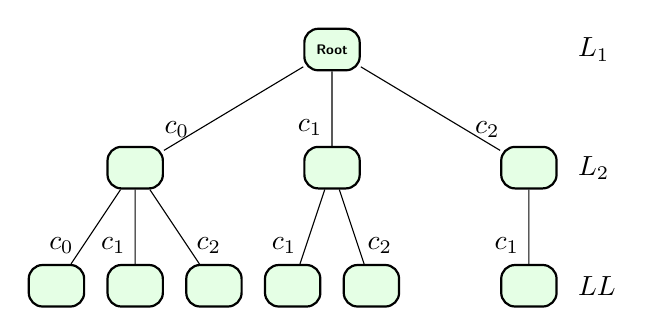
\begin{tikzpicture}[>=stealth',
level 1/.style={sibling distance = 2.5cm},
level 2/.style={sibling distance = 1cm},
level distance = 1.5cm]
\node (R) [node1] {\tiny Root}
	child { node [node1] {} 
		child { node [node1] {} edge from parent node [near end, left] {$c_0$}}
		child { node [node1] {} edge from parent node [near end, left] {$c_1$}}
		child { node [node1] {} edge from parent node [near end, right] {$c_2$}}
		edge from parent node [near end, left] {$c_0$}	
	}
	child { node [node1] {}
		child { node [node1] {} edge from parent node [near end, left] {$c_1$}}
		child { node [node1] {} edge from parent node [near end, right] {$c_2$}}
		edge from parent node [near end, left] {$c_1$}
	}
	child { node [node1] {} 
		child { node [node1] {} edge from parent node [near end, left] {$c_1$}}
		edge from parent node [near end, right] {$c_2$} 
};	
%----------------- Level labels --------------	
	\begin{scope}[every node/.style={right}]
		\path (R 				-| R-3-1) ++(5mm,0) node {$L_1$};
		\path (R-3 			-| R-3-1) ++(5mm,0) node {$L_2$};
		\path (R-3-1		-| R-3-1) ++(5mm,0) node {$LL$};
	\end{scope}			
\end{tikzpicture}
\caption{Example of multiset-trie structure \DIFaddbeginFL \DIFaddFL{containing multisets multisets $\emptyset, \{ 1,1,2 \},$ $\{ 1,2,2 \},$ $\{ 2 \},$ $\{ 1,2 \},$ $\{ 2,2 \}$}\DIFaddendFL . \DIFaddbeginFL \DIFaddFL{The }\emph{\DIFaddFL{Null}} \DIFaddFL{children are omitted.}\DIFaddendFL }
\label{fig:sketch}
\end{figure}

Let a pair $(L_i, c_j)$ represents a node with label $c_j$ at a level $L_i.$ 
The pair $(L_1,c_j)$ is equivalent to $(L_1,root),$ since the first level has 
the root node only. According to Figure~\ref{fig:sketch} we can extract 
inserted multisets as follows:

\begin{eqnarray*}
(L_1,root) \rightarrow (L_2,c_0) \rightarrow (LL,c_0) & = & \{ 1^0, 2^0 \} = \emptyset \\
(L_1,root) \rightarrow (L_2,c_0) \rightarrow (LL,c_1) & = & \{ 1^0, 2^1 \} = \{ 2 \} \\
(L_1,root) \rightarrow (L_2,c_0) \rightarrow (LL,c_2) & = & \{ 1^0, 2^2 \} = \{ 2,2 \} \\
(L_1,root) \rightarrow (L_2,c_1) \rightarrow (LL,c_1) & = & \{ 1^1, 2^1 \} = \{ 1,2 \} \\
(L_1,root) \rightarrow (L_2,c_1) \rightarrow (LL,c_2) & = & \{ 1^1, 2^2 \} = \{ 1,2,2 \} \\
(L_1,root) \rightarrow (L_2,c_2) \rightarrow (LL,c_1) & = & \{ 1^2, 2^1 \} = \{ 1,1,2 \} 
\end{eqnarray*}
where $e^k$ represents an element $e$ with multiplicity $k.$
% section 3
\section{Multiset-trie operations} \label{c:operations}

%
Let $\mathcal{M}$ be a multiset-trie and let $M$ be a set of multisets that are 
inserted into the multiset-trie $\mathcal{M}.$ We define a type \emph{Multiset} in 
order to use it as a representation of a multiset. The type \emph{Multiset} is 
an array $m$ of constant length $\sigma,$ where $i$-th cell represents the element 
$\phi^{-1}(i)$ from $\Sigma$ with multiplicity $m[i].$ From now on\DIFaddbegin \DIFadd{, }\DIFaddend we 
agree that the first cell of an array has index 1. Let us have an example of a 
\emph{Multiset} instance with $\sigma = 2:$
%
\begin{center}
\begin{tabular}{ccc}
Multiset & & Instance of type Multiset \\
$\{ 1,1,2 \}$ & $\cong $ & 
\begin{tabular}{|c|c|}
\hline 
2 & 1 \\
\hline 
\multicolumn{1}{c}{\tiny 1} & \multicolumn{1}{c}{\tiny 2} \\
\end{tabular}
\end{tabular}
\end{center}
%
The operations supported by the multiset-trie data structure are as follows.
%
\begin{enumerate}
\item \textsc{insert}($\mathcal{M}$, $m$): inserts a multiset $m$ into 
$\mathcal{M}$ if $m\not\in M;$
%
\item \textsc{search}($\mathcal{M}$, $m$): returns true if a multiset $m\in M$ 
for a given $\mathcal{M},$ and returns false otherwise;
%
\item \textsc{delete}($\mathcal{M}$, $m$): returns true if a multiset $m$ was 
successfully deleted from $\mathcal{M},$ and returns false otherwise (in case 
$m\not\in M$);
%
\item \textsc{submsetExistence}($\mathcal{M}$, $m$, $dev$): returns true if 
there exists a $x\in M$ for a given $\mathcal{M}$ such that $x\subseteq m$ 
and $| x[i] - m[i] |\leq dev$ for $1\leq i\leq \sigma$, and returns false otherwise; 
%
\item \textsc{supermsetExistence}($\mathcal{M}$, $m$, $dev$): returns true if 
there exists a $x\in M$ for a given $\mathcal{M}$ such that $x\supseteq m$ 
and $| x[i] - m[i] |\leq dev$ for $1\leq i\leq \sigma$, and returns false otherwise; 
%
\item \textsc{getAllSubmsets}($\mathcal{M}$, $m$, $dev$): returns the set of multisets 
$\{ x \in M : x\subseteq m \wedge |x[i]-m[i]|\leq dev \}$ for a given 
$\mathcal{M},$ where $1\leq i\leq \sigma;$
%
\item \textsc{getAllSupermsets}($\mathcal{M}$, $m$, $dev$): returns the set of multisets 
$\{ x\in M : x\supseteq m \wedge |x[i]-m[i]|\leq dev \}$ for a given $\mathcal{M},$
where $1\leq i\leq \sigma.$
%
\end{enumerate}

In the following subsections\DIFaddbegin \DIFadd{, }\DIFaddend we will present each operation of the multiset-trie 
data structure separately. 

Firstly we would like to describe some notations that will be used. The 
multiset-trie data structure is a recursive data structure. Hence, any \DIFdelbegin \DIFdel{sub 
tree }\DIFdelend \DIFaddbegin \DIFadd{subtree 
}\DIFaddend of a multiset-trie $\mathcal{M}$ is again a multiset-trie. This fact allows 
us to use the root node of a multiset-trie as its representative. Thus, the notation 
$\mathcal{M}$ will be used instead of $\mathcal{M}.root$ to refer to the root 
node of $\mathcal{M}.$ Non-existing or \emph{Null} nodes in multiset-trie will 
be marked as \emph{Null} and existing nodes at the level $LL$ will be marked 
as \emph{accepting} nodes. The array slicing operation will be used as follows. 
For a given array $a,$ $a[i:]$ represents the array obtained from $a$ by taking 
only the cells from index $i$ until the last cell. 


\subsection{Insert} \label{s:insert}
The procedure \textsc{insert}($\mathcal{M}$, $m$) inserts a new instance $m$ of 
type Multiset into multiset-trie $\mathcal{M}$. If the complete path already 
exists, then \DIFaddbegin \DIFadd{the }\DIFaddend procedure leaves the structure unchanged. Otherwise\DIFaddbegin \DIFadd{, }\DIFaddend it extends 
partially existing or creates a new complete path. The procedure does not return 
any result. The pseudocode for procedure \textsc{insert} is presented in 
Algorithm~\ref{alg:insert}.


\begin{algorithm}[h!]
\caption{Procedure \textsc{insert}}
\label{alg:insert}
\begin{algorithmic}[1]
\Procedure{\textsc{insert}}{$\mathcal{M}$, $m$}
\State $currentNode \gets \mathcal{M}$
\For{$i=1$ to $\sigma$}
\If {child $c_{m[i]}$ of $currentNode$ is \emph{Null}}
\State create new child $c_{m[i]}$ of $currentNode$
\EndIf
\State $currentNode \gets c_{m[i]}$
\EndFor
\State mark $currentNode$ as \emph{accepting}
\EndProcedure
\end{algorithmic}
\end{algorithm}

\subsection{Search}\label{s:search}
The function \textsc{search}($\mathcal{M}$, $m$) checks if the complete path corresponding to 
a given multiset $m$ exists in the structure $\mathcal{M}.$ The function returns 
true if the multiset $m$ exists in $\mathcal{M}$, and returns false otherwise. The 
function \textsc{search} is presented in Algorithm~\ref{alg:search}.

\begin{algorithm}[h!]
\caption{Function \textsc{search}}
\label{alg:search}
\begin{algorithmic}[1]
\Function{\textsc{search}}{$\mathcal{M}$, $m$}
\State $currentNode \gets \mathcal{M}$
\For{$i=1$ to $\sigma$}
\If {child $c_{m[i]}$ of $currentNode$ is \emph{Null}}
\State \Return False
\EndIf
\State $currentNode \gets c_{m[i]}$
\EndFor
\State \Return True
\EndFunction
\end{algorithmic}
\end{algorithm}

\subsection{Delete} \label{s:delete}
\DIFdelbegin \DIFdel{The function }\DIFdelend \DIFaddbegin \DIFadd{Function }\DIFaddend \textsc{delete}($\mathcal{M},$ $m$) searches for the complete path 
that corresponds to $m$ in order to remove it. If the path can not be found, the 
function immediately returns false. During \DIFaddbegin \DIFadd{the }\DIFaddend search, the function keeps track of the 
number of children for every node. It marks the nodes that have more than one child 
as \emph{parent nodes} and remembers the label of the child\DIFaddbegin \DIFadd{, }\DIFaddend which is a potential node 
where the sub-tree will be cut to remove the multiset. The parent node is needed to 
perform a removal \DIFdelbegin \DIFdel{, }\DIFdelend because the multiset-tire is an explicit data structure. When \DIFaddbegin \DIFadd{the }\DIFaddend search 
is completed, the function removes the sub-tree of the last found parent node \DIFdelbegin \DIFdel{, }\DIFdelend and 
returns true. In such a way\DIFdelbegin \DIFdel{after deletion }\DIFdelend \DIFaddbegin \DIFadd{, after deletion, }\DIFaddend all the prefixes for other multisets are 
preserved in $\mathcal{M}$ and $m$ is removed. The function \textsc{delete} is 
presented in Algorithm~\ref{alg:delete}.


\begin{algorithm}[h!]
\caption{Function \textsc{delete}}
\label{alg:delete}
\begin{algorithmic}[1]
\Function{\textsc{delete}}{$\mathcal{M},$ $m$}
\State $currentNode \gets \mathcal{M}$
\State $parent \gets currentNode$ 
\State $position \gets 1$
\For {$i=1$ to $\sigma$}
\If {child $c_{m[i]}$ of $currentNode$ is \emph{Null}}
\State \Return False
\EndIf
\State $numChildren \gets 0$
\For {$j=0$ to $n-1$}
\If {child $c_j$ of $currentNode$ is not \emph{Null}}
\State $numChildren\gets numChildren+1$
\EndIf
\EndFor
\If {$numChildren$ is not $1$}
\State $parent\gets currentNode$
\State $position \gets i$
\EndIf
\State $currentNode \gets c_{m[i]}$
\EndFor
\State child $c_{m[position]}$ of $parent\gets$ \emph{Null}
\State \Return True
\EndFunction
\end{algorithmic}
\end{algorithm}

\subsection{Sub-multiset existence} \label{s:subexists}
The function \textsc{submsetExistence}($\mathcal{M},m,dev$) checks if there exists 
a multiset $x$ in $\mathcal{M},$ that satisfies the condition $x\subseteq m$ and 
$| x[i] - m[i] | \leq dev,$ where $1\leq i \leq \sigma.$ 
The function starts with searching for an exact match $x=m$ in $\mathcal{M},$ 
since $m\subseteq m$ by definition of \DIFdelbegin \DIFdel{submultiset }\DIFdelend \DIFaddbegin \DIFadd{sub-multiset }\DIFaddend inclusion. If an exact match is 
not found in $\mathcal{M},$ the function uses multiset-trie to find the closest 
(the largest) \DIFdelbegin \DIFdel{submultiset }\DIFdelend \DIFaddbegin \DIFadd{sub-multiset }\DIFaddend of $m$ in $\mathcal{M}$ by decreasing \DIFaddbegin \DIFadd{the }\DIFaddend multiplicity of 
elements in $m.$ The parameter $dev$ is used to limit a maximal deviation of 
multiplicity for a particular element in $x$ with respect to $m.$ 
At every level\DIFaddbegin \DIFadd{, }\DIFaddend the function tries to proceed with the largest possible multiplicity of 
an element that is provided by $m.$ However, when the function reaches some level 
where it meets a \emph{Null} node and can not go further using \DIFaddbegin \DIFadd{the }\DIFaddend path provided by 
$m,$ it decreases the multiplicity of an element 
that corresponds to a current level with respect to the specified maximal deviation. 
Thus, the function can decrease \DIFaddbegin \DIFadd{the }\DIFaddend multiplicity of an element or eventually skip it in 
order to find the closest $x\subseteq m.$ The function \textsc{submsetExistence} 
is presented in Algorithm~\ref{alg:subexists}.

\begin{algorithm}[h!]
\caption{Function \textsc{submsetExistence}}
\label{alg:subexists}
\begin{algorithmic}[1]
\Function{\textsc{submsetExistence}}{$\mathcal{M}, m, dev$}
\State $currentNode \gets \mathcal{M}$
\If {$currentNode$ is \emph{accepting}}
\State \Return True
\EndIf
\For {$i=m[1]$ down to max($0, m[1]-dev$)}
\If {child $c_i$ of $currentNode$ is not \emph{Null}}
\If {\textsc{submsetExistence}($c_i,m[2:], dev$)}
\State \Return True
\EndIf
\EndIf
\EndFor
\State \Return False
\EndFunction
\end{algorithmic}
\end{algorithm}

\subsection{Super-multiset existence} \label{s:superexists}
The function \textsc{supermsetExistence}($\mathcal{M},m,dev$) checks if there 
exists \DIFdelbegin \DIFdel{supermultiset }\DIFdelend \DIFaddbegin \DIFadd{super-multiset }\DIFaddend $x$ of a given multiset $m$ in $\mathcal{M},$ such that 
condition $| x[i] - m[i] |\leq dev$ is satisfied, where $1\leq i \leq \sigma.$ By analogy 
to the function \textsc{submsetExistence}, the function \textsc{supermsetExistence} 
starts by searching for an exact match $x=m$ in $\mathcal{M}.$ If an exact 
match is not found in $\mathcal{M},$ the function searches for the closest (the 
smallest) \DIFdelbegin \DIFdel{supermultiset }\DIFdelend \DIFaddbegin \DIFadd{super-multiset }\DIFaddend $x$ of $m$ in $\mathcal{M}$ by increasing multiplicity 
of elements in $m.$ At every level\DIFaddbegin \DIFadd{, }\DIFaddend the function tries to proceed with the smallest 
possible multiplicity of an element that is provided by $m.$ However, when \DIFaddbegin \DIFadd{the }\DIFaddend function 
reaches some level where it meets a \emph{Null} node and can not go further using 
\DIFaddbegin \DIFadd{the }\DIFaddend path provided by $m,$ it increases the multiplicity of an element that corresponds to a 
current level according to the deviation parameter $dev.$ Thus, the function \textsc{supermsetExistence} 
can increase multiplicity of an element up to $n-1,$ where $n$ is the degree of 
a node in $\mathcal{M},$ to find the closest \DIFdelbegin \DIFdel{supermultiset }\DIFdelend \DIFaddbegin \DIFadd{super-multiset }\DIFaddend $x\supseteq m$ in 
$\mathcal{M}.$ The function \textsc{supermsetExistence} is presented in 
Algorithm~\ref{alg:superxists}.


\begin{algorithm}[h!]
\caption{Function \textsc{supermsetExistence}}
\label{alg:superxists}
\begin{algorithmic}[1]
\Function{\textsc{supermsetExistence}}{$\mathcal{M},m,dev$}
\State $currentNode \gets \mathcal{M}$
\If {$currentNode$ is \emph{accepting} }
\State \Return True
\EndIf
\For {$i=m[1]$ to min($n-1, m[1] + dev$)}
\If {child $c_i$ of $currentNode$ is not \emph{Null}}
\If {\textsc{supermsetExistence}($c_i,$ $m[2:], dev$)}
\State \Return True
\EndIf
\EndIf
\EndFor
\State \Return False
\EndFunction
\end{algorithmic}
\end{algorithm}


\subsection{Get all sub-multisets and get all super-multisets} \label{s:getall}
The algorithms for functions \textsc{getAllSubmsets} and 
\textsc{getAllSupermsets} are based entirely on algorithms for 
\textsc{submsetExistence} and \textsc{supermsetExistence} functions that do not 
terminate on the first existing sub/\DIFdelbegin \DIFdel{supermultiset}\DIFdelend \DIFaddbegin \DIFadd{super-multiset}\DIFaddend , but store the results and 
continue \DIFaddbegin \DIFadd{the }\DIFaddend procedure until all existing sub/\DIFdelbegin \DIFdel{supermultisets }\DIFdelend \DIFaddbegin \DIFadd{super-multisets }\DIFaddend in $\mathcal{M}$ are 
found and stored. The functions \textsc{getAllSubmsets} and \textsc{getAllSupermsets} 
are presented in Algorithm~\ref{alg:getallsub} and Algorithm~\ref{alg:getallsup} respectively.

In order to record a multiset during multiset-trie traversal\DIFaddbegin \DIFadd{, }\DIFaddend we use the variable $x$ in the algorithms.
It is an empty array of size $\sigma$ where we store multiplicities of elements at 
each level as we traverse the tree. The variable $result$ is used as a container for storing 
\DIFdelbegin \DIFdel{submultisets }\DIFdelend \DIFaddbegin \DIFadd{sub-multisets }\DIFaddend of $m$ found during traversal. Both variables $x$ and $result$ are presented 
as global, however\DIFaddbegin \DIFadd{, }\DIFaddend they could be passed to the recursive function as parameters.

\begin{algorithm}[h!]
\caption{Function \textsc{getAllSubmsets}}
\label{alg:getallsub}
\begin{algorithmic}[1]
\State $result \gets$ empty container
\State $x \gets$ empty array of size $\sigma$
\Function{\textsc{getAllSubmsets}}{$\mathcal{M}, m, dev$}
\State $currentNode \gets \mathcal{M}$
\If {$currentNode$ is \emph{accepting}}
\State add copy of $x$ to $result$ 
\EndIf
\For {$i=m[1]$ down to max($0, m[1]-dev$)}
\If {child $c_i$ of $currentNode$ is not \emph{Null}}
\State $x[1]\gets i$
\State \textsc{getAllSubmsets}($c_i,m[2:], dev$)
\EndIf
\EndFor
\EndFunction
\end{algorithmic}
\end{algorithm}


\begin{algorithm}[h!]
\caption{Function \textsc{getAllSupermsets}}
\label{alg:getallsup}
\begin{algorithmic}[1]
\State $result \gets$ empty container
\State $x \gets$ empty array of size $\sigma$
\Function{\textsc{getAllSupermsets}}{$\mathcal{M},m,dev$}
\State $currentNode \gets \mathcal{M}$
\If {$currentNode$ is \emph{accepting} }
\State add copy of $x$ to $result$ 
\EndIf
\For {$i=m[1]$ to min($n-1, m[1] + dev$)}
\If {child $c_i$ of $currentNode$ is not \emph{Null}}
\State $x[1]\gets i$
\textsc{getAllSupermsets}($c_i,$ $m[2:], dev$)
\EndIf
\EndFor
\EndFunction
\end{algorithmic}
\end{algorithm}
% section 4
\section{Mathematical analysis of the structure} \label{c:analysis}
%
In this chapter\DIFaddbegin \DIFadd{, }\DIFaddend we present theoretical results of time and space complexity of
the multiset-trie data structure. In the following Section~\ref{s:timecomplexity} 
we discuss the running time complexity of the presented algorithms. First, in 
Section~\ref{ss:mathmodel}, we present \DIFdelbegin \DIFdel{our }\DIFdelend \DIFaddbegin \DIFadd{the }\DIFaddend mathematical model that we use 
to describe the distribution of multisets in the multiset-trie and input data. 
Using \DIFaddbegin \DIFadd{a }\DIFaddend probabilistic approach and tools from a Galton-Watson process\DIFaddbegin \DIFadd{, }\DIFaddend we 
measure the expected cardinality of the multiset-trie in Theorem~\ref{thm:exp_nodes}. 
Further, we derive the expected cardinality of the searched subtree of the 
multiset-trie parametrized by an input multiset in Corollary~\ref{cor:exp_nodes_param}.

In Section~\ref{ss:getall} we discuss the running time complexity of the functions 
\textsc{getAllSubmsets} and \textsc{getAllSupermsets}. We observe that the 
complexity of functions is exponential. Moreover, the \DIFdelbegin \DIFdel{worst case }\DIFdelend \DIFaddbegin \DIFadd{worst-case }\DIFaddend running time 
complexity is the same for both functions\DIFaddbegin \DIFadd{, }\DIFaddend and its upper bound is the cardinality of 
the multiset-trie.

The remaining "existence" functions are discussed in the Section~\ref{ss:exists}. 
We observe that out of \DIFaddbegin \DIFadd{the }\DIFaddend scope of our mathematical model\DIFaddbegin \DIFadd{, }\DIFaddend unlike in functions 
\textsc{getAllSubmsets} and \textsc{getAllSupermsets} the mapping $\phi$ has an 
impact on performance of the functions \textsc{submsetExistence} and 
\textsc{supermsetExistence}. In particular, the frequency analysis of the symbols 
from $\Sigma$ in input data determines such a $\phi$ that gives a boost in performance. 

We find that the performance of the functions \textsc{submsetExistence} and 
\textsc{supermsetExistence} in the \DIFdelbegin \DIFdel{worst case }\DIFdelend \DIFaddbegin \DIFadd{worst-case }\DIFaddend scenario is also exponential and 
does not depend on the outcome of the functions. We give a quite precise upper 
bound for the \DIFdelbegin \DIFdel{worst case }\DIFdelend \DIFaddbegin \DIFadd{worst-case }\DIFaddend running time complexity, which appears to be the same 
for both functions. However, it must be stressed that for the positive outcome\DIFaddbegin \DIFadd{, }\DIFaddend an 
exponential behavior holds only on specific cases, such as \DIFaddbegin \DIFadd{the }\DIFaddend presence of the \DIFdelbegin \DIFdel{emptyset 
}\DIFdelend \DIFaddbegin \DIFadd{empty set 
}\DIFaddend in the multiset-trie. 

Finalizing the mathematical analysis, we present the study of space complexity 
of the multiset-trie in \DIFdelbegin \DIFdel{the }\DIFdelend Section~\ref{s:spacecomplexity}. We show that the space 
used for the storage is asymptotically equal to the size of the input data. 

\subsection{Time complexity of the algorithms}\label{s:timecomplexity}
The performance of the functions will be measured by the number of 
visited nodes in a multiset-trie during \DIFaddbegin \DIFadd{the }\DIFaddend execution of a particular query by the 
functions \textsc{search}, \textsc{delete}, \textsc{submsetExistence}, 
\textsc{supermsetExistence}, \textsc{getAllSubmsets}, \textsc{getAllSupermsets} 
and the procedure \textsc{insert}.
%

By the design of the multiset-trie, it is easy to see that the functions \textsc{search},
\textsc{delete} and the procedure \textsc{insert} have complexity of $O(\sigma).$
Because $\sigma$ is defined when the structure is initialized and does not depend
on the user input afterwards, the asymptotic complexity of the functions \textsc{search}, 
\textsc{delete} and the procedure \textsc{insert} is $O(1).$ Nonetheless, in the general 
case\DIFaddbegin \DIFadd{, }\DIFaddend the complexity is $O(\sigma).$

In what follows, we focus on \DIFaddbegin \DIFadd{the }\DIFaddend analysis of the more involved functions:
\textsc{submsetExistence}, \textsc{supermsetExistence}, \textsc{getAllSubmsets}
and \textsc{getAllSupermsets}.

\subsubsection{Mathematical model} \label{ss:mathmodel}
We start with the basics of our mathematical model. Let $\Sigma$ be an alphabet of
cardinality $\sigma,$ such that $\Sigma = \{ 1,2, \ldots, \sigma \}.$ Define $N$
to be the set of all possible multisets that can be inserted in \DIFaddbegin \DIFadd{a
}\DIFaddend multiset-trie. Let $n$ be the maximal degree of a node in \DIFaddbegin \DIFadd{a }\DIFaddend multiset-trie.
Then the maximal multiplicity of an element in a multiset is equal to $n-1.$
Thus, the number of multisets in a complete multiset-trie is $ |N| = n^{\sigma}.$
%
Let $M$ be a collection of multisets inserted into multiset-trie $\mathcal{M}.$
All the multisets in $M$ are constructed from the alphabet $\Sigma$ according
to the parameters $\sigma$ and $n$. Hence, any multiset $m\in M,$ 
has at most $\sigma$ distinct elements that are members of $\Sigma$ and 
every distinct element in $m$ has multiplicity strictly less than $n.$
%
Because a multiset does not distinguish different orderings, it is assumed, for
simplicity\DIFaddbegin \DIFadd{, }\DIFaddend that all elements are ordered in \DIFdelbegin \DIFdel{an }\DIFdelend ascending order. A multiset $m$ is
represented as $\{1^{k_1},2^{k_2},\ldots, \sigma^{k_\sigma}\},$ where $e^{k_e}$
represents an element $e\in\Sigma$ with multiplicity $k_e.$
%

Denote the nodes of multiset-trie on all levels but on $\sigma + 1$ as \emph{internal}
and nodes on leaf level as \emph{leaf} nodes.
%
Observe that every internal non-root node has a degree at least~1. Indeed an
insertion of a multiset requires \DIFdelbegin \DIFdel{a }\DIFdelend construction of a path of length~$\sigma + 1,$
meaning that if an internal node exists in a multiset-trie\DIFaddbegin \DIFadd{, }\DIFaddend it must have a degree
at least~1. It also follows that the height of a multiset-trie is always~$\sigma +1$
as soon as at least one multiset is inserted into the data structure.

Our model assumes that all the inserted multisets are chosen with the same probability,
meaning that for some $p\in (0,1)$\DIFaddbegin \DIFadd{, }\DIFaddend the following holds:
\[
P(m\in M) = p, \quad \forall~m\in N.
\]
%
Let $\xi_1, \xi_2, \ldots, \xi_{\sigma+1}$ be random variables such that $\xi_i$
represents the number of nodes in a multiset-trie on $i$-th level. For every node $j$ 
on $i$-th level we assign a random variable $\xi_{ij}$ to be the number of its children, 
such that $j\in[1,\xi_i].$ Then for every $i\in[1,\sigma]$ the following holds:
%
\begin{equation}\label{eq:sum_recursive}
\xi_{i+1} = \sum_{j=1}^{\xi_i} \xi_{ij},
\end{equation}
%
where $\xi_1 = 1.$
%
It is easy to see that the variable $\xi_{i+1}$ can have values in the interval
$[\xi_i,n^{i}]$ and the value of the variable $\xi_{ij}$ is within the interval $[1,n].$
Without conditioning on the existence of any node in multiset-trie, 
it is easy to describe the probability of \DIFaddbegin \DIFadd{the }\DIFaddend existence of any individual node.

\begin{lemma}\label{l:prob-node-existence}
Any potential node on a fixed level $i,$ where $i\in \{ 1,2,\ldots, \sigma +1 \}$ exists, %independently of others,
with probability
\begin{equation}
p_i=1-(1-p)^{n^{\sigma + 1 -i}}.
\end{equation}
\end{lemma}
\begin{proof}
Let $v$ be an arbitrary node in a multiset-trie on an arbitrary level $i.$ Consider
the subtree with the root $v$ and call it $v$-subtree. Since the height of the
multiset-trie is $\sigma + 1$ we can calculate the height of the $v$-subtree.
Taking \DIFdelbegin \DIFdel{in }\DIFdelend \DIFaddbegin \DIFadd{into }\DIFaddend account that the root node has height 1, the height of the $v$-subtree is
%
\[
h_v = \sigma + 1 - i.
\]
%
A node in a multiset-trie exists if at least one node exists on the leaf level of its
subtree, i.e. a node on the level $\sigma + 1$ that belongs to $v$-subtree. The possible
number of nodes on the leaf level of $v$-subtree can be easily calculated knowing its height.
It is equal to
%
\[
n^{\sigma + 1 - i}.
\]
%
A node at level $\sigma+1$ exists with probability $p,$ where $p = P(m\in M).$
Thus, the probability that there are no nodes on leaf level in $v$-subtree is
%
\[
(1-p)^{n^{\sigma +1 - i}}.
\]
%
The claim follows by taking the complement probability of the above result. 

%
\end{proof}

However, in order to determine the distribution of $\xi_{ij}$, one needs a lemma of a different kind.

\begin{lemma}\label{l:prob-children}
Suppose that a node $v$ exists at level $1\leq i\leq\sigma$.
Then the number of its children $\xi_{iv}$ is modeled by a zero-truncated binomially
distributed random variable on parameters $n$ and $p_{i+1}$. In particular,
the probability of node $v$ having $k$ children equals to
\begin{equation}\label{eq:pdf}
P(\xi_{iv} = k) = \frac{\binom{n}{k} (1-p_{i+1})^{n-k}}{1-(1-p_{i+1})^n}
\end{equation}
and the corresponding probability generating function equals to
\begin{equation}\label{eq:generating_func}
G_i(z) = \frac{(1+p_{i+1}(z-1))^n - (1-p_{i+1})^n}{1-(1-p_{i+1})^n}.
\end{equation}
\end{lemma}
\begin{proof}
In order to prove the lemma, we have to show that
$\xi_{iv}\sim\mathcal{B}_0(n, p_{i+1}).$
Consider an arbitrary node $v$ on level $1\leq i\leq\sigma.$ According to the
definition of the multiset-trie\DIFaddbegin \DIFadd{, }\DIFaddend a node exists at level $i$ if and only if
it has at least one child. Note that this is not true for the nodes on the leaf
level $\sigma + 1.$ Implies, a node on level $i$ can have
$k\in\{ 1,2,\ldots, n\}$ children. Let $X_0, X_1, \ldots, X_{n-1}$ be random
variables, they are defined as follows:
\[
X_k = \begin{cases}
0 & \textrm{child $k$ of node $v$ does not exist} \\
1 & \textrm{child $k$ of node $v$ exists} \\
\end{cases}
\]
As it was shown in previous Lemma~\ref{l:prob-children}, the distribution of 
$X_k$ is $X_k\sim Bernoulli(p_{i+1}).$ Since our model assumes that all the 
multisets in $M$ are chosen uniformly at random, the variables 
$X_k,X_l$ are independent for $k\neq l.$ But in our case the node $v$ can not 
have 0 children, so the sum $\sum_{k=1}^n X_k$ has a zero-truncated binomial 
distribution:
%
\[
\sum_{k=1}^n X_k \sim\mathcal{B}_0(n,p_{i+1})
\]
%
which completes the proof.

\end{proof}
%
Knowing the probability density and probability generating functions of $\xi_{ij}$ 
from Lemma~\ref{l:prob-children}, we \DIFdelbegin \DIFdel{now can }\DIFdelend \DIFaddbegin \DIFadd{can now }\DIFaddend estimate the number of nodes in 
a randomly generated multiset-trie as follows:
%
\begin{equation}\label{eq:num_nodes}
\mathbb{E}( | \mathcal{M} | ) = \mathbb{E}\left[ \sum_{i=1}^{\sigma+1} \xi_i \right].
\end{equation}
%

%Note that in a real world models multisets in $M$ are not chosen with the same 
%probability. Specifically, in some cases, the probability $P(m\in M)$ varies 
%dramatically and can be even equal to $0.$ For example, if words are mapped 
%to multisets, then the sample space $N$ contains very large multisets. However, 
%most of them will have probability $P(m\in M)=0,$ because a word that would correspond 
%to such a multiset simply does not exist. So, we can safely conclude that multiset-trie 
%is an input sensitive data structure, because the size of multiset-trie $|\mathcal{M}|$ 
%depends on the probability distribution function $P(m\in M).$
%

In order to evaluate~(\cref{eq:num_nodes}) we will use some of the tools from 
a Galton-Watson process, see Gardiner~\cite{gardiner1985stochastic} for 
an introduction.
Using the equations~(\cref{eq:sum_recursive}) and~(\cref{eq:generating_func}) we can 
derive the probability generating function for the random variable $\xi_{i+1}$ as 
\begin{equation}\label{eq:g_rec}
G_{\xi_{i+1}}(z) = G_{\xi_i}(G_i(z)).
\end{equation}
Since there is always precisely one node at the \DIFdelbegin \DIFdel{root-level}\DIFdelend \DIFaddbegin \DIFadd{root level}\DIFaddend , we have $P(\xi_1 = 1) = 1.$ 
Hence, the probability generating function for the random variable $\xi_1$ is 
\begin{equation}\label{eq:g_xi_one}
G_{\xi_1}(z) = z^1 = z
\end{equation}
which is the initial condition for the recursive equation~(\cref{eq:g_rec}).

\begin{proposition}\label{prop:exp_rec}
The expectation of the random variable $\xi_{i+1}$ can be expressed 
as follows.
\[
\mathbb{E}(\xi_{i+1}) = \mathbb{E}(\xi_i)\mathbb{E}(\mathcal{B}_0(n,p_{i+1}))
\]
for $1\leq i\leq\sigma.$
\end{proposition}
\begin{proof}
Using the following property of probability generating function
\begin{equation}\label{eq:prop_exp-pgf}
G_X'(1^-) = \mathbb{E}(X)
\end{equation}
the expectation for the random variable $\xi_{i+1}$ can be derived in terms of 
the equation~(\cref{eq:g_rec}).
\begin{eqnarray}\label{eq:exp}
\mathbb{E}(\xi_{i+1}) &=& G_{\xi_{i+1}}'(1^-) \nonumber \\
&=& G_{\xi_i}'(G_i(1^-))G_i'(1^-).
\end{eqnarray}
According to~(\cref{eq:pdf}) and~(\cref{eq:generating_func}) the value of $G_i(z)$ at 
$1$ is $1$ and the value of its derivative at $1$ is $\mathbb{E}(\mathcal{B}_0(n,p_{i+1})).$ 
Substituting the values of $G_i(1^-)$ and $G_i'(1^-),$ and applying the 
property~(\cref{eq:prop_exp-pgf}) we complete the proof.

\end{proof}
%
From the Proposition~\ref{prop:exp_rec} above and Lemma~\ref{l:prob-children} we 
can conclude that 
\begin{eqnarray}
\mathbb{E}(\xi_{i}) &=& \mathbb{E}(\xi_{i-1})\mathbb{E}\left( \mathcal{B}_0(n,p_{i}) \right) \nonumber \\
& = & \mathbb{E}(\xi_{i-1})\frac{np_{i}}{1-(1-p_{i})^n}.
\end{eqnarray}

\begin{theorem}\label{thm:exp_level}
Let $\mathcal{M}$ be a multiset-trie defined with parameters $n,$ $\sigma,$ and denote the number 
of nodes on every level $i$ by a random variable $\xi_i.$ Furthermore, let all multisets appear in 
$\mathcal{M}$ with equal probability $p\in (0,1).$ Then the expected number 
of nodes on every level of $\mathcal{M},$ i.e. $\mathbb{E}(\xi_i)$ is defined as 
\begin{equation}\label{eq:nodes_level}
\mathbb{E}(\xi_{i}) = n^{i-1} \frac{1-(1-p)^{n^{\sigma +1 -i}}}{1-(1-p)^{n^{\sigma}}}.
\end{equation}
\end{theorem}
\begin{proof}
According to~(\cref{eq:g_xi_one}) the expected number of nodes on the first level is 1. \\
Using $\mathbb{E}(\xi_1) = 1$ and the result from Proposition~\ref{prop:exp_rec}
we get
\begin{eqnarray*}
\mathbb{E}(\xi_{i}) &=& \prod_{j=2}^{i} \frac{n p_j}{1-(1-p_j)^n}
= \prod_{j=2}^{i} n \frac{1-(1-p)^{n^{\sigma +1-j}}}{1-(1-p)^{n^{\sigma + 2 -j}}} \\
&=& n^{i-1} \frac{1-(1-p)^{n^{\sigma +1 -i}}}{1-(1-p)^{n^{\sigma}}}
\end{eqnarray*}

\end{proof}

Having derived the expected number of nodes on every level of multiset-trie, the
expected value of the total number of nodes in a multiset-trie can be calculated 
with respect to the parameters $n,$ $\sigma$ and $p.$ This result is obtained in 
the next theorem.

\begin{theorem}\label{thm:exp_nodes}
The expected cardinality of a multiset-trie defined on parameters $n,$ $\sigma$ 
and $p$ can be computed as 
\begin{equation}
\mathbb{E}( | \mathcal{M} | ) = \sum_{i=1}^{\sigma+1} n^{i-1} \frac{1-(1-p)^{n^{\sigma +1 -i}}}{1-(1-p)^{n^{\sigma}}},
\end{equation}
where $r = (1-p)^n,$ so $r\in(0,1).$
\end{theorem}
\begin{proof}
Using the results obtained from Theorem~\ref{thm:exp_level} we compute 
\begin{eqnarray*}
\mathbb{E}( | \mathcal{M} | ) &=& \mathbb{E}\left[ \sum_{i=1}^{\sigma+1} \xi_i \right] \\
&=& \sum_{i=1}^{\sigma + 1} n^{i-1} \frac{1-(1-p)^{n^{\sigma + 1 -i}}}{1-(1-p)^{n^{\sigma}}} \\
\end{eqnarray*}

\end{proof}

With the expected number of nodes in a multiset-trie $\mathcal{M}$ obtained from 
Theorem~\ref{thm:exp_nodes}, we can now generalize the result for a subtree 
in $\mathcal{M}$ parametrized by an input multiset $m.$ The subtrees that we 
are interested in are the ones that contain all the \DIFdelbegin \DIFdel{submultisets }\DIFdelend \DIFaddbegin \DIFadd{sub-multisets }\DIFaddend or all the 
\DIFdelbegin \DIFdel{supermultisets }\DIFdelend \DIFaddbegin \DIFadd{super-multisets }\DIFaddend of $m.$ In order to calculate the expected cardinality of such 
subtrees\DIFaddbegin \DIFadd{, }\DIFaddend we need the following definition. 

\begin{definition}\label{def:params}
Let $m = \{ 1^{k_1}, 2^{k_2}, \ldots, \sigma^{k_\sigma} \},$ where 
$e^{k_e}$ is an element $e$ with multiplicity $k_e.$ Let $M_1, M_2$ be 
the subsets of the set $M,$ such that $M_1 = \{ x\in M : x\subseteq m \}$ and 
$M_2 = \{ x\in M : x\supseteq m \}.$
Define $\alpha_i$ and $\beta_i$ as follows 
\begin{equation*}
\alpha_i = \begin{cases}
1, & i=0 \\
\prod_{j=1}^i (k_j+1), & 1\leq i\leq\sigma \\
\end{cases}
\end{equation*} 
and 
\begin{equation*}
\beta_i = \begin{cases}
1, & i=0 \\
\prod_{j=1}^i (n-k_j-1), & 1\leq i\leq\sigma \\
\end{cases}.
\end{equation*}
\end{definition}

The expected cardinality of the subtrees containing the multisets from $M_1$ or $M_2$ 
is defined in the following corollary.

\begin{corollary}\label{cor:exp_nodes_param}
Let $M_1, M_2, \alpha_i$ and $\beta_i$ be defined as in previous Definition~\ref{def:params}, 
then the expected cardinality of a multiset-trie subtree $\mathcal{M}_{M_1}$ that contains all the multisets 
from the set $M_1$ is equal to 
\begin{equation}\label{eq:nodes_sub_param}
\mathbb{E}( |\mathcal{M}_{M_1}| ) = \sum_{i=1}^{\sigma + 1} \alpha_{i-1} \frac{1-(1-p)^{\alpha_{i-1}}}{1-(1-p)^{\alpha_{\sigma}}}.
\end{equation}
The expected cardinality of a multiset-trie subtree $\mathcal{M}_{M_2}$ that contains all the multisets 
from the set $M_2$ is equal to 
\begin{equation}\label{eq:nodes_super_param}
\mathbb{E}( |\mathcal{M}_{M_2}| ) = \sum_{i=1}^{\sigma + 1} \beta_{i-1} \frac{1-(1-p)^{\beta_{i-1}}}{1-(1-p)^{\beta_{\sigma}}}.
\end{equation}
\end{corollary}
%
\begin{proof}
Using the results from Theorem~\ref{thm:exp_level} and Theorem~\ref{thm:exp_nodes} 
we derive the formulas~(\cref{eq:nodes_sub_param}) and~(\cref{eq:nodes_super_param}) 
by specifying the possible number of nodes on every level in the multiset-trie according 
to the multiset $m.$ Note that the formula~(\cref{eq:nodes_level}) assumes that on every 
level but the first one\DIFaddbegin \DIFadd{, }\DIFaddend there are $n$ possible nodes. Given \DIFdelbegin \DIFdel{submultiset or supermultiset 
}\DIFdelend \DIFaddbegin \DIFadd{sub-multiset or super-multiset 
}\DIFaddend query and an input multiset $m$ the number of nodes that will be traversed on level $i$ is 
defined by the number $k_{i-1}+1$ or $n-k_{i-1}-1$ for $i\geq 2.$ On level $i=1$ 
there is only one root node in any multiset-trie $\mathcal{M},$ which always exists 
if $M\neq\emptyset$ and is traversed for any type of query (\DIFdelbegin \DIFdel{submultiset and 
supermultiset}\DIFdelend \DIFaddbegin \DIFadd{sub-multiset and 
super-multiset}\DIFaddend ).

\end{proof}

\subsubsection{GetAllSubmsets and GetAllSupermsets}\label{ss:getall}
In this subsection we discuss the running time complexity of the functions 
\textsc{getAllSubmsets} and \textsc{getAllSupermsets}. It is obvious that any 
other algorithm for retrieving all the \DIFdelbegin \DIFdel{submultisets or supermultisets has worst 
case }\DIFdelend \DIFaddbegin \DIFadd{sub-multisets or super-multisets has worst-case
}\DIFaddend running time complexity \DIFaddbegin \DIFadd{of }\DIFaddend at least $O(|M|).$ Hence, the functions 
\textsc{getAllSubmsets} and \textsc{getAllSupermsets} have the \DIFdelbegin \DIFdel{worst case 
}\DIFdelend \DIFaddbegin \DIFadd{worst-case 
}\DIFaddend running time complexity $O(|\mathcal{M}|).$ Indeed, the case when the algorithms 
retrieve all the multisets stored in a multiset-trie by traversing the whole structure 
can be easily constructed. 

Consider the function \textsc{getAllSubmsets}. The function takes some multiset 
$m$ as an input argument. Then it returns a set of multisets $\{x\in M : x\subseteq m \}$ 
from the multiset-trie $\mathcal{M}$. Having a multiset $m$ set to the largest 
possible multiset in $N$ (it can also be larger) 
\[
m = \{ 1^{n-1},2^{n-1},\ldots, \sigma^{n-1} \}
\]
the whole multiset-trie is traversed during the \textsc{getAllSubmsets} query.

Now let us consider the function \textsc{getAllSupermsets}. Similarly, the function 
takes a multiset $m$ as an input argument. However, in this case\DIFaddbegin \DIFadd{, }\DIFaddend it returns the 
set of multisets $\{ x\in M : x\supseteq m \}$ from the multiset-trie 
$\mathcal{M}.$ In order to obtain a traversing of all the multiset-trie\DIFaddbegin \DIFadd{, }\DIFaddend one must set 
$m$ to the smallest possible multiset, i.e.\DIFaddbegin \DIFadd{, }\DIFaddend an empty multiset
\begin{equation*}
m = \{ \emptyset \} = \{ 1^0,2^0, \ldots, \sigma^0 \}.
\end{equation*}

Thus, we can conclude that the \DIFdelbegin \DIFdel{worst case }\DIFdelend \DIFaddbegin \DIFadd{worst-case }\DIFaddend running time complexity of the 
functions \textsc{getAllSubmsets} and \textsc{getAllSupermsets} is $O(\mathbb{E}( |\mathcal{M}| )).$ 
According to the Theorem~\ref{thm:exp_nodes} the expected number of visited 
nodes in the worst case is 
\begin{equation*}
O(\sum_{i=1}^{\sigma+1} n^{i-1} \frac{1-(1-p)^{n^{\sigma +1 -i}}}{1-(1-p)^{n^{\sigma}}}).
\end{equation*}
According to the Theorem~\ref{cor:exp_nodes_param} the \DIFdelbegin \DIFdel{worst case }\DIFdelend \DIFaddbegin \DIFadd{worst-case }\DIFaddend running 
time complexity given an input multiset $m$ for the function \textsc{getAllSubmsets} is 
\begin{equation*}
O(\sum_{i=1}^{\sigma + 1} \alpha_{i-1} \frac{1-(1-p)^{\alpha_{i-1}}}{1-(1-p)^{\alpha_{\sigma}}})
\end{equation*}
and for the function \textsc{getAllSupermsets} is 
\begin{equation*}
O(\sum_{i=1}^{\sigma + 1} \beta_{i-1} \frac{1-(1-p)^{\beta_{i-1}}}{1-(1-p)^{\beta_{\sigma}}}).
\end{equation*}

%Taking into account that $\sigma |M| \geq |\mathcal{M}|,$ we can say that the 
%running time complexity is $O(\sigma |M|).$ However, this is a very rough upper 
%bound, which overestimates the complexity a lot. 

\subsubsection{SubmsetExistence and SupermsetExistence}\label{ss:exists}
We start the analysis of the functions \textsc{submsetExistence} and 
\textsc{supermsetExistence} with an observation. Our theoretical model assumes 
that all the multisets are inserted into multiset-trie at random. It was already concluded 
that the probability distribution function $P(m\in M)$ has an impact on the size of 
\DIFdelbegin \DIFdel{mulitset-trie }\DIFdelend \DIFaddbegin \DIFadd{multiset-trie }\DIFaddend $\mathcal{M}.$ Moreover, this distribution influences on the performance 
of the functions \textsc{submsetExistence} and \textsc{supermsetExistence} even more. 

For a \DIFdelbegin \DIFdel{real world }\DIFdelend \DIFaddbegin \DIFadd{real-world }\DIFaddend model, such that $P(m\in M)\neq const$ the performance of the search 
algorithms directly depends on the number of nodes on every level $\xi_i.$ When 
the search functions check if a multiset is in multiset-trie\DIFaddbegin \DIFadd{, }\DIFaddend the complete path that 
corresponds to that multiset is checked. Knowing that fact\DIFaddbegin \DIFadd{, }\DIFaddend the search can be optimized 
during the construction of a multiset-trie. 

Recall that a multiset-trie is defined on parameters $n,$ $\Sigma,$ $\sigma = |\Sigma|$ 
and $\phi.$ Let the frequency of an element $e$ in a multiset $m$ be the multiplicity of 
$e$ in $m,$ denoted by $\emph{mult}_m(e).$ Then\DIFaddbegin \DIFadd{, }\DIFaddend the frequency of an element $e$ 
can be defined as a sum $\sum_{m\in M} \emph{mult}_m(e).$ According to the frequencies 
of elements in $\Sigma,$ the performance of the multiset-trie can be optimized by 
the mapping $\phi : \Sigma \rightarrow I.$ Indeed\DIFaddbegin \DIFadd{, }\DIFaddend the ordering of elements by their 
frequencies has an influence on the performance.
%
The frequency of an element $e\in\Sigma$ affects the distribution of $\xi_{\phi(e)}$ 
as follows. The larger the frequency of $e$\DIFaddbegin \DIFadd{, }\DIFaddend the larger the number of nodes on 
$\phi(e)$ level. 
So, if the number of nodes on lower levels is greater than on higher levels, then 
the search functions will discard complete paths that do not satisfy the query 
faster. Hence, the closest match will be found faster.

%
%\begin{lemma}\label{l:frequency}
%Let $M$ be a collection of multisets. Let the frequency of an element $e$ in a 
%multiset $m$ be the multiplicity of $e$ in $m,$ denoted by $\emph{mult}_m(e).$ 
%Then the frequency of an element $e$ is the sum 
%\[
%\sum_{m\in M} \emph{mult}_m(e).
%\] 
%According to the frequencies of elements in $\Sigma,$ the performance of the 
%multiset-trie can be optimized. In particular, the mapping $\phi : \Sigma \rightarrow I$ 
%must order elements by their frequencies as follows. The smaller the frequency of 
%an element the smaller its index.
%\end{lemma}
%%
%\begin{proof}
%The frequency of an element $e\in\Sigma$ affects the distribution of $\xi_{\phi(e)}$ 
%as follows. The larger the frequency of $e$ the larger the number of nodes on 
%$\phi(e)$ level. 
%So, if the number of nodes on lower levels is greater than on higher levels, then 
%the search functions will discard complete paths that do not satisfy the query 
%faster. Hence, the closest match will be found faster.
%\end{proof}
%%

Let us now switch back to our mathematical model and note that the influence 
of the mapping function $\phi$ in our model has \DIFaddbegin \DIFadd{an }\DIFaddend inessential impact on performance, 
because all the multisets are equally likely\DIFaddbegin \DIFadd{, }\DIFaddend and the whole domain $N$ is used for 
sampling multisets. 

Consider both functions \textsc{submsetExistence} and \textsc{supermsetExistence}. 
Whenever the result is \emph{false}, i.e. no multiset in $M$ is 
a \DIFdelbegin \DIFdel{submultiset or supermultiset }\DIFdelend \DIFaddbegin \DIFadd{sub-multiset or super-multiset }\DIFaddend of an input multiset $m,$ both functions in the 
worst case visit all the nodes in $\mathcal{M}$ but the nodes on leaf level. 
Of course\DIFaddbegin \DIFadd{, }\DIFaddend such a case would be very rare\DIFaddbegin \DIFadd{, }\DIFaddend assuming a random input model, but 
it can be constructed as follows. 

Consider the function \textsc{submsetExistence}. Then given an input multiset 
$m = \{ 1^{k_1}, 2^{k_2}, \ldots, \sigma^{k_\sigma} \},$ the collection of inserted 
multisets $M$ must be equal to $M = \{ x\in M : k_{x,\sigma} > k_{m,\sigma} \}.$ 
Analogically for the function \textsc{supermsetExistence} with an input multiset 
$m = \{ 1^{k_1}, 2^{k_2}, \ldots, \sigma^{k_\sigma} \},$ the collection of inserted 
multisets $M$ must be equal to $M = \{ x\in M : k_{x,\sigma} < k_{m,\sigma} \}.$ 

Thus, the \DIFdelbegin \DIFdel{worst case }\DIFdelend \DIFaddbegin \DIFadd{worst-case }\DIFaddend running time complexity of the functions 
\textsc{submsetExistence} and \textsc{supermsetExistence} is $O(|\mathcal{M}| - |M|).$ 
According to Theorem~\ref{thm:exp_nodes}, this value is 
\begin{equation*}
O(\sum_{i=1}^{\sigma} n^{i-1} \frac{1-(1-p)^{n^{\sigma +1 -i}}}{1-(1-p)^{n^{\sigma}}}).
\end{equation*}
According to Theorem~\ref{cor:exp_nodes_param} the \DIFdelbegin \DIFdel{worst case }\DIFdelend \DIFaddbegin \DIFadd{worst-case }\DIFaddend running 
time given an input multiset $m$ for the function \textsc{submsetExistence} is 
\begin{equation*}
O(\sum_{i=1}^{\sigma} \alpha_{i-1} \frac{1-(1-p)^{\alpha_{i-1}}}{1-(1-p)^{\alpha_{\sigma}}})
\end{equation*}
and for the function \textsc{supermsetExistence} is 
\begin{equation*}
O(\sum_{i=1}^{\sigma} \beta_{i-1} \frac{1-(1-p)^{\beta_{i-1}}}{1-(1-p)^{\beta_{\sigma}}}).
\end{equation*}
Note that the summation goes only up to $\sigma$ and not up to $\sigma + 1$ as 
in the Theorem~\ref{thm:exp_nodes} or in the Theorem~\ref{cor:exp_nodes_param}.

As for the case when the outcome of the functions \textsc{submsetExistence} and 
\textsc{supermsetExistence} is \emph{true} one has to guarantee the termination 
of the algorithm at some node on the leaf level. The \DIFdelbegin \DIFdel{worst case }\DIFdelend \DIFaddbegin \DIFadd{worst-case }\DIFaddend scenario can be 
constructed in the same way as for the \emph{false} outcome but with two more 
multisets in $M.$ The first multiset is the empty multiset. With the empty multiset 
the function \textsc{submsetExistence} will visit the same amount of nodes as for 
the \emph{false} case plus one more for the empty multiset. The second multiset 
is the maximal possible multiset from $N.$ In this case the function \textsc{supermsetExistence} 
will also visit the same amount of nodes as for the \emph{false} case plus one more 
for the maximal multiset. Hence, the \DIFdelbegin \DIFdel{worst case }\DIFdelend \DIFaddbegin \DIFadd{worst-case }\DIFaddend running time complexity for both 
outcomes (\emph{true} and \emph{false}) is the same.

\subsection{Space complexity}\label{s:spacecomplexity}
As in any efficient algorithm\DIFaddbegin \DIFadd{, }\DIFaddend there is always some trade-off between space and 
time complexity. While offering efficient sub- and \DIFdelbegin \DIFdel{supermultiset queries}\DIFdelend \DIFaddbegin \DIFadd{super-multiset queries, }\DIFaddend an 
additional space must be provided for multisets storage. Clearly, the cardinality 
of the set $M$ is smaller than the size of $\mathcal{M},$ because the number 
of multisets in $\mathcal{M}$ is equal to the number of nodes only on the leaf 
level. The figure~\ref{f:exp-nodes} demonstrates the relation between the number 
of multisets stored and the number of nodes needed for storage, where parameters 
$\sigma$ and $n$ are $26$ and $10,$ respectively.

\begin{figure}[h!]
\center
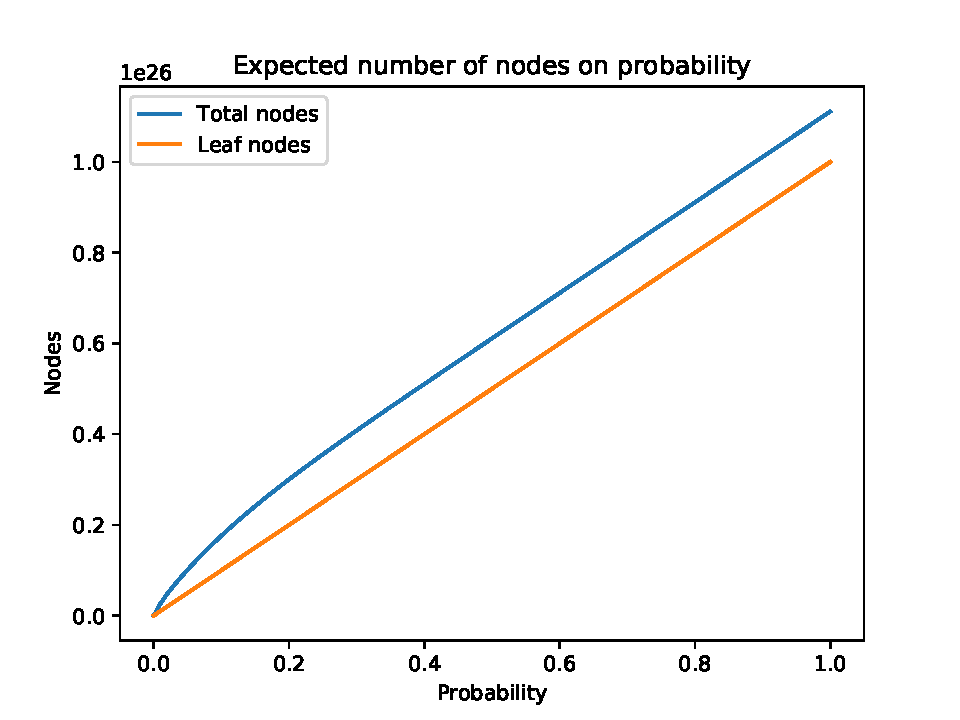
\includegraphics[width=.4\textwidth, keepaspectratio]{exp-nodes-on-probab.pdf}
\caption{$\mathbb{E}(|\mathcal{M}|)$ and $\mathbb{E}(|M|)$ on probability.}
\label{f:exp-nodes}
\end{figure}

As we see on the figure~\ref{f:exp-nodes} the value of $|\mathcal{M}|$ is slightly 
shifted with respect to the value of $|M|.$

Now we demonstrate a more descriptive comparison between $|\mathcal{M}|$ and 
$|M|.$ Figure~\ref{f:ratio-exp-msets} shows the ratio between the expected cardinality 
of a multiset-trie $|\mathcal{M}|$ and the actual number of multisets stored $|M|$ for 
parameters $n$ and $\sigma$ being $10$ and $26$ respectively.

\begin{figure}[h!]
\center
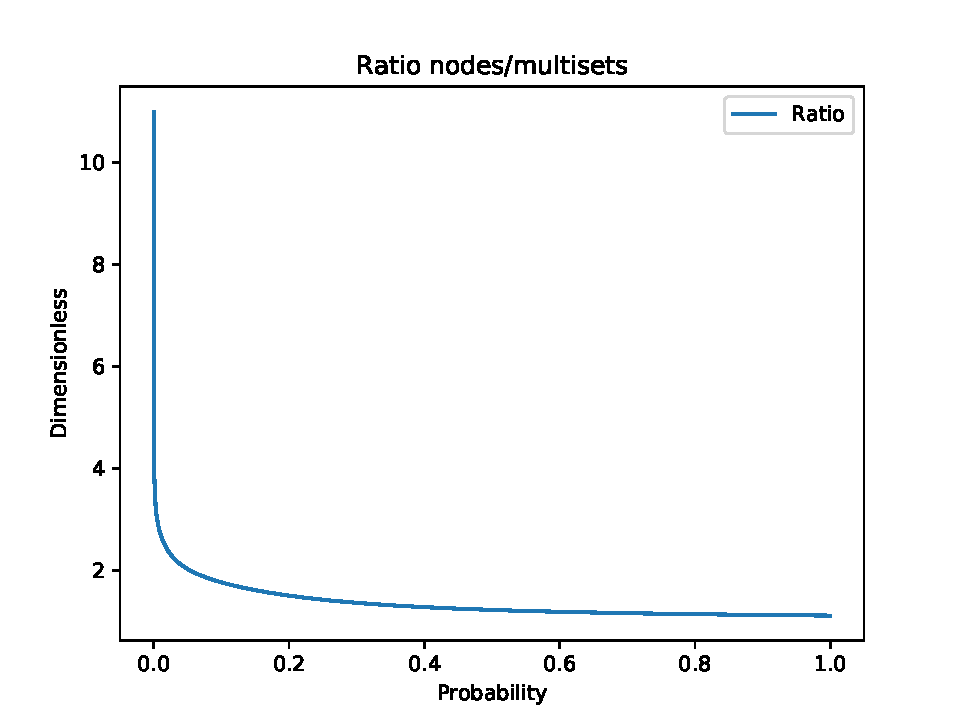
\includegraphics[width=.4\textwidth, keepaspectratio]{ratio-exp-nodes-and-msets-on-prob.pdf}
\caption{Ratio $\mathbb{E}(\frac{|\mathcal{M}|}{|M|})$ on $p.$}
\label{f:ratio-exp-msets}
\end{figure}

Note that analyzing the graph on figure~\ref{f:ratio-exp-msets} we can safely 
say that the upper bound for the ratio is $\sigma + 1.$ The argument holds, 
because of the limit 
\begin{equation}
\lim_{p\rightarrow 0^+} \mathbb{E}(\xi_i) = 1,
\end{equation}
where $\xi_i$ is the number of nodes on $i$-th level and $1\leq i \leq \sigma + 1.$ 

However, the ratio $\sigma + 1$ can be obtained only with a very small cardinality 
of the set $M,$ in particular $|M| = 1.$ In order to obtain such a case the 
probability $p$ must be at most $\frac{1}{n^\sigma}.$

The lower bound for the ratio is obviously at $p=1$ and is equal to 1
\begin{equation}
\lim_{n,\sigma \rightarrow\infty} \frac{n^{\sigma + 1} - 1}{n^\sigma (n-1)} = 1.
\end{equation}

Since the ratio $\sigma + 1$ can be obtained for a very specific case only and 
with a small increase \DIFdelbegin \DIFdel{of probability}\DIFdelend \DIFaddbegin \DIFadd{in probability, }\DIFaddend the ratio drops rapidly it can be concluded 
that the space complexity of the multiset-trie is $O(|M|).$






% section 5
\section{Experiments} \label{c:experiments}

%
This section contains \DIFaddbegin \DIFadd{the }\DIFaddend results of experiments that were performed on the multiset-trie 
data structure. In particular, we will test the functions: \textsc{submsetExistence}, 
\textsc{supermsetExistence}, \textsc{getAllSubmsets} and \textsc{getAllSupermsets}. 

The \DIFdelbegin \DIFdel{implementation of }\DIFdelend multiset-trie is \DIFdelbegin \DIFdel{done }\DIFdelend \DIFaddbegin \DIFadd{implemented }\DIFaddend in the \CC { programming} language. 
The current implementation uses only the standard library of \CC14 version of the 
standard and has a command line interface~\cite{akulich2019mstrie}. The implementation of the program was 
optimized for testing\DIFaddbegin \DIFadd{, }\DIFaddend and therefore, the program operates with files \DIFdelbegin \DIFdel{, in order }\DIFdelend to 
process queries. After processing all the queries\DIFaddbegin \DIFadd{, }\DIFaddend the results are stored in files for further analysis.

%Performance of the functions will be measured by 
%the number of visited nodes in multiset-trie by the particular function. In 
%particular the performance is inversely proportional to the number of visited 
%nodes.

Before we start, we will give a few definitions \DIFdelbegin \DIFdel{about }\DIFdelend \DIFaddbegin \DIFadd{of }\DIFaddend the parameters 
that will be varied throughout the experiments and discuss the experimental data 
that was used.

Let $M$ be a set of multisets \DIFdelbegin \DIFdel{that are }\DIFdelend inserted to multiset-trie and let $n$ be 
the maximal node degree. Let $N$ be the power multiset of $\Sigma,$ where 
the multiplicity of each element is bounded from above by $n-1.$ We define the 
\emph{density} of a multiset-trie to be the ratio $\frac{|M|}{|N|},$ where 
$|\cdot|$ denotes cardinality.

The selected parameters of the data structure that will be varied in \DIFaddbegin \DIFadd{the }\DIFaddend experiments 
are as follows:
%
\begin{itemize}
\item $\sigma$ - the cardinality of the alphabet $\Sigma;$
%
\item $n$ - the maximal degree of a node, which explicitly defines the maximal 
multiplicity of elements in a multiset;
%
\item $\phi$ - mapping of letters from $\Sigma$ into a set of consecutive 
integers;
%
\item $d$ - density of a multiset-trie.
%
\end{itemize}
The cardinality of a power multiset $N$ is equal to $n^\sigma,$ which means that 
density $d$ of a multiset-trie depends on parameters $|M|,$ $\sigma$ and $n.$ 
Because parameters $\sigma$ and $n$ are set when a multiset-trie is initialized, 
the parameter $|M|$ will be varied to change the density in experiments. As we 
mentioned in Section~\ref{c:description}, the mapping $\phi$ determines the 
correspondence of letters to levels in multiset-trie, i.e.\DIFaddbegin \DIFadd{, }\DIFaddend it defines the ordering of 
levels in multiset-trie. It is also true \DIFdelbegin \DIFdel{, }\DIFdelend that $\phi$ defines the ordering in multisets.

% anouncement of the experiments
In the \DIFdelbegin \DIFdel{next sections}\DIFdelend \DIFaddbegin \DIFadd{following sections, }\DIFaddend we will present the behavior of the multiset-trie data 
structure \DIFdelbegin \DIFdel{depending on the selected parameters as well as the comparative 
benchmark of the multiset-trie against B-tree implementation of inverted index.
%DIF <  outline of the experiment section
We start with experiments that are performed on an }\DIFdelend \DIFaddbegin \DIFadd{in four experiments.
The first three experiments use }\DIFaddend artificially generated data\DIFdelbegin \DIFdel{in 
order to give a general picture of the multiset-trie performance}\DIFdelend \DIFaddbegin \DIFadd{, and the fourth experiment
uses real-world data}\DIFaddend . In the 
Experiment~\hyperref[s:exp1]{1} a special case of the multiset-trie is considered. 
Only sets are allowed to be stored in the data structure, i.e.\DIFdelbegin \DIFdel{the maximal }\DIFdelend \DIFaddbegin \DIFadd{, the maximally }\DIFaddend allowed 
multiplicity is set to 1. The performance is measured with respect to the density 
of the multiset-trie.
%DIF < 
\DIFaddbegin 

\DIFaddend The Experiment~\hyperref[s:exp2]{2} is an extension of the previous one. Here, 
we also measure the performance of the multiset-trie depending on its density. 
The difference is that the allowed multiplicity of an element is raised, i.e. 
the data structure is populated with multisets. 
%DIF < 
\DIFaddbegin 

\DIFaddend Summarizing the tests of performance depending on the density\DIFaddbegin \DIFadd{, }\DIFaddend we present the 
Experiment~\hyperref[s:exp3]{3}. It shows a \DIFdelbegin \DIFdel{non linearity }\DIFdelend \DIFaddbegin \DIFadd{nonlinearity }\DIFaddend of the performance 
with respect to the density of the multiset-trie.
%DIF < 
\DIFdelbegin \DIFdel{The next }\DIFdelend \DIFaddbegin 

\DIFadd{Finally, the fourth }\DIFaddend experiment on the multiset-trie uses \DIFdelbegin \DIFdel{the real world }\DIFdelend \DIFaddbegin \DIFadd{real-world }\DIFaddend data. In 
Experiment~\hyperref[s:exp4]{4} the influence of the mapping $\phi$ is studied. 
The input data is obtained by mapping \DIFdelbegin \DIFdel{of }\DIFdelend the real words from \DIFaddbegin \DIFadd{the }\DIFaddend English dictionary 
to the set of consecutive integers using the function $\phi.$ The experiment 
shows that the performance of the multiset-trie is noticeably influenced by 
different mappings $\phi.$ It also shows the usability of the multiset-trie in terms 
of real data demonstrating the high performance of search queries.
\DIFaddbegin 

\DIFaddend % 
\DIFdelbegin \DIFdel{After all the experiments we present an empirical comparison of multiset-trie 
data structure with B-tree based inverted index. We use inverted index 
to store and retrieve multisets in the same way as it is described in the paper by 
Helmer and Moerkotte~\mbox{%DIFAUXCMD
\cite{Helmer2003} }\hspace{0pt}%DIFAUXCMD
for sets. In the comparison we use 
three types of queries exact, submultiset and supermultiset retrieval.
}\DIFdelend %DIF > After all the experiments we present an empirical comparison of multiset-trie 
%DIF > data structure with B-tree based inverted index. We use inverted index 
%DIF > to store and retrieve multisets in the same way as it is described in the paper by 
%DIF > Helmer and Moerkotte~\cite{Helmer2003} for sets. In the comparison we use 
%DIF > three types of queries exact, submultiset and supermultiset retrieval.

\subsection*{Data generation}
We denote by \emph{input data} the data that is used to fill the structure prior 
to testing and by \emph{test data} the set of queries that \DIFdelbegin \DIFdel{is }\DIFdelend \DIFaddbegin \DIFadd{are }\DIFaddend used to test the 
performance of the functions.

The artificially generated input data is obtained by sampling $|M|$ multisets 
from $N.$ All the multisets in $N$ are constructed according to parameters 
$\sigma$ and $n$ and represent the power multiset of the alphabet $\Sigma.$ 
Every multiset in $M$ is chosen from $N$ with equal probability $p.$ Thus, the 
probability $p$ gives a collection $M$ of multisets that are sampled from $N$ 
with uniform distribution. Uniform distribution is chosen in order to simulate
\DIFdelbegin \DIFdel{a 
}\DIFdelend random user input.

% test data explanation
The test data is generated artificially and constructed as follows. Given the 
parameters $\sigma$ and $n,$ the possible size of a multiset varies from~1 
to~$\sigma n.$ The number of randomly generated test multisets for every 
value of multiset size is 1500. In other words, we perform 1500 experiments 
in order to measure the number of visited nodes for the queries with \DIFaddbegin \DIFadd{a }\DIFaddend test multiset 
of \DIFdelbegin \DIFdel{a distinct size}\DIFdelend \DIFaddbegin \DIFadd{distinct sizes}\DIFaddend . The final value of visited nodes is calculated by taking an 
arithmetic mean among all 1500 measurements.


\subsection{Experiment 1} \label{s:exp1}
This experiment shows the performance of multiset-trie being used for storing 
and retrieving \emph{sets} instead of \emph{multisets}. We restrict multiset-trie in order 
to make a closer comparison with the \emph{set-trie} data structure~\cite{savnik2013index}.
In this case\DIFaddbegin \DIFadd{, }\DIFaddend we set the maximal node degree $n$ to be $2$ and $\sigma$ to be 25. 
The mapping $\phi$ does not have an influence in this particular experiment
\DIFdelbegin \DIFdel{, 
}\DIFdelend because the input data is generated artificially with uniform distribution. On 
average\DIFaddbegin \DIFadd{, }\DIFaddend the results will be the same for any $\phi,$ since all the multisets are 
equally likely to appear in $M.$ The parameter $|M|$ varies from 10000 sets up 
to 320000 sets. According to the parameters $n$ and $\sigma,$ the cardinality of 
$N$ is $33554432\approx \num{3.36e+7}.$ Thus, the calculated density of the 
multiset-trie with respect to $|M|$ varies from~$\num{0.3e-3}$ to~$\num{9.5e-3}.$


\begin{figure}
	\center
	\subcaptionbox{submsetExistence \label{fig:e1m1}}{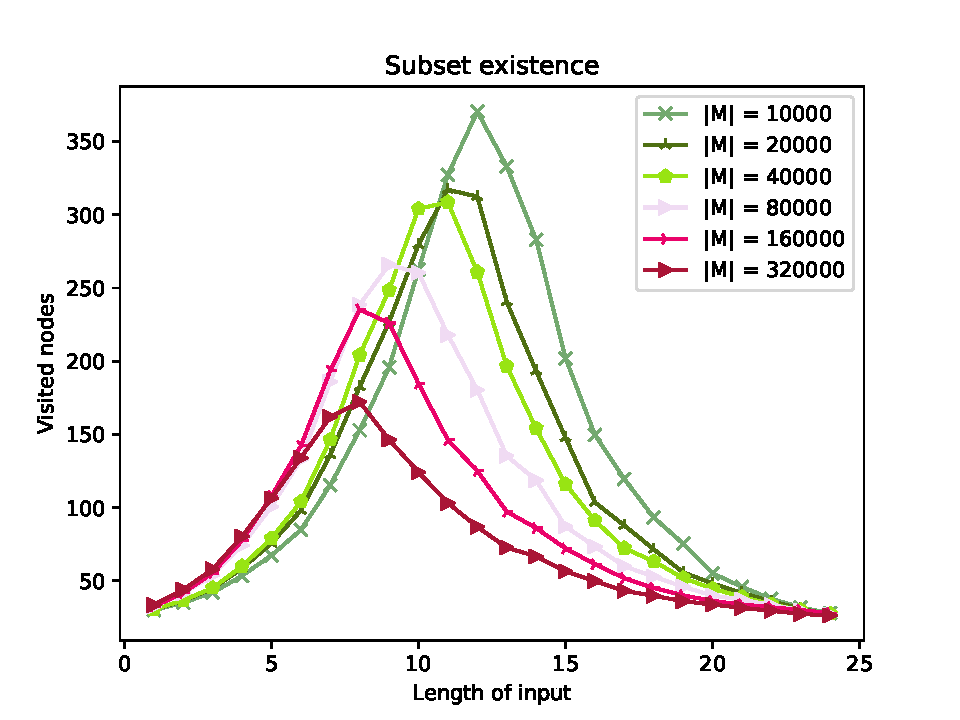
\includegraphics[width=.45\textwidth]{exp1-m1.pdf}}
	\subcaptionbox{supermsetExistence\label{fig:e1m2}}{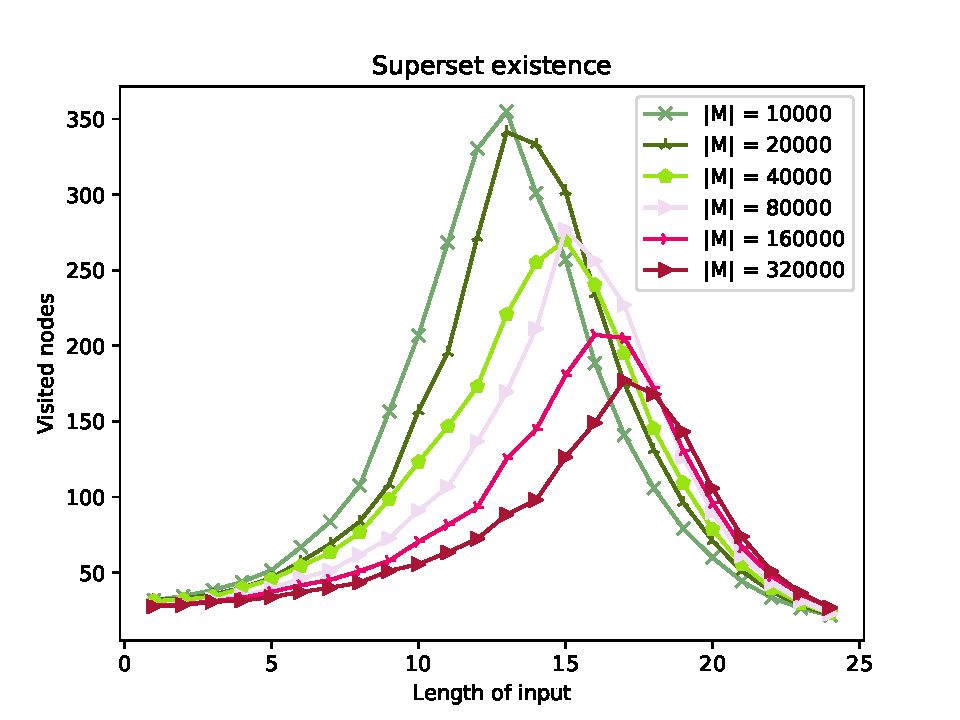
\includegraphics[width=.45\textwidth]{exp1-m2.pdf}}
	\caption{Existence functions of Experiment 1.}
\end{figure}

\begin{figure}[ht]
\center
\subcaptionbox{getAllSubmsets
\label{fig:e1m3}}{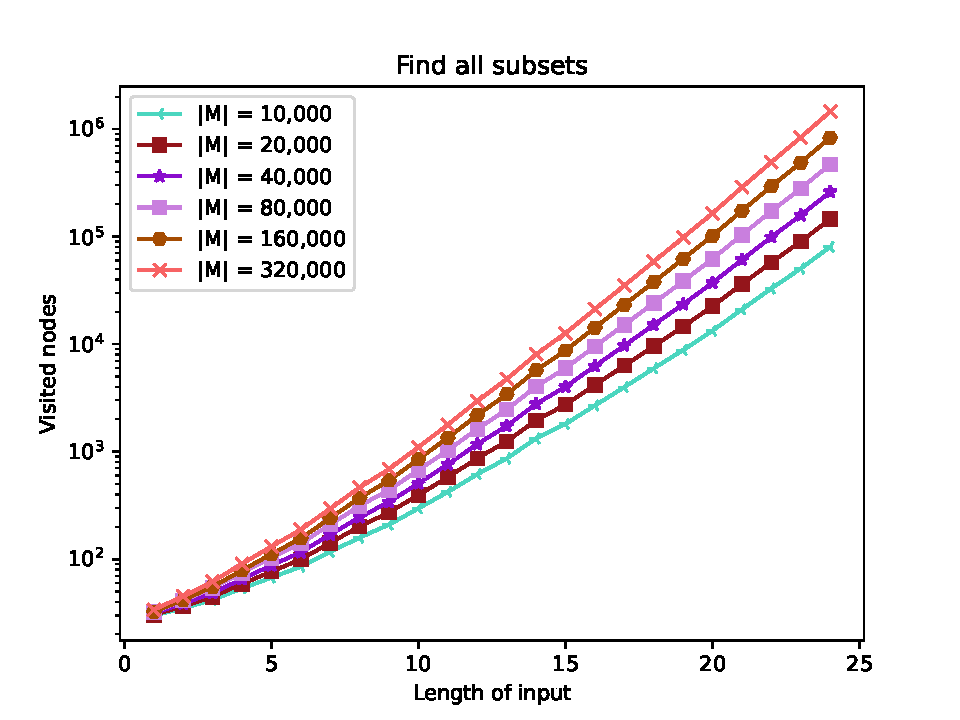
\includegraphics[width=.45\textwidth]{exp1-m3.pdf}
}
\subcaptionbox{getAllSupermsets
\label{fig:e1m4}}{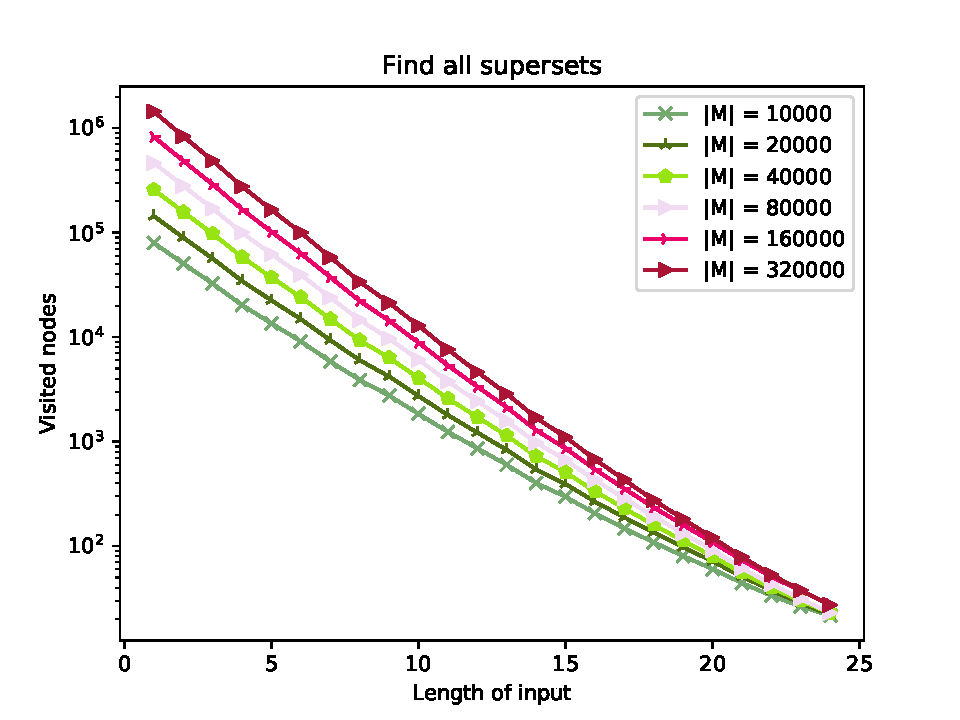
\includegraphics[width=.45\textwidth]{exp1-m4.pdf}
}
\caption{Exhaustive functions of Experiment 1.}
\end{figure}

The performance of the functions \textsc{submsetExistence} and 
\textsc{supermsetExistence} increases as the density increases (see figures~\ref{fig:e1m1}
and~\ref{fig:e1m2}). The results are as expected \DIFdelbegin \DIFdel{, }\DIFdelend because the increase of the 
density increases the probability of finding \DIFdelbegin \DIFdel{submultiset or supermultiset }\DIFdelend \DIFaddbegin \DIFadd{sub-multiset or super-multiset }\DIFaddend in 
multiset-trie, which leads to \DIFdelbegin \DIFdel{the }\DIFdelend \DIFaddbegin \DIFadd{a }\DIFaddend lower number of visited nodes. 

The maxima are located between 175 and 375 for \textsc{submsetExistence} and 
between 175 and 350 for \textsc{supermsetExistence}. According to those maxima 
we can deduce that at least 7-15 multisets were checked in order to find 
\DIFdelbegin \DIFdel{submultiset or supermultiset}\DIFdelend \DIFaddbegin \DIFadd{sub-multiset or super-multiset}\DIFaddend , which is from $\num{0.02e-3}$ to $\num{1.5e-3}$ of the 
multiset-trie and from $\num{1.9e-7}$ to $\num{4.5e-7}$ of the complete 
multiset-trie.

As the density increases\DIFaddbegin \DIFadd{, }\DIFaddend the peaks shift from the center to the left \DIFdelbegin \DIFdel{, }\DIFdelend or to the right, 
for \textsc{submsetExistence} and \textsc{supermsetExistence} respectively. 
The shifts are the consequence of the uniform distribution of sets in $M.$ 
Since every set has the same probability \DIFdelbegin \DIFdel{to appear }\DIFdelend \DIFaddbegin \DIFadd{of appearing }\DIFaddend in $M,$ the distribution of set 
sizes in $M$ is normal. Consequently, with \DIFdelbegin \DIFdel{increase of }\DIFdelend \DIFaddbegin \DIFadd{the increase in }\DIFaddend the density of the 
multiset-trie the number of sets in $M$ with cardinality $\frac{1}{2}\sigma$ will be 
larger than the number of sets with cardinality $\frac{1}{2}\sigma\pm\epsilon,$ 
for $\frac{1}{2}\sigma > \epsilon > 0.$ So the function \textsc{submsetExistence} 
needs to visit less nodes for test sets of size $\frac{1}{2}\sigma$ than for test 
sets of size $\frac{1}{2}\sigma\pm\epsilon.$ The function decreases the 
multiplicity of some elements (in some cases skips them) in order to find the 
closest subset. Hence, the peak shifts to the left. Oppositely the function 
\textsc{supermsetExistence} increases the multiplicity of some elements 
(in this case\DIFaddbegin \DIFadd{, }\DIFaddend adding new elements) in order to find the closest superset. 
Thus, the peak shifts to the right.

Note that despite the peak shifts both functions \textsc{submsetExistence} and 
\textsc{supermsetExistence} have approximately the same \DIFdelbegin \DIFdel{worst case }\DIFdelend \DIFaddbegin \DIFadd{worst-case }\DIFaddend performance. 

The performance of the functions \textsc{getAllSubmsets} and \textsc{getAllSupermsets} 
decreases as the density increases (see figures~\ref{fig:e1m3} and~\ref{fig:e1m4}). 
This happens because the number of multisets in multiset-trie increases, which means 
that any multiset in the data structure will have more sub- and \DIFdelbegin \DIFdel{supermultisets}\DIFdelend \DIFaddbegin \DIFadd{super-multisets}\DIFaddend . 
The maxima for both functions varies from $\num{8.0e4}$ to $\num{1.5e6}$ visited nodes. 
We can notice that local maxima for the functions \textsc{getAllSubmsets} and 
\textsc{getAllSupermsets} differs with respect to the length of input. The 
explanation is very simple. In order to find all submultisets of a small set the 
function has to traverse a small part of \DIFdelbegin \DIFdel{multist-trie}\DIFdelend \DIFaddbegin \DIFadd{the multiset-trie}\DIFaddend . As the size of a set 
increases\DIFaddbegin \DIFadd{, }\DIFaddend the part of a multiset-trie where all the submultisets of a given set 
are stored also increases. The opposite holds for the function 
\textsc{getAllSupermsets}.


Despite the fact that for a lookup of any set/multiset $\sigma$ nodes must be visited 
in multiset-trie on average case, the data structure has a very similar performance 
results in comparison to the \emph{set-trie} data structure.

\subsection{Experiment 2} \label{s:exp2}
In the Experiment~\hyperref[s:exp2]{2} we demonstrate the performance of 
the unrestricted multiset-trie allowing \emph{multisets} to be inserted into \DIFaddbegin \DIFadd{the }\DIFaddend data structure. 
We set $n$ to be 6 and retain $\sigma = 25$ as it was in Experiment~\hyperref[s:exp1]{1}. 
The mapping $\phi$ does not have an influence on \DIFaddbegin \DIFadd{the }\DIFaddend results, since the input 
data is generated artificially with uniform distribution. The cardinality of $M$ 
varies from 40000 to 640000 multisets. Thus, the calculated density $d$ varies 
from $\num{1.4e-15}$ to $\num{2.25e-14}.$ The density is much smaller than 
in Experiment~\hyperref[s:exp1]{1}, because now we allow multisets to be stored 
in the data structure and according to the parameters $n$ and $\sigma$ the 
cardinality of $N$ is $6^{25} = \num{2.84e19}.$

\begin{figure}[ht]
\center

\subcaptionbox{submsetExistence
\label{fig:e2m1}}{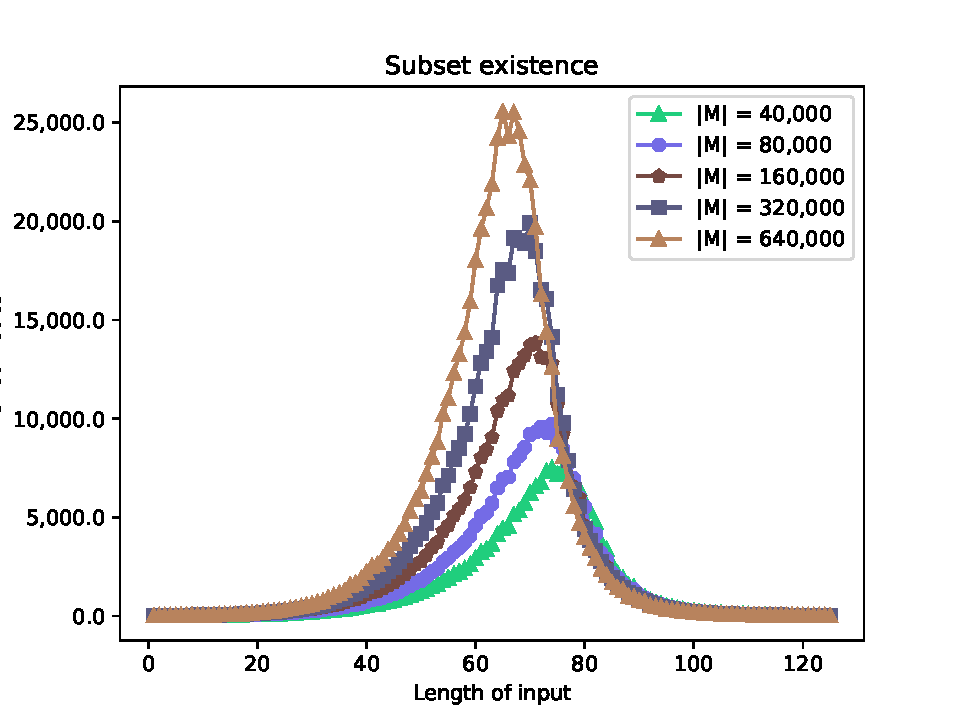
\includegraphics[width=.45\textwidth]{exp2-m1.pdf}}
\subcaptionbox{supermsetExistence
\label{fig:e2m2}}{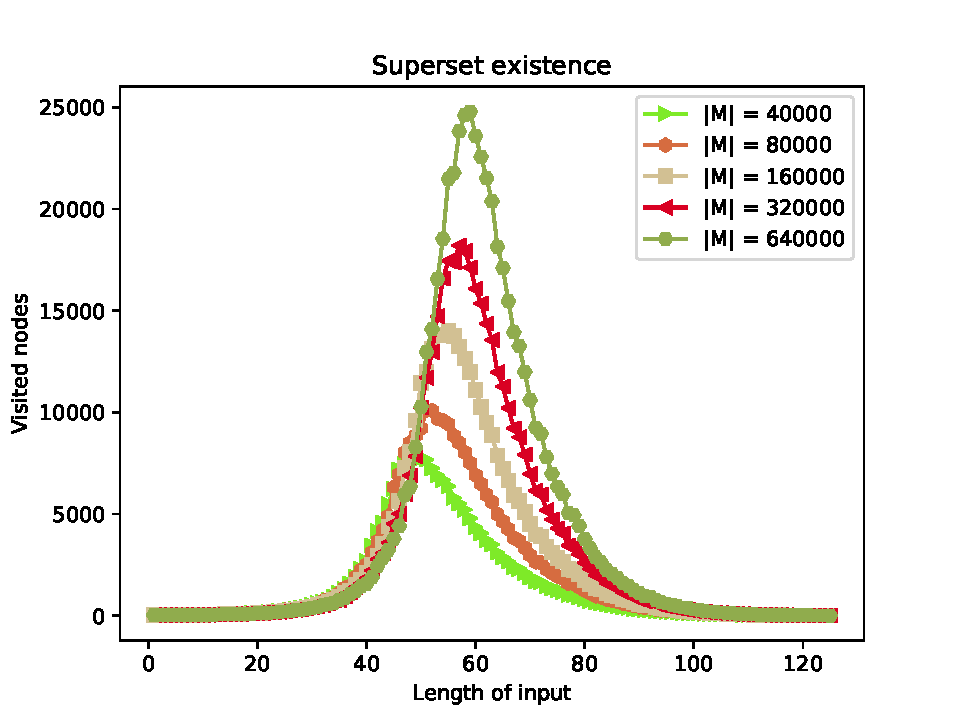
\includegraphics[width=.45\textwidth]{exp2-m2.pdf}}
\caption{Existence functions in Experiment 2.}
\end{figure}

\begin{figure}[ht]
\center
\subcaptionbox{Experiment 2, getAllSubmsets function.
\label{fig:e2m3}}{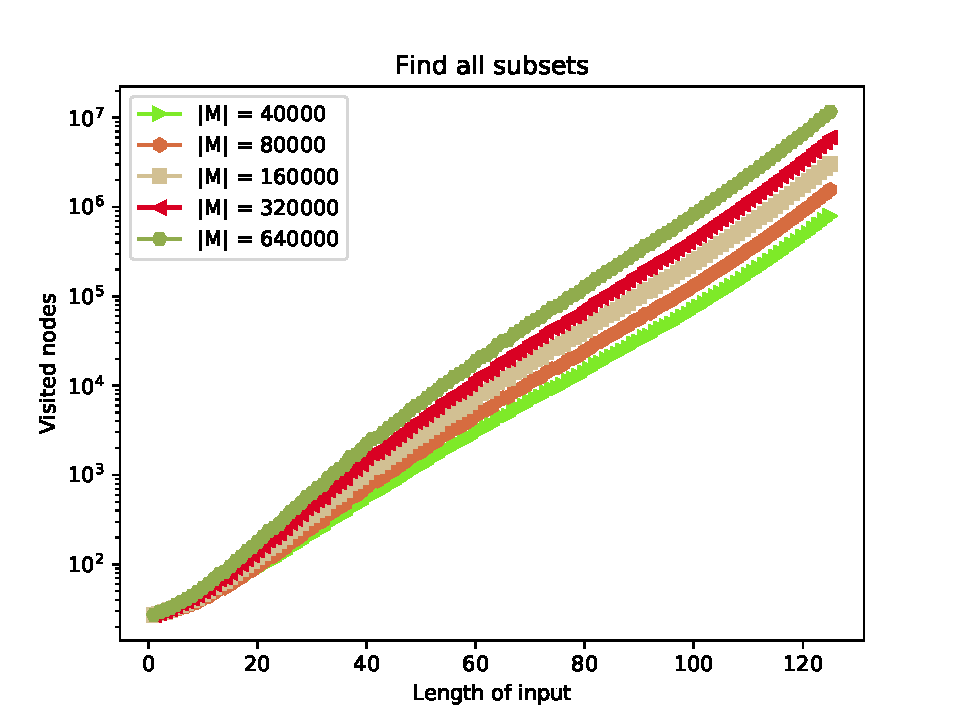
\includegraphics[width=.45\textwidth]{exp2-m3.pdf}}
\subcaptionbox{Experiment 2, getAllSupermsets function.
\label{fig:e2m4}}{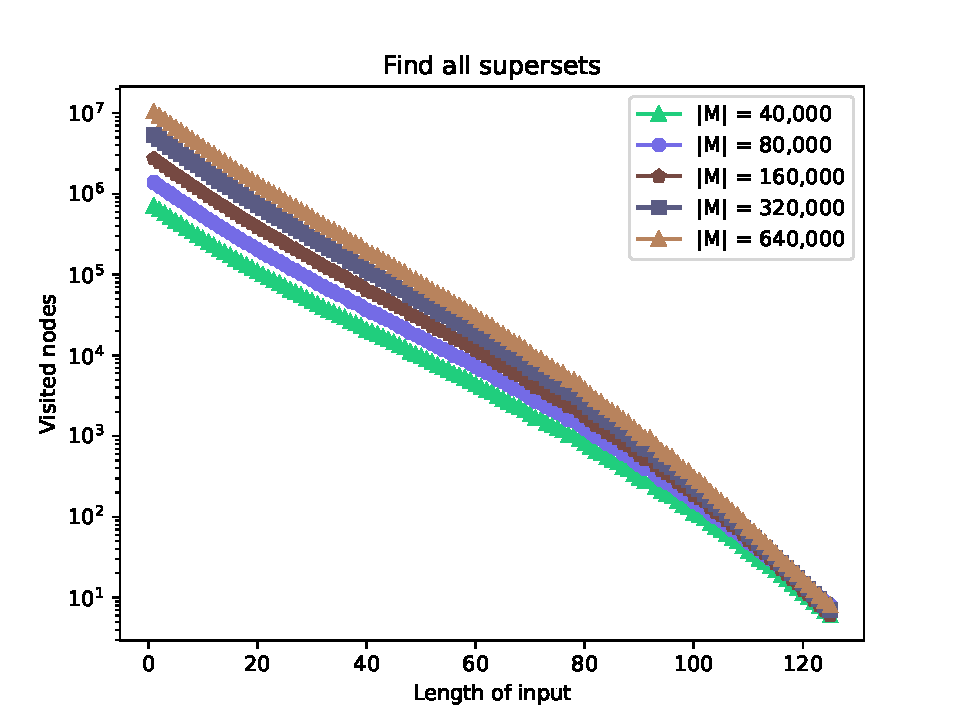
\includegraphics[width=.45\textwidth]{exp2-m4.pdf}}
\caption{Exhaustive functions in Experiment 2.}
\end{figure}

As we can see from the graphs on figures~\ref{fig:e2m1} and~\ref{fig:e2m2}, 
the performance of the functions \textsc{submsetExistence} and 
\textsc{supermsetExistence} becomes worse as the density increases. 
In this case\DIFaddbegin \DIFadd{, }\DIFaddend the number $|M|$ is slightly larger than in the 
Experiment~\hyperref[s:exp1]{1}, but the density is very small. Consequently\DIFaddbegin \DIFadd{, 
}\DIFaddend multiset-trie \DIFdelbegin \DIFdel{become }\DIFdelend \DIFaddbegin \DIFadd{becomes }\DIFaddend more sparse. Multisets in a sparse multiset-trie \DIFdelbegin \DIFdel{differs }\DIFdelend \DIFaddbegin \DIFadd{differ }\DIFaddend more, 
which leads to \DIFdelbegin \DIFdel{the }\DIFdelend \DIFaddbegin \DIFadd{a }\DIFaddend larger number of visited nodes. 

The maxima for both functions \DIFdelbegin \DIFdel{varies }\DIFdelend \DIFaddbegin \DIFadd{vary }\DIFaddend from 7500 to 25000 visited nodes. According 
to those maxima\DIFaddbegin \DIFadd{, }\DIFaddend at least 300-1000 multisets were checked in order to find 
\DIFdelbegin \DIFdel{submultiset or supermultiset}\DIFdelend \DIFaddbegin \DIFadd{sub-multiset or super-multiset}\DIFaddend , which is from $\num{1.5e-3}$ to $\num{7.5e-3}$ of the entire 
multiset-trie and from $\num{1.1e-17}$ to $\num{3.4e-17}$ of the complete 
multiset-trie. The percentage of visited multisets with respect to $|M|$ is 
larger than in the Experiment~\hyperref[s:exp1]{1}. However, if one would compare 
the percentage of visited multiset with respect to complete multiset-trie, then 
in \DIFaddbegin \DIFadd{the }\DIFaddend case of Experiment~\hyperref[s:exp2]{2} it is less by 10 orders than in the 
Experiment~\hyperref[s:exp1]{1}.

The peaks are shifted from the center to the left and right for 
\textsc{submsetExistence} and \textsc{supermsetExistence} respectively. Such 
\DIFdelbegin \DIFdel{a 
}\DIFdelend behavior was previously observed in the Experiment~\hyperref[s:exp1]{1}. The 
explanation is the same: the input data has \DIFaddbegin \DIFadd{a }\DIFaddend uniform distribution, implying that 
the size of multisets in $M$ is normally distributed. Because of the normal 
distribution of \DIFaddbegin \DIFadd{the }\DIFaddend size of multisets\DIFaddbegin \DIFadd{, }\DIFaddend the shift of the peak occurs as the density increases.

It can \DIFdelbegin \DIFdel{be also observed that }\DIFdelend \DIFaddbegin \DIFadd{also be observed that, }\DIFaddend as in previous Experiment~\hyperref[s:exp1]{1}\DIFaddbegin \DIFadd{, }\DIFaddend both 
functions \textsc{submsetExistence} and \textsc{supermsetExistence} have similar 
\DIFdelbegin \DIFdel{worst case }\DIFdelend \DIFaddbegin \DIFadd{worst-case }\DIFaddend performance. 

The functions \textsc{getAllSubmsets} and \textsc{getAllSupermsets} decrease 
their performance as the density increases (see figures~\ref{fig:e2m3} 
and~\ref{fig:e2m4}). \DIFdelbegin \DIFdel{It happens , }\DIFdelend \DIFaddbegin \DIFadd{This happens }\DIFaddend because the number of multisets increases as 
the density increases. So there are more nodes \DIFaddbegin \DIFadd{that }\DIFaddend have to be visited in order to 
retrieve all sub- or \DIFdelbegin \DIFdel{supermultisets }\DIFdelend \DIFaddbegin \DIFadd{super-multisets }\DIFaddend of some multiset. The maximum for both functions 
varies from $\num{0.9e5}$ to $\num{1.5e7}$ visited nodes. As it was observed in 
Experiment~\hyperref[s:exp1]{1}\DIFaddbegin \DIFadd{, }\DIFaddend the maxima occur at the opposite points. For the 
function \textsc{getAllSubmsets} it will always be at the largest size of \DIFaddbegin \DIFadd{the }\DIFaddend multiset, 
which is 125 in our case. Conversely the maximum for the \textsc{getAllSupermsets} 
is at the smallest size of multiset, which is 0 (an empty set).

The results of the Experiment~\hyperref[s:exp1]{1} show that the performance 
of functions \textsc{submsetExistence} and \textsc{supermsetExistence} increases 
as the density increases. However, we observe the opposite behavior in the 
Experiment~\hyperref[s:exp2]{2}. We explain the reason of such a contradiction 
in the next Experiment~\hyperref[s:exp3]{3} 


%DIF < \subsection{Experiment 3}
%DIF < In this experiment we vary $\sigma$ from 10 up to 70. The maximal degree node 
%DIF < $n$ is set to 6 and the input data $|M|$ is set to 640000 multisets. This way 
%DIF < we extremly decrease density $d$ as we increase $\sigma.$ 
%DIF < The density varies from $1.0\%$ to $\num{2.1e-47}\%.$
%DIF < 
%DIF < \begin{figure}
%DIF < \center
%DIF < 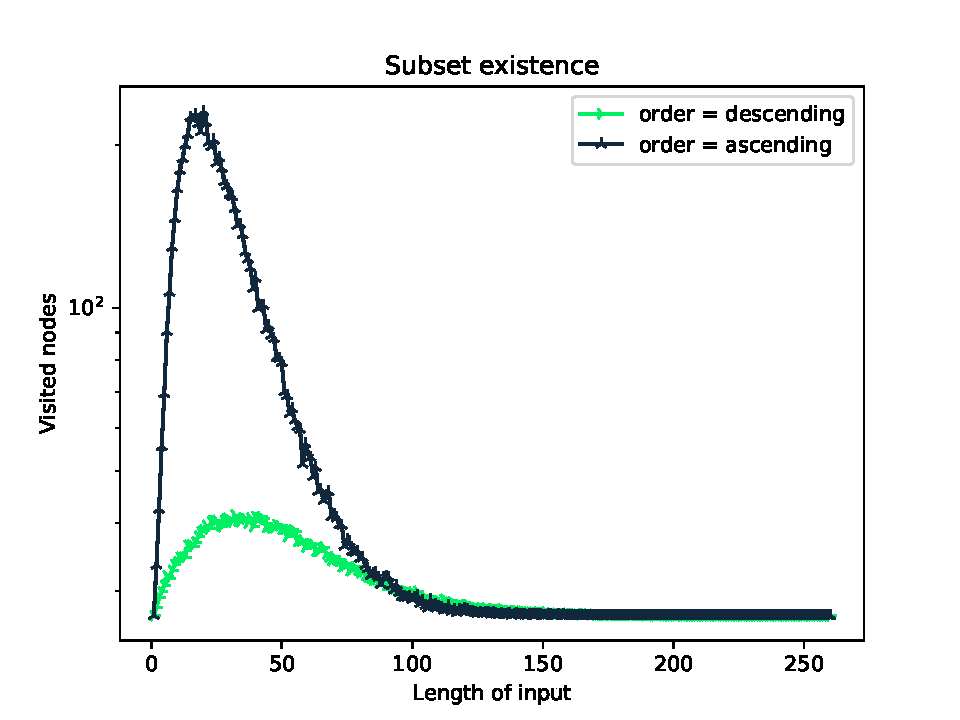
\includegraphics[width=.9\textwidth]{exp3-m1.pdf}
%DIF < \caption{Experiment 3, submsetExistence function.}
%DIF < \end{figure}
%DIF < 
%DIF < \begin{figure}
%DIF < \center
%DIF < 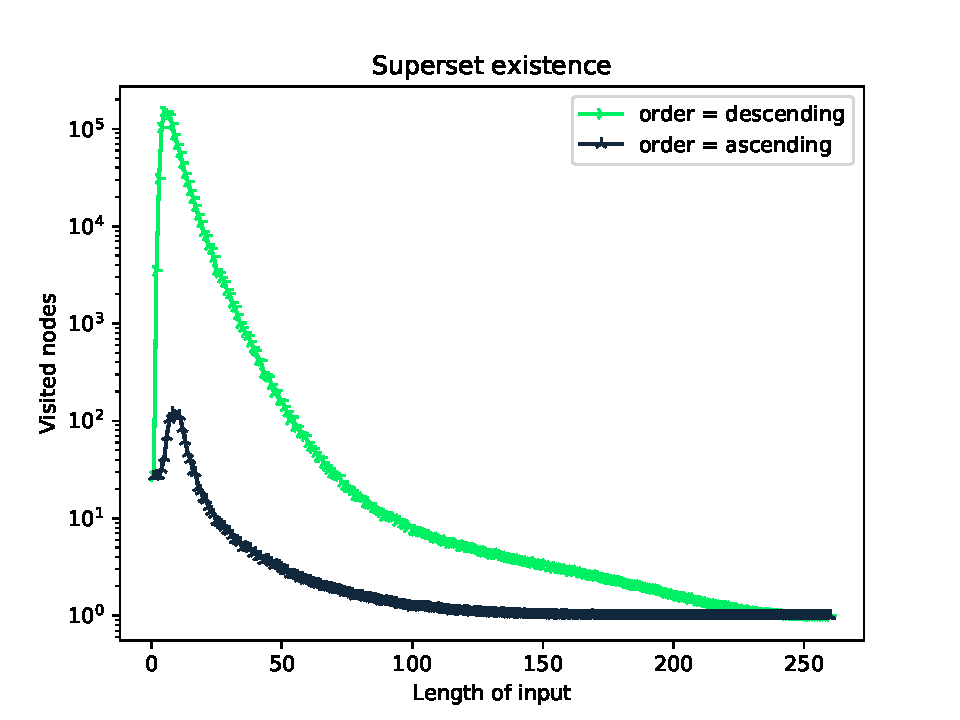
\includegraphics[width=.9\textwidth]{exp3-m2.pdf}
%DIF < \caption{Experiment 3, supermsetExistence function.}
%DIF < \end{figure}
%DIF < 
%DIF < \begin{figure}
%DIF < \center
%DIF < \includegraphics[width=.9\textwidth]{exp3-m3.pdf}
%DIF < \caption{Experiment 3, getAllSubmsets function.}
%DIF < \end{figure}
%DIF < 
%DIF < \begin{figure}
%DIF < \center
%DIF < \includegraphics[width=.9\textwidth]{exp3-m4.pdf}
%DIF < \caption{Experiment 3, getAllSupermsets function.}
%DIF < \end{figure}
\DIFdelbegin %DIFDELCMD < 

%DIFDELCMD < %%%
\DIFdelend \subsection{Experiment 3} \label{s:exp3}
The results of the Experiment~\hyperref[s:exp1]{1} and Experiment~\hyperref[s:exp2]{2} 
have shown that as the density of a multiset-trie increases the performance of 
functions \textsc{submsetExistence} and \textsc{supermsetExistence} can both get 
better and worse. The reason \DIFdelbegin \DIFdel{of }\DIFdelend \DIFaddbegin \DIFadd{for }\DIFaddend such a behavior is that the dependence of the 
number of visited nodes on density is not a linear function. 
\DIFdelbegin \DIFdel{It is obvious that the 
}\DIFdelend \DIFaddbegin \DIFadd{The }\DIFaddend performance of the \DIFdelbegin \DIFdel{mentioned above }\DIFdelend \DIFaddbegin \DIFadd{abovementioned }\DIFaddend functions is maximal when multiset-trie is 
complete. As multiset-trie becomes more sparse (the density is small)\DIFaddbegin \DIFadd{, }\DIFaddend multisets
differ more\DIFaddbegin \DIFadd{, }\DIFaddend and the number of visited nodes increases. However, \DIFaddbegin \DIFadd{multisets differ
less }\DIFaddend when the density is high, \DIFdelbegin \DIFdel{multisets differ less, }\DIFdelend so the number of visited nodes decreases. Since 
the dependence of the number of visited nodes on the density of multiset-trie 
is a continuous function on the interval $[0,1],$ there exists a global maximum. 
In other words\DIFaddbegin \DIFadd{, }\DIFaddend there exists such a value of density where the number of visited 
nodes is maximal. 

In this experiment, we empirically find the extremum of density for functions 
\textsc{submsetExistence} and \textsc{supermsetExistence}. The parameters 
$\sigma$ and $n$ are set to 12 and 5\DIFaddbegin \DIFadd{, }\DIFaddend respectively. The density varies from 
$\num{1.0e-6}$ to $\num{1.0e-2}.$ The number of visited nodes was chosen to be 
maximal for each value of \DIFaddbegin \DIFadd{a }\DIFaddend particular density.

\begin{figure}
\center
\subcaptionbox{submsetExistence
\label{fig:e3m1}}{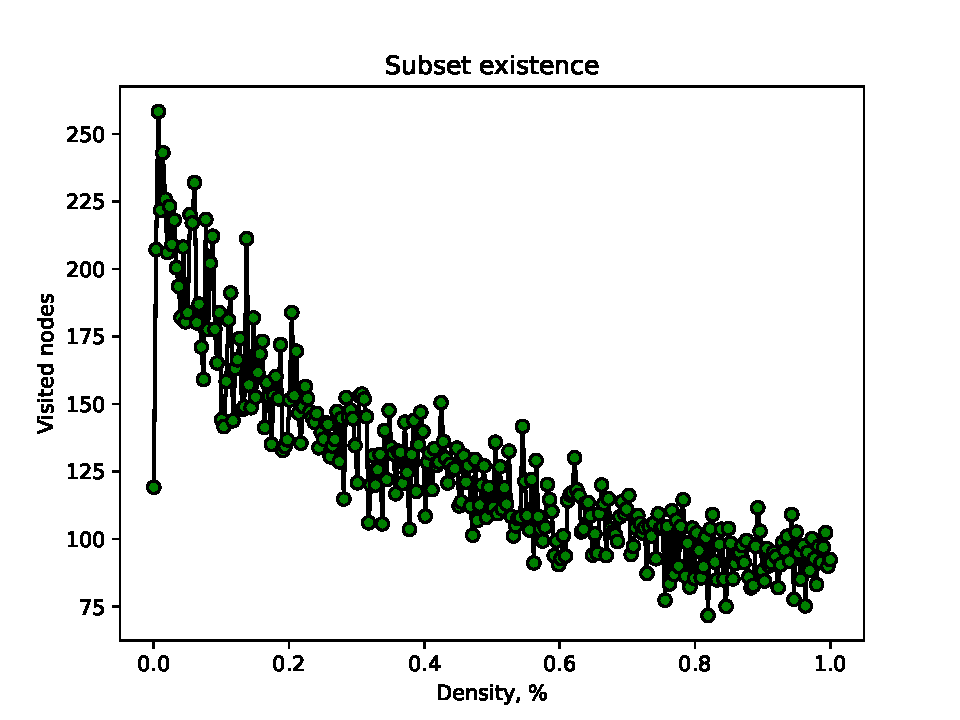
\includegraphics[width=.45\textwidth]{exp4-m1.pdf}}
\subcaptionbox{supermsetExistence
\label{fig:e3m2}}{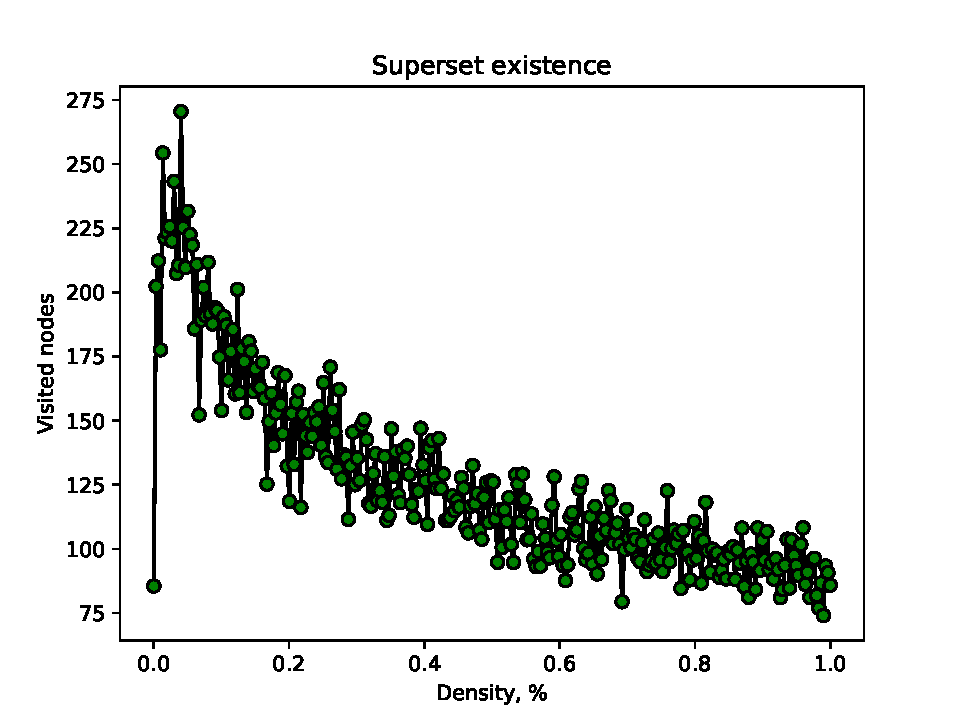
\includegraphics[width=.45\textwidth]{exp4-m2.pdf}}
\caption{Exsitence functions in Experiment 3.}
\end{figure}

As we see on figures~\ref{fig:e3m1} and~\ref{fig:e3m2} both functions 
\textsc{submsetExistence} and \textsc{supermsetExistence} have the maximum 
around $d\approx \num{7.0e-5}.$ The maximum is less than $\num{0.3e-3}$ and 
greater than $\num{1.4e-15},$ which explains the behavior of multiset-trie in 
Experiment~\hyperref[s:exp1]{1} and Experiment~\hyperref[s:exp2]{2}. It is safe 
to say that the maximum may vary depending on parameters $n$ and $\sigma,$ but 
such a maximum always exists. Therefore, we omit the experiments with different 
parameters $n$ and $\sigma.$


\subsection{Experiment 4} \label{s:exp4}
In previous experiments\DIFaddbegin \DIFadd{, }\DIFaddend the input was generated artificially with uniform 
distribution, so there was no influence of the mapping function $\phi$ on 
\DIFaddbegin \DIFadd{the }\DIFaddend performance of tested functions. This experiment shows the influence of the 
mapping $\phi$ from alphabet $\Sigma$ to a set of consecutive integers. 
We obtain the influence by taking the \DIFdelbegin \DIFdel{real world data as an }\DIFdelend \DIFaddbegin \DIFadd{real-world data as }\DIFaddend input data. 

The data is taken from \DIFdelbegin \DIFdel{English dictionary }\DIFdelend \DIFaddbegin \DIFadd{the English dictionary, }\DIFaddend which contains 235883 different words. 
Those words are mapped to multisets of integers according to the $\phi.$ In 
particular, we are interested in cases when $\phi(\Sigma)$ enumerates 
letters by their relative frequency in \DIFaddbegin \DIFadd{the }\DIFaddend English language. We say that $\phi(\Sigma)$ 
maps letters in \emph{ascending order} if the most frequent letter is mapped to 
number $\sigma.$ Conversely, in \emph{descending order} this letter is mapped to 
\DIFaddbegin \DIFadd{the }\DIFaddend number $1.$ The size of the alphabet $\sigma$ is set to the size of the English 
alphabet 26. The degree of a node $n$ is set to 10. On average\DIFaddbegin \DIFadd{, }\DIFaddend the multiplicity 
of letters is\DIFdelbegin \DIFdel{of course }\DIFdelend \DIFaddbegin \DIFadd{, of course, }\DIFaddend less than 10. We choose such a large node degree allowing 
the multiplicity to be up to 10 \DIFdelbegin \DIFdel{, }\DIFdelend because the dictionary contains such words. 


\begin{figure}
\center
\subcaptionbox{submsetExistence
\label{fig:e4m1}}{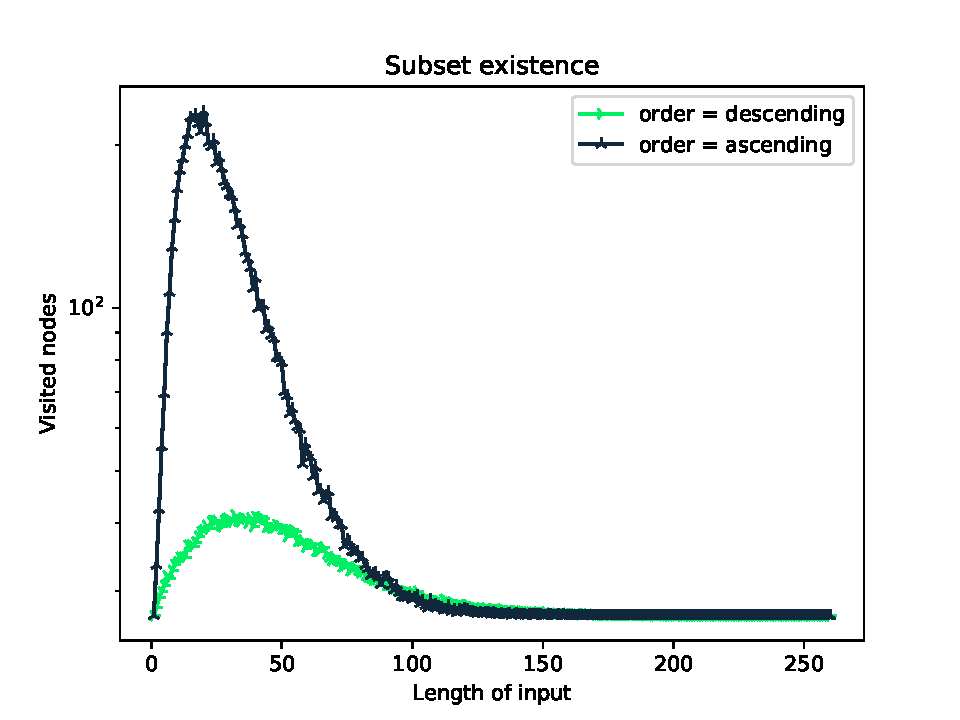
\includegraphics[width=.45\textwidth]{exp3-m1.pdf}}
\subcaptionbox{supermsetExistence
\label{fig:e4m2}}{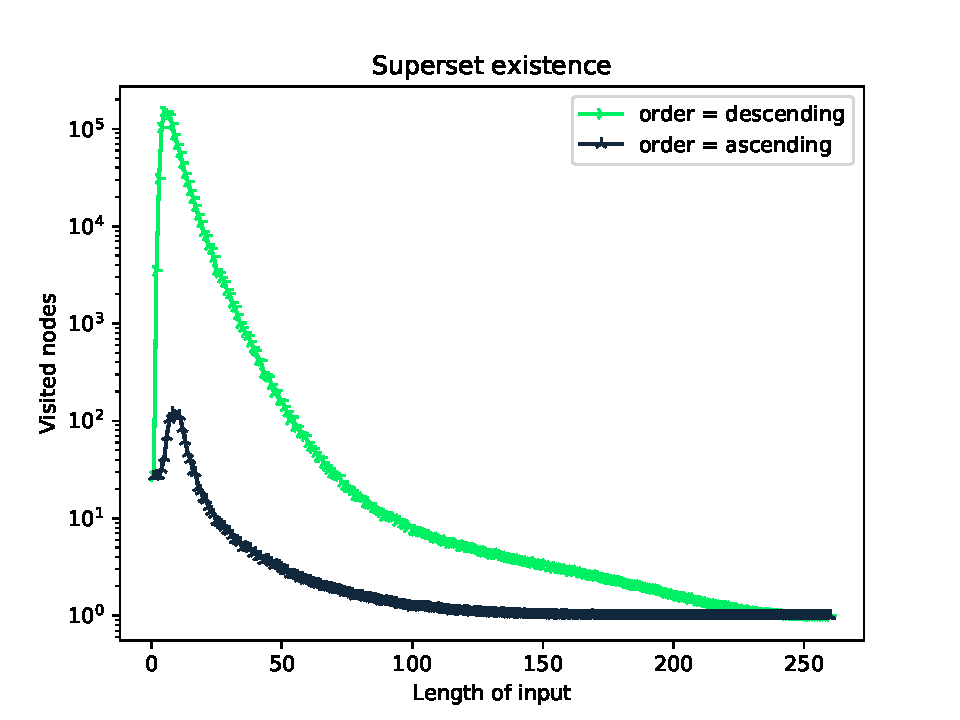
\includegraphics[width=.45\textwidth]{exp3-m2.pdf}}
\caption{Existence functions in Experiment 4.}
\end{figure}

%\begin{figure}
%\includegraphics[width=\textwidth]{exp4-m3.pdf}
%\caption{Experiment 4, getAllSubmsets function.}
%\end{figure}
%
%\begin{figure}
%\includegraphics[width=\textwidth]{exp4-m4.pdf}
%\caption{Experiment 4, getAllSupermsets function.}
%\end{figure}

The results on figures~\ref{fig:e4m1} and~\ref{fig:e4m2} are more balanced when 
letters are ordered by frequency in ascending order. The maxima for the functions 
\textsc{submsetExistence} and \textsc{supermsetExistence} are at 250 visited nodes. 

According to the design of the data structure multiset-trie, we can say 
something about multiset only if we try to reach it, i.e.\DIFaddbegin \DIFadd{, }\DIFaddend to find the complete 
path that corresponds to a particular multiset. \DIFdelbegin \DIFdel{It }\DIFdelend \DIFaddbegin \DIFadd{This }\DIFaddend means that in order to give 
an answer \DIFdelbegin \DIFdel{whether some multisetexists or not one have }\DIFdelend \DIFaddbegin \DIFadd{about the existance of some multiset, one has }\DIFaddend to check the leaf level in 
multiset-trie. 

Letters that have the least frequencies are now located at the top of 
multiset-trie according to ascending order of letters by frequency. This means 
that the search becomes narrower \DIFdelbegin \DIFdel{, }\DIFdelend because a lot of invalid paths will be 
discarded on top most levels. Thus, multiset-trie can be traversed faster.

As you may have noticed the functions \textsc{getAllSubmsets} and 
\textsc{getAllSupermsets} were not tested in this experiment. Those functions 
are not affected by variations of the mapping $\phi,$ because for any multiset\DIFaddbegin \DIFadd{, 
}\DIFaddend they retrieve all sub/supermultisets. This means that the number of visited 
nodes will not be changed as $\phi$ varies.
\DIFdelbegin %DIFDELCMD < 

%DIFDELCMD < %%%
\subsection{\DIFdel{Experiment 5}} %DIFAUXCMD
\addtocounter{subsection}{-1}%DIFAUXCMD
%DIFDELCMD < \label{s:exp5}
%DIFDELCMD < %%%
\DIFdel{In this experiment, we demonstrate the performance of multiset-trie data structure compared to the inverted index based on the B-tree. Both data structures are implemented in the programming language }%DIFDELCMD < \CC%%%
\DIFdel{, providing in this way an experimental setup for a fair comparison \mbox{%DIFAUXCMD
\cite{akulich2019mstrie}}\hspace{0pt}%DIFAUXCMD
.
}%DIFDELCMD < 

%DIFDELCMD < %%%
%DIF < ((Brief description of the implementation of the inverted files?))
\DIFdel{The inverted index is implemented using an idea from~\mbox{%DIFAUXCMD
\cite{Helmer2003}}\hspace{0pt}%DIFAUXCMD
. An inverted index structure consist of two parts: a dictionary and postings. In our case a dictionary is implemented as an in-memory B-tree where keys are all distinct values from a domain represented by a set $\Sigma.$ The postings are represented by lists of multisets that contain a particular element from $\Sigma.$ Each list item in postings contains a cardinality of a multiset, which speeds up the containment queries.
}%DIFDELCMD < 

%DIFDELCMD < %%%
\DIFdel{The experiment uses the input data for the construction of the given data structure and the test data for the execution of the operations on the given data structure. The input data comprises a set of randomly generated multisets used for the construction of a data structure. The test data includes the set of multisets together with the operations that are evaluated. The input and test data were generated with respect to parameters $\sigma$ and $n$ as presented in Table~\ref{t:benchmark}.
}%DIFDELCMD < 

%DIFDELCMD < \begin{table}[h]
%DIFDELCMD < \center
%DIFDELCMD < \begin{tabular}{|c|c|}
%DIFDELCMD < \hline
%DIFDELCMD < %%%
\DIFdelFL{$\sigma$ }%DIFDELCMD < & %%%
\DIFdelFL{$n$ }%DIFDELCMD < \\
%DIFDELCMD < \hline
%DIFDELCMD < %%%
\DIFdelFL{5		}%DIFDELCMD < & %%%
\DIFdelFL{1}%DIFDELCMD < \\
%DIFDELCMD < \hline
%DIFDELCMD < %%%
\DIFdelFL{30	}%DIFDELCMD < & %%%
\DIFdelFL{1 }%DIFDELCMD < \\
%DIFDELCMD < \hline
%DIFDELCMD < %%%
\DIFdelFL{5		}%DIFDELCMD < & %%%
\DIFdelFL{3 }%DIFDELCMD < \\
%DIFDELCMD < \hline
%DIFDELCMD < %%%
\DIFdelFL{15	}%DIFDELCMD < & %%%
\DIFdelFL{3 }%DIFDELCMD < \\
%DIFDELCMD < \hline
%DIFDELCMD < %%%
\DIFdelFL{30	}%DIFDELCMD < & %%%
\DIFdelFL{3 }%DIFDELCMD < \\
%DIFDELCMD < \hline
%DIFDELCMD < %%%
\DIFdelFL{10	}%DIFDELCMD < & %%%
\DIFdelFL{10 }%DIFDELCMD < \\
%DIFDELCMD < \hline
%DIFDELCMD < \end{tabular}
%DIFDELCMD < %%%
%DIFDELCMD < \caption{%
{%DIFAUXCMD
\DIFdelFL{Configuration of $\sigma$ and $n$ in benchmark.}}
%DIFAUXCMD
%DIFDELCMD < \label{t:benchmark}
%DIFDELCMD < \end{table}
%DIFDELCMD < 

%DIFDELCMD < %%%
\DIFdel{We tested all three types of a query on all of the configurations from Table 1 which results in 18 experiments total, i.e., 6 experiments per query type. In each experiment, we measured an average time consumed by the data structure to process the query. The results of the exact search, sub-multiset and super-multiset search experiments are presented in tables Table~\ref{t:res_ex}, Table~\ref{t:res_sub} and Table~\ref{t:res_sup}, respectively.
}%DIFDELCMD < 

%DIFDELCMD < \begin{table}[h]
%DIFDELCMD < \center
%DIFDELCMD < \begin{tabular}{|r|r|r|r|}
%DIFDELCMD < \hline
%DIFDELCMD < \multicolumn{1}{|c|}{$\sigma$} & 
%DIFDELCMD < \multicolumn{1}{c|}{$n$} & 
%DIFDELCMD < \multicolumn{1}{c|}{Multiset-trie ($\mu s$)} & 
%DIFDELCMD < \multicolumn{1}{c|}{Inverted index ($\mu s$)} \\
%DIFDELCMD < \hline
%DIFDELCMD < %%%
\DIFdelFL{5		}%DIFDELCMD < & %%%
\DIFdelFL{1 }%DIFDELCMD < & %%%
\DIFdelFL{3.45 }%DIFDELCMD < & %%%
\DIFdelFL{17782.35}%DIFDELCMD < \\
%DIFDELCMD < \hline
%DIFDELCMD < %%%
\DIFdelFL{30	}%DIFDELCMD < & %%%
\DIFdelFL{1 }%DIFDELCMD < & %%%
\DIFdelFL{4.18 }%DIFDELCMD < & %%%
\DIFdelFL{24865.93}%DIFDELCMD < \\
%DIFDELCMD < \hline
%DIFDELCMD < %%%
\DIFdelFL{5		}%DIFDELCMD < & %%%
\DIFdelFL{3 }%DIFDELCMD < & %%%
\DIFdelFL{2.20 }%DIFDELCMD < & %%%
\DIFdelFL{1508.81}%DIFDELCMD < \\
%DIFDELCMD < \hline
%DIFDELCMD < %%%
\DIFdelFL{15	}%DIFDELCMD < & %%%
\DIFdelFL{3 }%DIFDELCMD < & %%%
\DIFdelFL{4.39 }%DIFDELCMD < & %%%
\DIFdelFL{2146.36}%DIFDELCMD < \\
%DIFDELCMD < \hline
%DIFDELCMD < %%%
\DIFdelFL{30	}%DIFDELCMD < & %%%
\DIFdelFL{3 }%DIFDELCMD < & %%%
\DIFdelFL{10.67 }%DIFDELCMD < & %%%
\DIFdelFL{3639.97}%DIFDELCMD < \\
%DIFDELCMD < \hline
%DIFDELCMD < %%%
\DIFdelFL{10	}%DIFDELCMD < & %%%
\DIFdelFL{10 }%DIFDELCMD < & %%%
\DIFdelFL{6.93 }%DIFDELCMD < & %%%
\DIFdelFL{384.05}%DIFDELCMD < \\
%DIFDELCMD < \hline
%DIFDELCMD < \end{tabular}
%DIFDELCMD < %%%
%DIFDELCMD < \caption{%
{%DIFAUXCMD
\DIFdelFL{Exact search.}}
%DIFAUXCMD
%DIFDELCMD < \label{t:res_ex}
%DIFDELCMD < \end{table}
%DIFDELCMD < 

%DIFDELCMD < \begin{table}[h]
%DIFDELCMD < \center
%DIFDELCMD < \begin{tabular}{|r|r|r|r|}
%DIFDELCMD < \hline
%DIFDELCMD < \multicolumn{1}{|c|}{$\sigma$} & 
%DIFDELCMD < \multicolumn{1}{c|}{$n$} & 
%DIFDELCMD < \multicolumn{1}{c|}{Multiset-trie ($\mu s$)} & 
%DIFDELCMD < \multicolumn{1}{c|}{Inverted index ($\mu s$)} \\
%DIFDELCMD < \hline
%DIFDELCMD < %%%
\DIFdelFL{5		}%DIFDELCMD < & %%%
\DIFdelFL{1			}%DIFDELCMD < & %%%
\DIFdelFL{8.96 }%DIFDELCMD < & %%%
\DIFdelFL{73500.84}%DIFDELCMD < \\
%DIFDELCMD < \hline
%DIFDELCMD < %%%
\DIFdelFL{30	}%DIFDELCMD < & %%%
\DIFdelFL{1			}%DIFDELCMD < & %%%
\DIFdelFL{17.33 }%DIFDELCMD < & %%%
\DIFdelFL{547572.74}%DIFDELCMD < \\
%DIFDELCMD < \hline
%DIFDELCMD < %%%
\DIFdelFL{5		}%DIFDELCMD < & %%%
\DIFdelFL{3			}%DIFDELCMD < & %%%
\DIFdelFL{117.95 }%DIFDELCMD < & %%%
\DIFdelFL{162360.43}%DIFDELCMD < \\
%DIFDELCMD < \hline
%DIFDELCMD < %%%
\DIFdelFL{15	}%DIFDELCMD < & %%%
\DIFdelFL{3			}%DIFDELCMD < & %%%
\DIFdelFL{20.74 }%DIFDELCMD < & %%%
\DIFdelFL{443321.39}%DIFDELCMD < \\
%DIFDELCMD < \hline
%DIFDELCMD < %%%
\DIFdelFL{30	}%DIFDELCMD < & %%%
\DIFdelFL{3 		}%DIFDELCMD < & %%%
\DIFdelFL{23.75 }%DIFDELCMD < & %%%
\DIFdelFL{947706.14}%DIFDELCMD < \\
%DIFDELCMD < \hline
%DIFDELCMD < %%%
\DIFdelFL{10	}%DIFDELCMD < & %%%
\DIFdelFL{10		}%DIFDELCMD < & %%%
\DIFdelFL{55.59 }%DIFDELCMD < & %%%
\DIFdelFL{466022.68}%DIFDELCMD < \\
%DIFDELCMD < \hline
%DIFDELCMD < \end{tabular}
%DIFDELCMD < %%%
%DIFDELCMD < \caption{%
{%DIFAUXCMD
\DIFdelFL{Sub-multiset search.}}
%DIFAUXCMD
%DIFDELCMD < \label{t:res_sub}
%DIFDELCMD < \end{table}
%DIFDELCMD < 

%DIFDELCMD < \begin{table}[h]
%DIFDELCMD < \center
%DIFDELCMD < \begin{tabular}{|r|r|r|r|}
%DIFDELCMD < \hline
%DIFDELCMD < \multicolumn{1}{|c|}{$\sigma$} & 
%DIFDELCMD < \multicolumn{1}{c|}{$n$} & 
%DIFDELCMD < \multicolumn{1}{c|}{Multiset-trie ($\mu s$)} & 
%DIFDELCMD < \multicolumn{1}{c|}{Inverted index ($\mu s$)} \\
%DIFDELCMD < \hline
%DIFDELCMD < %%%
\DIFdelFL{5		}%DIFDELCMD < & %%%
\DIFdelFL{1 		}%DIFDELCMD < & %%%
\DIFdelFL{10.63 }%DIFDELCMD < & %%%
\DIFdelFL{63073.86}%DIFDELCMD < \\
%DIFDELCMD < \hline
%DIFDELCMD < %%%
\DIFdelFL{30	}%DIFDELCMD < & %%%
\DIFdelFL{1 		}%DIFDELCMD < & %%%
\DIFdelFL{14.65 }%DIFDELCMD < & %%%
\DIFdelFL{449251.68}%DIFDELCMD < \\
%DIFDELCMD < \hline
%DIFDELCMD < %%%
\DIFdelFL{5		}%DIFDELCMD < & %%%
\DIFdelFL{3 		}%DIFDELCMD < & %%%
\DIFdelFL{171.04 }%DIFDELCMD < & %%%
\DIFdelFL{163256.77}%DIFDELCMD < \\
%DIFDELCMD < \hline
%DIFDELCMD < %%%
\DIFdelFL{15	}%DIFDELCMD < & %%%
\DIFdelFL{3 		}%DIFDELCMD < & %%%
\DIFdelFL{43.42 }%DIFDELCMD < & %%%
\DIFdelFL{425733.80}%DIFDELCMD < \\
%DIFDELCMD < \hline
%DIFDELCMD < %%%
\DIFdelFL{30	}%DIFDELCMD < & %%%
\DIFdelFL{3 		}%DIFDELCMD < & %%%
\DIFdelFL{22.06 }%DIFDELCMD < & %%%
\DIFdelFL{729831.34}%DIFDELCMD < \\
%DIFDELCMD < \hline
%DIFDELCMD < %%%
\DIFdelFL{10	}%DIFDELCMD < & %%%
\DIFdelFL{10 	}%DIFDELCMD < & %%%
\DIFdelFL{58.32 }%DIFDELCMD < & %%%
\DIFdelFL{373784.81}%DIFDELCMD < \\
%DIFDELCMD < \hline
%DIFDELCMD < \end{tabular}
%DIFDELCMD < %%%
%DIFDELCMD < \caption{%
{%DIFAUXCMD
\DIFdelFL{Super-multiset search.}}
%DIFAUXCMD
%DIFDELCMD < \label{t:res_sup}
%DIFDELCMD < \end{table}
%DIFDELCMD < 

%DIFDELCMD < %%%
\DIFdel{We can see that multiset-trie outperforms inverted index in all of the experiments by up to 4 orders of magnitude. In an exact search, multiset-trie has to traverse only up to $\sigma+1$ nodes to get query result. It can be seen from results that with the increase of $\sigma$ the processing time for multiset-tire also increases. Multiplicity also affects the processing time; however, this happens passively. Multiplicity, or degree of a node $n$, defines the shape of multisets that are stored in multiset-trie. Thus, it affects the structure and density of the multiset-trie.
}%DIFDELCMD < 

%DIFDELCMD < %%%
\DIFdel{As for the inverted index, all three operations must first fetch all postings for each particular element of a test multi-set. Afterward, the intersection of postings is computed to answer the query. The operations use more processing time than a simple tree traversal, which we can see from results. Postings are filtered on-the-fly to reduce the cost of the intersection. 
}%DIFDELCMD < 

%DIFDELCMD < %%%
\DIFdel{Implementations of the sub-multiset and super-multiset are similar in the case of the inverted file. The algorithm consists of the same steps. First, the postings are fetched for each element of the test multiset. Depending on the particular operation, postings are filtered on-the-fly. Finally, the union or the intersection of the filtered set of postings is computed. Note that the processing time increases with the size of the inverted index because of the increased sizes of postings. 
}%DIFDELCMD < 

%DIFDELCMD < %%%
\DIFdel{In the case of multiset-trie, only a traversal of the tree is required which is much faster than the processing of postings as we can see from results. In the worst case the whole tree is traversed, but so is for an inverted file.
}\DIFdelend % section 6
\section{Related work} \label{c:relwork}

% intro to related work
\DIFdelbegin %DIFDELCMD < 

%DIFDELCMD < %%%
\DIFdelend The data structure multiset-trie is related to the data structures and indexes designed to store and manage sets and multisets. We mainly focus on the related data structures and indexes that efficiently support the set and multiset containment queries. Firstly, we summarize our previous work \DIFdelbegin \DIFdel{done on the storage and retrieval of }\DIFdelend \DIFaddbegin \DIFadd{on the data structure for managing }\DIFaddend sets in Section \ref{rel-strie}. Next, we present in Section \ref{rel-invfile} the related work on the inverted files, i.e., the index structure that serves as a central data structure in the area of Information \DIFdelbegin \DIFdel{retrieval }\DIFdelend \DIFaddbegin \DIFadd{Retrieval (abbr. IR) }\DIFaddend but also for storing sets and multisets in database management systems. The alternative to the inverted file is the signature tree that is presented in Section \ref{rel-signature}. Finally, we describe the related work in the area of \DIFdelbegin \DIFdel{the }\DIFdelend database management systems in Section \ref{rel-dbms}. We review the novel index structures used for the containment queries and the proposed containment join algorithms. 

% Construction of multiset-trie

\subsection{Set-trie\label{rel-strie}}
% set-trie: 
% - data structure that multiset-trie generalizes
% - stores a set of sets
% - supports set containment operations

The multiset-trie is closely related to the set-trie data structure introduced by Savnik in~\DIFdelbegin \DIFdel{\mbox{%DIFAUXCMD
\cite{savnik2013index}}\hspace{0pt}%DIFAUXCMD
. It is a trie-based }\DIFdelend \DIFaddbegin \DIFadd{\mbox{%DIFAUXCMD
\cite{savnik2013index,savnik2021plos}}\hspace{0pt}%DIFAUXCMD
. A set-trie is a trie }\DIFaddend data structure that is adapted for the efficient storage and retrieval of sets \DIFaddbegin \DIFadd{instead of the sequences of symbols}\DIFaddend . The set-trie \DIFdelbegin \DIFdel{includes }\DIFdelend \DIFaddbegin \DIFadd{provides }\DIFaddend the set containment operations such as retrieval of the \DIFdelbegin \DIFdel{nearest sub- and super-sets }\DIFdelend \DIFaddbegin \emph{\DIFadd{nearest}} \DIFadd{subset or supersets }\DIFaddend as well as retrieval of \DIFdelbegin \DIFdel{all sub- and super-sets }\DIFdelend \DIFaddbegin \emph{\DIFadd{all}} \DIFadd{subsets and supersets }\DIFaddend from the sets of sets.

\DIFaddbegin \DIFadd{Since we are storing sets where each element of the set can appear only once, and the ordering of elements is not important, the ordering of the elements from the alphabet can be used for guiding the search in set containment operations. Each set is represented in a set-trie by a path including the increasing elements of a set represented by set-trie nodes. Since all sets from a set-trie are ordered by the increasing value of the set elements, the children of each set-trie node $n$ can only be the elements larger than the element $n$. For a given set $s$ and a set-trie $S$, the set containment operations search solely the sub-tree of $S$ that includes all the sets (paths from a root to a set-trie node) that are the possible subsets or supersets of $s$.
%DIF > The size of such sub-tree depends on the size of $S$ and the shape of $s$.
}

\DIFaddend The data structure multiset-trie generalizes the set-trie \DIFdelbegin \DIFdel{allowing to store a }\DIFdelend \DIFaddbegin \DIFadd{by providing storage for the }\DIFaddend set of multisets. When the multiset-trie is restricted to store a set of sets, the underlying data structure becomes a simple binary tree. Moreover, all the operations of the set-trie are also supported by the multiset-trie. The generalization comes with a small penalty in performance if we compare the multiset-trie with the set-trie in the performance of the set containment operations. The downside of such a generalization is that multiset-trie no longer \DIFdelbegin \DIFdel{supporting }\DIFdelend \DIFaddbegin \DIFadd{supports }\DIFaddend path compression that was obtained in set-trie. However, the design of multiset-trie provides storage of multisets with constant worst-case time complexity of the set containment operations.

\subsection{Inverted file\label{rel-invfile}}
% inverted index:
% - performance study of set containment queries (sequential signature files, signature trees, extendible signature hashing, inverted files)
% - performance comparison of multiset-trie to inverted index
% - containment query issues of inverted index

%DIF < %%
%DIF < 
%DIF < The information retrieval (abbr. IR) area deals with storing and querying huge collections of text documents \cite{manning2008introduction,zobel1992efficient,zobel1998inverted,zobel2006inverted}. The most common model used for the representation of texts is the bag-of-words model of documents. A document is represented by a multiset of words that are preprocessed using techniques such as stemming, stopping, lemmatization, and others. After the words of the documents are preprocessed, the inverted file is constructed to support a range of query types from simple word matchings to boolean queries typical for the early IR systems. The inverted file is the most important part of an IR  system; it is an all-in-one data structure that serves as the structural framework for the representation of the data, and for querying the collections of texts.
%DIF < 
%DIF < The inverted file is composed of two main parts, the dictionary, and the postings. In the baseline inverted file, the dictionary is used to identify, for the given words, the postings that are composed of a list of document identifiers. In addition, postings usually include a pointer to the location of the word inside the document and the frequencies of words in documents. The data structures commonly used in inverted files for the representation of a dictionary are hash tables, B-trees, and tries \cite{Terrovitis2006}. The dictionary is typically stored in the main memory to speed up the access to postings. Because of the huge amount of texts stored by the IR system, the postings have to be stored on disks \cite{zobel2006inverted}. 
%DIF < 
%DIF < Inverted files support boolean queries. The conjunction of two or more one-word queries retrieves documents that include both words. The disjunction of one-word queries includes all documents listed for one-word queries. Finally, the negation of a one-word query includes all documents that do not include a given word. The boolean expressions can be arbitrarily combined by using operations conjunction, disjunction, and negation. The time complexity of query evaluation is $O(N)$, where $N$ is the number of documents in a collection. The efficiency of the query evaluation in practical IR systems depends on the careful implementation of the inverted file, and efficient methods for query evaluation. Let us present some optimizations of the baseline inverted file  \cite{zobel2006inverted}. 
%DIF < 
%DIF < Since postings include the integer numbers solely, the space used for the representation of integer numbers can be significantly reduced by using variable-length encodings. The benefits of compression are a more efficient representation of data and faster access to postings. The disadvantages of compression are the need to decode the postings before they can be used in calculations. Next, the processing of the postings can be sped up by introducing additional structure in postings. A technique called \emph{skipping} organizes postings into chunks that are used to guide the search during query evaluation. Further, it is beneficial that the postings are \emph{sorted}, either by frequencies or by the actual impacts of words to the similarity measure. Only the most influential hits are interesting for further processing. Finally, the \emph{ordering of postings} that are linked to the words from a query is very important for query processing. While the efficient order of processing the postings is an optimization problem, the greedy approach that selects the shortest lists first works well \cite{Manning2008}. 
%DIF < 
%DIF < %%
\DIFdelbegin %DIFDELCMD < 

%DIFDELCMD < %%%
\DIFdelend The inverted file \cite{zobel1992efficient,zobel1998inverted,zobel2006inverted} is the most common data structure used to represent a collection of (multi)sets. \DIFdelbegin \DIFdel{It is composed of two parts: a dictionary and the postings. Originally, in the area of Information retrieval \mbox{%DIFAUXCMD
\cite{manning2008introduction} }\hspace{0pt}%DIFAUXCMD
, }\DIFdelend \DIFaddbegin \DIFadd{In the area of IR \mbox{%DIFAUXCMD
\cite{manning2008introduction} }\hspace{0pt}%DIFAUXCMD
}\DIFaddend the inverted files are used for searching documents that contain a given set of words. \DIFaddbegin \DIFadd{It is composed of two parts: a dictionary and the postings. }\DIFaddend The dictionary maps each word to a list of document identifiers together with the locations of words in documents. The dictionary is most often implemented by a variant of a search tree\DIFdelbegin \DIFdel{such as, for example, }\DIFdelend \DIFaddbegin \DIFadd{, such as }\DIFaddend a B+ \DIFdelbegin \DIFdel{-tree}\DIFdelend \DIFaddbegin \DIFadd{tree}\DIFaddend . The postings are implemented as a list of positions that \DIFdelbegin \DIFdel{is }\DIFdelend \DIFaddbegin \DIFadd{are }\DIFaddend stored on the disk because of the huge amount of documents usually indexed by the inverted file. Since we \DIFaddbegin \DIFadd{can }\DIFaddend have a large number of postings for \DIFdelbegin \DIFdel{a given }\DIFdelend \DIFaddbegin \DIFadd{one }\DIFaddend word, the postings are compressed. Furthermore, several possible optimizations exist in the representation and implementation of postings \cite{zobel2006inverted}, such as sorting of postings, a technique called skipping, and \DIFdelbegin \DIFdel{some }\DIFdelend others.

The empirical analyses~\cite{Helmer2003,zobel1998inverted} show that the inverted file is the most efficient data structure for containment queries among the data structures: the sequential signature file, the signature tree, the extendible signature hashing, and the inverted file. 
\DIFdelbegin \DIFdel{In our work we replicate the experiment with the inverted file and compare the performance of the containment queries between the inverted file and the multiset-trie index. We designed the implementation of the inverted file and the containment operations as suggested in Helmer et al. in \mbox{%DIFAUXCMD
\cite{Helmer2003}}\hspace{0pt}%DIFAUXCMD
. The results of this comparison can be found in Section~\ref{s:exp5}.
}\DIFdelend 

% Application areas of multiset-trie

\subsection{Signature trees\label{rel-signature}}
%DIF < %%
%DIF < 
%DIF < An alternative to the inverted file was proposed in the area of Information retrieval by Deppisch et al.\ in the form of a dynamically balanced signature tree \cite{Deppisch1986}. Signatures are hash-coded binary words of a fixed length that represent abstractions of objects. Each object attribute value is mapped to a sequence of bits that are carefully defined to represent an abstraction of the attribute value. The bits representing attribute values are then glued together to form a signature. The main advantage of signatures used as the access paths in database systems is the possibility to express partial matching, subset queries, substring matching, and fuzzy match queries. 
%DIF < 
%DIF < In the simplest instance, the \emph{signature file} stores the signatures of objects solely. The search is implemented by a sequential scan of the signature file retrieving the signatures having the bits in the query set to one \cite{Pfaltz1980}. The search can be improved by structuring the signatures hierarchically. The signatures are not just the keys; they have the additional information encoded into the signatures. We can decode from the signature the values of particular attributes of a stored object. Furthermore, given a set of signatures, they can be superimposed (computed using bitwise OR operation) to obtain a representative signature of a given set of signatures. The signatures are therefore used to guide the search. Given a superimposed signature and a signature that represents an object, we can determine just from the signatures if the superimposed signature can represent a given concrete signature. 
%DIF < 
%DIF < The dynamically balanced \emph{signature tree}, S-tree, is from many aspects similar to B+-tree \cite{Deppisch1986}. S-tree is comprised of index pages and leaf pages. The index pages store lists of pairs composed of signatures and pointers to the corresponding subtrees. The signatures at the higher levels are constructed by superimposing the signatures from the corresponding subtrees. The leaf pages store pairs composed of signatures and, either objects or pointers to objects stored in some other file. S-tree is a dynamically balanced tree; each leaf page of S-tree has equal height. 
%DIF < 
%DIF < The main operations of S-tree are \emph{retrieve}, \emph{insert}, \emph{update} and \emph{delete}. The operation \emph{retrieve} follows the paths from the root to a leaf node that is determined by relating the signature to the signatures from index pages. The operation \emph{insert} enters the new signature in a leaf page that is determined by the new signature. A leaf page is split into two pages if the number of signatures exceeds the maximal number of signatures. Splitting a page is implemented by grouping signatures by similarity into two pages. The operation \emph{delete}, on the other hand, deletes the signature from the leaf page and updates the affected signatures in index pages. When the number of signatures on the page is lower than the minimum, then two nodes are joined into a single node. The operation \emph{update} changes the value of a given signature and updates the affected signatures in index pages. 
%DIF < 
%DIF < %%

A dynamically balanced signature tree \cite{Deppisch1986,Pfaltz1980}, or S-tree, is an alternative data structure for the representation of multisets. An S-tree stores objects on the basis of their attributes represented in the form of signatures. A signature of an object is formed by the discretization of object attributes. Each attribute is discretized by mapping the attribute values to a sequence of bits. The bit sequences are the abstractions of the values of object attributes. They are glued together to form a signature of an object. The mappings from attribute values to sequences of bits are defined in such a way that allows superimposing a set of signatures by a single signature. Such a signature is often formed by using the operation OR. This property of signatures \DIFdelbegin \DIFdel{allows }\DIFdelend \DIFaddbegin \DIFadd{provides the means }\DIFaddend for the construction of \DIFdelbegin \DIFdel{a }\DIFdelend \DIFaddbegin \DIFadd{the }\DIFaddend hierarchy of signatures that is utilized for \DIFdelbegin \DIFdel{the }\DIFdelend efficient search. The \DIFdelbegin \DIFdel{mutisets }\DIFdelend \DIFaddbegin \DIFadd{multisets }\DIFaddend can be effectively represented \DIFdelbegin \DIFdel{by means of }\DIFdelend \DIFaddbegin \DIFadd{using }\DIFaddend signatures, and the superposition operation can be implemented by the operation OR. The use of the signature tree for the containment operations was studied by Tousidou et al. \cite{tousidou2002sigstruc}. They show that S-tree that uses linear hash partitioning can be used to implement the containment operations efficiently. 

%DIF < Another approach to the efficient implementation of the set containment queries is the use of signature-based structures. Tousidou et al. \cite{Tousidou2002} combine the advantages of two access paths: the linear hashing and the tree-structured methods. They show through the empirical analysis that S-tree that uses linear hash partitioning is an efficient data structure for the subset and superset queries. 
\DIFdelbegin %DIFDELCMD < 

%DIFDELCMD < %%%
%DIF < The results of the experiments presented in \cite{Helmer2003} show that the signature tree is outperformed by the inverted index for storing sets with low cardinality.
%DIFDELCMD < 

%DIFDELCMD < %%%
%DIF < \subsection{Set containment joins}
%DIF < [WIP]
%DIF <  set containment joins:
%DIF <  - review the paper: Set containment join revisited\cite{bouros2016set}
%DIF <  - multiset containment join
%DIFDELCMD < 

%DIFDELCMD < %%%
\DIFdelend \subsection{Multisets in relational databases\label{rel-dbms}}
% multisets in RDBMS and ORDBMS:
% - set-valued attributes
% - multiset-valued attributes
% - underlying datastructures for storage of set- and multiset-valued attributes

%DIF < %%
%DIF < 
%DIF < The sets are among the important data modeling constructs in the object-relational and object-oriented database systems. The \emph{set-valued} attributes are used for the representation of properties that range over the sets of atomic values or objects. The database community has shown significant interest in indexing structures that can be used as the access paths for querying set-valued attributes \cite{Terrovitis2006,Melnik2003,Helmer2003,Tousidou2002,Zhang2001}. \emph{Set containment queries} were studied in the frame of different index structures. 
%DIF < 
%DIF < Zhang et al.\ \cite{Zhang2001} investigated two alternatives for the implementation of the set containment queries: a) a separate  IR engine based on the inverted lists, and, b) the native tables of the relational database management system. They have shown that while RDBMS are poorly suited for the set containment queries, they can outperform the inverted list engine in some conditions. Furthermore, they have shown that with some modifications, RDBMS can support containment queries much more efficiently. 
%DIF < 
%DIF < Another approach to the efficient implementation of the set containment queries is the use of signature-based structures. Tousidou et al. \cite{Tousidou2002} combine the advantages of two access paths: the linear hashing and the tree-structured methods. They show through the empirical analysis that S-tree that uses linear hash partitioning is an efficient data structure for the subset and superset queries. 
%DIF < 
%DIF < Helmer and Moercotte investigated four index structures for querying set-valued attributes of low cardinality \cite{Helmer2003}. All four index structures are based on conventional techniques: signatures and inverted files. The index structures that they compare are the sequential signature files, the signature trees, the extendable signature hashing, and B-tree based implementation of inverted lists. The inverted file index showed the best performance over the other data structures in most operations. 
%DIF < 
%DIF < Terrovitis et al.\ \cite{Terrovitis2011} improve the performance of the inverted files by ordering the symbols (i.e., the set elements) from the vocabulary $\Sigma$. The sets are in an ordered inverted file (OIF) represented by using the ordered lists of elements. Therefore, the lexicographical ordering of sets can be defined. But then, the sets can be indexed in the same way as any other collection of key/value pairs by using B+ trees. The postings of an inverted file are stored in separate B+ trees that are merged in a single B+ tree index. The set containment operations are implemented efficiently by identifying the intervals of B+ index that are mapped to a range of disk blocks containing the candidate results. There are similarities between the OIF and the set-trie. The most evident similarity is in the ordering of the elements of sets. However, there are differences in the use of the ordering. A set-trie uses the ordering of sets for the space-efficient representation of the sets of sets. Further, the ordering of sets is in a set-trie employed for reducing the search space to a sub-tree of a set-trie. The search space is similarly reduced in the OIF. The difference is in the way a sub-tree of a given search tree (a set-trie, or an OIF B+ tree) is defined for a given query.
%DIF < 
%DIF < A number of join algorithms based on set containment operations are proposed \cite{Ramasamy2000,Melnik2003,Jampani2005,Luo2015}. The partitioning set join \cite{Ramasamy2000} relies on the signature-based representation of the sets. The sets are abstracted by means of signatures to provide fast set comparison operations. The sets are converted to signatures by converting the set elements into the bits of the signatures using the modulo function. The partitioning set join \cite{Ramasamy2000} splits records of the input relations by using the values of the given set-valued attributes. In addition, partitioning eliminates unnecessary comparisons between signatures. The partitioning set join algorithm is further improved to handle efficiently large sets as well as to optimize the partitioning phase of the algorithm by the adaptive design of monotonic hash functions for particular relations \cite{Melnik2003}. 
%DIF < 
%DIF < Finally, Jampani and Pudi propose the use of a prefix tree together with an inverted index for the computation of the set-based joins of two relations \cite{Jampani2005}. The proposed set-based joins are referred to as PRETTI joins. Set containment join of the table $R$ with the table $S$ is computed by constructing a prefix tree for the sets from $R$ and an inverted index for the sets from $S$. Starting with the root of the prefix tree constructed for $R$, the algorithm for the set containment join traverses the prefix tree in depth-first order. In each node $n$ of the prefix tree, the list of rids of the records from $S$ that contain a given set represented by $n$ is computed. This can be done recursively by intersecting rids from $S$, computed previously for a common prefix, with the rids of records from $S$ containing $n$. The algorithm is efficient since a single intersection of two lists is required to be computed to enumerate matching tuple pairs from $S$ for a given set from $R$. Besides the algorithm for the set containment join, the paper proposes the algorithms for the set overlap join and the set equality join. The PRETTI set-based join algorithms proposed in \cite{Jampani2005} are further improved by Luo et al. \cite{Luo2015} by using the Patricia trie instead of the prefix tree. The empirical results show that their PRETTI+ algorithm outperforms the state-of-the-art set-based joins by an order of magnitude. 
%DIF < 
%DIF < %%
\DIFdelbegin %DIFDELCMD < 

%DIFDELCMD < %%%
\DIFdelend The index structures for the efficient implementation of the (multi)set containment queries were studied in the frame of the relational DBMS as well as the object-relational DBMS\DIFaddbegin \DIFadd{, }\DIFaddend where we can use multivalued attributes\DIFaddbegin \DIFadd{, }\DIFaddend including sets, multisets (bags), and lists. Zhang et al.\ \cite{Zhang2001} compared the performance of the containment queries implemented in a standard relational DBMS (abbr. RDBMS) to an Information retrieval engine. The results show that, in general, the IR engine performs better than \DIFdelbegin \DIFdel{a }\DIFdelend \DIFaddbegin \DIFadd{an }\DIFaddend RDBMS on containment queries. They have identified the problems that reason for the poor performance of the containment operations in \DIFdelbegin \DIFdel{a }\DIFdelend \DIFaddbegin \DIFadd{an }\DIFaddend RDBMS and showed that with some modifications, \DIFdelbegin \DIFdel{a }\DIFdelend \DIFaddbegin \DIFadd{an }\DIFaddend RDBMS could perform this class of queries more efficiently. 

The joins in an object-relational DBMS can be defined by means of the containment operations. A number of \emph{containment join} methods have been proposed \cite{Ramasamy2000,Melnik2003,Jampani2005,Luo2015}. Ramasamy et al. propose the use of the partitioning set join that relies on the representation of sets by using signatures \cite{Ramasamy2000}. The signature-based representation allows efficient implementation of the set comparison operations. The partitioning set join was further improved by Melnik at al. \cite{Melnik2003} to handle large sets and to \DIFdelbegin \DIFdel{speed-up }\DIFdelend \DIFaddbegin \DIFadd{speed up }\DIFaddend the partitioning phase of the algorithm. Further, Jampani et al. introduce the PRETTI join algorithm that combines an inverted file with a prefix tree for the efficient implementation of the containment joins. The algorithm for $R\bowtie T$ recursively computes record identifiers from $T$ while traversing a prefix tree storing the sets from $R$. The algorithm uses a single intersection of two lists to enumerate the matching pairs of rid-s. The PRETTI algorithm was improved by Luo at al. \cite{Luo2015} by replacing the prefix tree with the Patricia tree. 

%DIF < \subsection{Application of multiset-trie}
%DIF < [WIP]
%DIF <  application of multiset-trie
%DIF <  - indexing of multisets
%DIF <  - containment queries
%DIF <  - multiset containment join
%DIF <  - information retrieval
\DIFdelbegin %DIFDELCMD < 

%DIFDELCMD < %%%
%DIF < 
%DIF <  Set theory, multiest theory, bag-of-words model
%DIF < \subsection{Multiset}
%DIF < Multiset is a widely used data structure in different areas of mathematics, physics 
%DIF < and computer science \cite{singh2007overview}. The theory of multisets is based 
%DIF < entirely on the theory of sets. However, classical mathematics does not deal with 
%DIF < multisets directly. Instead, one can define a multiset to be a \emph{family} of sets 
%DIF < or the functions on ordered pairs, where the members of a pair are an element and its 
%DIF < multiplicity. This means that mathematically the concepts of set such as cardinality, 
%DIF < set-containment operation, power set, equivalence classes and others are well defined 
%DIF < for multisets in terms of sets \cite{blizard1988multiset}. 
%DIF < 
%DIF < The concept of a multiset can also be referred to the \emph{bag-of-words model}. 
%DIF < This model takes its origin from a linguistic context studied by Harris~\cite{harris1954distributional}. 
%DIF < According to the bag-of-words model, text can be represented as a bag (multiset) 
%DIF < of words, where an element is a word and the number of its occurrences in the 
%DIF < text is multiplicity. A bag of words does not keep track of grammar and ordering 
%DIF < of words. 
%DIFDELCMD < 

%DIFDELCMD < %%%
%DIF <  Information retrieval
%DIF < \subsection{Information retrieval}
%DIF < \emph{Information retrieval (IR)} refers to a problem of finding material of an 
%DIF < unstructured nature that satisfies an information need~\cite{manning2008introduction}. 
%DIF < Usually, one is searching for a specific documents in a significantly large text 
%DIF < documents database. The size of a database makes the search a time consuming 
%DIF < operation. In order to resolve the issue IR systems pre-process data and create 
%DIF < indexes for future use in search operation. 
%DIF < 
%DIF < The bag-of-words model is widely used in IR. In particular, such a representation of 
%DIF < text documents is used in database indexes when a full text search of a database 
%DIF < is required. The full-text search problem refers to indexing techniques for full-text 
%DIF < databases. The most efficient index nowadays uses the concept of an inverted index 
%DIF < \cite{zobel1992efficient}. 
%DIF < 
%DIF < The proposed data structure multiset-trie can be used as an alternative implementation 
%DIF < of the search structure of an inverted index. It represents words as multisets and 
%DIF < stores them into data structure. The query processing is achieved using boolean 
%DIF < retrieval model \cite{manning2008introduction} and multiset containment operations. 
%DIF < Multiset containment operations of the multiset-trie implement the nearest neighbor 
%DIF < search queries which retrieve not only exact but also the most relevant results 
%DIF < to a user. 
%DIFDELCMD < 

%DIFDELCMD < %%%
%DIF < \subsection{Generalized search tree}
%DIF < The properties and operations of the multiset-trie makes it a competitor to the 
%DIF < most efficient implementation of a search tree the \emph{Generalized Search Tree 
%DIF < (GiST)}~\cite{broder2006indexing,hellerstein1995generalized,kornacker1999high} 
%DIF < that is used in inverted index. GiST is a very flexible data structure that can be 
%DIF < customized in order to behave like B+-tree, R-tree or RD-tree. It also provides 
%DIF < support for an extensible set of queries and data types that B+-tree, R-tree or RD-tree 
%DIF < do not support originally. GiST supports all the basic search tree operations such as 
%DIF < insert, delete and search, and in addition provides such extensions as the 
%DIF < nearest-neighbor search and multiset containment operations. The extensions 
%DIF < provided by GiST are native in the multiset-trie. The multiset-trie also has a fixed 
%DIF < height while GiST is a self-balanced tree and has to use additional methods in 
%DIF < order to preserve its balance. 
\DIFdelend % section 7
\section{Conclusions and future work} \label{c:conclusions}

%
% Experiments conclusions
%DIF < 
One of the conclusions of studying the multiset-trie both theoretically and empirically is that our data structure is input sensitive. Input sensitivity implies a non-consistent performance on different input data. However, our argument that the performance can be optimized by pre-processing the input data is confirmed in  \DIFdelbegin \DIFdel{the }\DIFdelend Experiment~\hyperref[ss:exp3]{4}. Pre-processing determines the optimal encoding for input data and ensures the best performance of the multiset-trie on particular input data. For example, in the case of storing words in the multiset-trie, the search queries can always be optimized based on the frequencies of letters in a specific language. We also see from Experiments~\hyperref[s:exp1]{1} and~\hyperref[s:exp2]{2} that \DIFaddbegin \DIFadd{the }\DIFaddend dependence of the multiset-trie performance on the density is not a linear function. Yet the function is continuous, and the point of inflection is unique on the whole domain\DIFdelbegin \DIFdel{as it is }\DIFdelend \DIFaddbegin \DIFadd{, as }\DIFaddend shown in Experiment~\hyperref[s:exp3]{3}. This allows us to predict whether multiset-trie can be used for some particular application, serving a high performance. 

%
% Mathematical analysis conclusions
%DIF < 
The mathematical analysis \DIFdelbegin \DIFdel{of }\DIFdelend \DIFaddbegin \DIFadd{section provides a non-trivial insight regarding the behavior of multiset-trie datastructure when used in randomized data. It is estimated that }\DIFaddend the space complexity \DIFdelbegin \DIFdel{shows that }\DIFdelend \DIFaddbegin \DIFadd{of }\DIFaddend multiset-trie \DIFdelbegin \DIFdel{requires only }\DIFdelend \DIFaddbegin \DIFadd{is of order }\DIFaddend $O(|M|)$\DIFdelbegin \DIFdel{space}\DIFdelend , which is the minimal possible space required by any data structure for storage of $|M|$ objects. 
As for the running time complexity of algorithms, the basic tree functions such as \textsc{insert}, \textsc{search}, and \textsc{delete} all have a constant complexity once the multiset-trie is defined. The "getAll" multiset containment functions have worst-case running time complexity of $O(|\mathcal{M}|),$ where $|\mathcal{M}|$ is the cardinality of the multiset-trie data structure. The "existence" multiset containment functions have the worst-case running time complexity of $O(|\mathcal{M}| - |M|),$ where $|\mathcal{M}|$ is the cardinality of the multiset-trie and $|M|$ is the number of inserted multisets (nodes on leaf level). 

\DIFdelbegin \DIFdel{The }\DIFdelend %DIF > The multiset-trie is an input-sensitive data structure because the size of multiset-trie $|\mathcal{M}|$ depends on the distribution of multisets in $M.$
%DIF > Our mathematical model assumes that multisets $m$ in $M$ are distributed uniformly;  however, in real-world models, such an assumption is not generally true. 
%DIF > %Specifically, the probability $P(m\in M)$ may vary dramatically and can even be equal to $0.$ For example, if words are mapped to multisets, then the sample space contains very large multisets. 
%DIF > For example, many multisets will have zero probability of appearing in $M$ because a word that would correspond to such a multiset does not exist in the dictionary.%
\DIFaddbegin 

\DIFadd{The implementation of the }\DIFaddend multiset-trie \DIFdelbegin \DIFdel{is an input sensitive data structure because the size of multiset-trie $|\mathcal{M}|$ depends on the distribution of multisets in $M.$ Our mathematical model assumes that multisets $m$ }\DIFdelend \DIFaddbegin \DIFadd{is not optimized. For example, the main reason for space-inefficiency is }\DIFaddend in \DIFdelbegin \DIFdel{$M$ are distributed uniformly. However, in real-world models, such an assumption is not true in a lot of cases. Specifically, the probability $P(m\in M)$ may vary dramatically and can be even equal to $0.$ For example, if words are mapped to multisets, then the sample space contains very large multisets. Nonetheless, most of the words will have zero probability to appear in $M$, because a word that would correspond to such a multiset does not exist.
%DIF < 
}\DIFdelend \DIFaddbegin \DIFadd{implementing the links from a node to its children. Our implementation uses an array data structure to link a node to its children where each element of an array, indexed by the multiplicity of the element of the next level, includes a link to a sub-tree. A custom-implemented small and extendable hash table would significantly decrease the amount the space needed to represent a multiset-trie.
%DIF >  There are more additional optimizations possible. For example, the ...
}\DIFaddend 

% Future work notes
%
%The above results have opened even more interesting questions for future research. 
Further steps in our research will be to extend the functionality of the multiset-trie. We are interested in more flexible multiset containment queries where additional conditions constrain the sub and super-multisets. For example, the multiplicity of an element in a multiset can be bounded in operations getAllSubmsets and getAllSupermsets. Furthermore, the similarity search on multisets can be implemented by modifying the algorithms for searching the sub and super-multisets. 
%
The second line of research is to investigate the multiset-trie as a database index data structure. A disk-based index data structure allows storing and managing a huge amount of multisets. The mapping from a multiset-trie, i.e., a $n$-ary search tree, to a block-based index can be easily defined because of the regularity of multiset-trie. It will be interesting to compare the multiset-trie with other existing disk-based index data structures.


\DIFaddbegin \paragraph{\DIFadd{Funding information.}} \DIFadd{Authors acknowledge the 
support in part by the Slovenian Research Agency, research program P1-0383.
%
}

\DIFaddend \nolinenumbers

	
%\input{bibliography.bbl}
\DIFaddbegin \begin{thebibliography}{10}

\bibitem{savnik2021plos}
\DIFadd{Savnik I, Akulich M, Krnc M, Škrekovski R.
}\newblock \DIFadd{Data structure set-trie for storing and querying sets: Theoretical
  and empirical analysis.
}\newblock \DIFadd{PLoS ONE. 2021;2(16).
}

\bibitem{bouros2016set}
\DIFadd{Bouros P, Mamoulis N, Ge S, Terrovitis M.
}\newblock \DIFadd{Set containment join revisited.
}\newblock \DIFadd{Knowledge and Information Systems. 2016;49(1):375--402.
}

\bibitem{gripon2012compressing}
\DIFadd{Gripon V, Rabbat M, Skachek V, Gross WJ.
}\newblock \DIFadd{Compressing multisets using tries.
}\newblock \DIFadd{In: Information Theory Workshop (ITW), 2012 IEEE. IEEE; 2012. p.
  642--646.
}

\bibitem{ross2004symmetric}
\DIFadd{Ross KA, Stoyanovich J.
}\newblock \DIFadd{Symmetric relations and cardinality-bounded multisets in database
  systems.
}\newblock \DIFadd{In: Proceedings of the Thirtieth international conference on Very
  large data bases-Volume 30. VLDB Endowment; 2004. p. 912--923.
}

\bibitem{steinruecken2015compressing}
\DIFadd{Steinruecken C.
}\newblock \DIFadd{Compressing sets and multisets of sequences.
}\newblock \DIFadd{IEEE Transactions on Information Theory. 2015;61(3):1485--1490.
}

\bibitem{zobel1992efficient}
\DIFadd{Zobel J, Moffat A, Sacks-Davis R.
}\newblock \DIFadd{An efficient indexing technique for full-text database systems.
}\newblock \DIFadd{In: Proceedings of VLDB. IEEE; 1992. p. 352--352.
}

\bibitem{zobel2006inverted}
\DIFadd{Zobel J, Moffat A.
}\newblock \DIFadd{Inverted files for text search engines.
}\newblock \DIFadd{ACM computing surveys (CSUR). 2006;38(2):6.
}

\bibitem{manning2008introduction}
\DIFadd{Manning CD, Raghavan P, Sch}{\DIFadd{\"u}}\DIFadd{tze H, et~al.
}\newblock \DIFadd{Introduction to information retrieval. vol.~1.
}\newblock \DIFadd{Cambridge university press, Cambridge; 2008.
}

\bibitem{mannila1997}
\DIFadd{Mannila H, Toivonen H.
}\newblock \DIFadd{Levelwise Search and Borders of Theories in Knowledge Discovery.
}\newblock \DIFadd{Data Mining and Knowledge Discovery. 1997;1:241--258.
}

\bibitem{flach1999aicom}
\DIFadd{Flach PA, Savnik I.
}\newblock \DIFadd{Database Dependency Discovery: A Machine Learning Approach.
}\newblock \DIFadd{AI Commun. 1999;12(3):139--160.
}

\bibitem{forgy1982}
\DIFadd{Forgy C.
}\newblock \DIFadd{Rete: A Fast Algorithm for the Many Pattern/Many Object Pattern Match
  Problem.
}\newblock \DIFadd{Artificial Intelligences. 1982;19(1):17--37.
}

\bibitem{bayardo2007simlar}
\DIFadd{Bayardo RJ, Ma Y, Srikant R.
}\newblock \DIFadd{Scaling up All Pairs Similarity Search.
}\newblock \DIFadd{In: Proceedings of the 16th International Conference on World Wide
  Web. WWW '07. New York, NY, USA: Association for Computing Machinery; 2007.
  p. 131–140.
}

\bibitem{xiao2011tods}
\DIFadd{Xiao C, Wang W, Lin X, Yu JX, Wang G.
}\newblock \DIFadd{Efficient Similarity Joins for Near-Duplicate Detection.
}\newblock \DIFadd{ACM Trans Database Syst. 2011;36(3).
}

\bibitem{wang2017vldb}
\DIFadd{Wang X, Qin L, Lin X, Zhang Y, Chang L.
}\newblock \DIFadd{Leveraging set relations in exact set similarity join.
}\newblock \DIFadd{Proceedings of the VLDB Endowment. 2017;10:925--936.
}

\bibitem{corman2001}
\DIFadd{H~Cormen T, Leiserson C, L~Rivest R, Stein C.
}\newblock \DIFadd{Introduction to Algorithms, Second Edition; 2001.
}

\bibitem{zobel1998inverted}
\DIFadd{Zobel J, Moffat A, Ramamohanarao K.
}\newblock \DIFadd{Inverted files versus signature files for text indexing.
}\newblock \DIFadd{ACM Transactions on Database Systems (TODS). 1998;23(4):453--490.
}

\bibitem{zobel2006csur}
\DIFadd{Zobel J, Moffat A.
}\newblock \DIFadd{Inverted files for text search engines.
}\newblock \DIFadd{ACM computing surveys (CSUR). 2006;38(2):6.
}

\bibitem{broder2006indexing}
\DIFadd{Broder AZ, Eiron N, Fontoura M, Herscovici M, Lempel R, McPherson J, et~al.
}\newblock \DIFadd{Indexing shared content in information retrieval systems.
}\newblock \DIFadd{In: International Conference on Extending Database Technology.
  Springer; 2006. p. 313--330.
}

\bibitem{terrovitis2006cikm}
\DIFadd{Terrovitis M, Passas S, Vassiliadis P, Sellis T.
}\newblock \DIFadd{A Combination of Trie-trees and Inverted Files for the Indexing of
  Set-valued Attributes.
}\newblock \DIFadd{In: Proceedings of the 15th ACM International Conference on
  Information and Knowledge Management. CIKM '06. New York, NY, USA: ACM; 2006.
  p. 728--737.
}

\bibitem{terrovitis2011icdt}
\DIFadd{Terrovitis M, Bouros P, Vassiliadis P, Sellis T, Mamoulis N.
}\newblock \DIFadd{Efficient Answering of Set Containment Queries for Skewed Item
  Distributions.
}\newblock \DIFadd{In: Proceedings of the 14th International Conference on Extending
  Database Technology. EDBT/ICDT '11. New York, NY, USA: ACM; 2011. p.
  225--236.
}

\bibitem{deppisch1986sigir}
\DIFadd{Deppisch U.
}\newblock \DIFadd{S-tree: A Dynamic Balanced Signature Index for Office Retrieval.
}\newblock \DIFadd{In: Proceedings of the 9th Annual International ACM SIGIR Conference
  on Research and Development in Information Retrieval. SIGIR '86. New York,
  NY, USA: ACM; 1986. p. 77--87.
}

\bibitem{tousidou2002sigstruc}
\DIFadd{Tousidou E, Bozanis P, Manolopoulos Y.
}\newblock \DIFadd{Signature-based Structures for Objects with Set-valued Attributes.
}\newblock \DIFadd{Inf Syst. 2002;27(2):93--121.
}\newblock \DIFadd{doi:}{\DIFadd{10.1016/S0306-4379(01)00047-3}}\DIFadd{.
}

\bibitem{yangjun2005stree}
\DIFadd{Chen Y, Shi Y.
}\newblock \DIFadd{Signature Files and Signature File Construction.
}\newblock \DIFadd{Encyclopedia of Database Technologies and Applications.
  2005;doi:}{\DIFadd{10.4018/978-1-59140-560-3.ch105}}\DIFadd{.
}

\bibitem{Helmer2003}
\DIFadd{Helmer S, Moerkotte G.
}\newblock \DIFadd{A performance study of four index structures for set-valued
  attributes of low cardinality.
}\newblock \DIFadd{The VLDB Journal. 2003;12(3):244--261.
}\newblock \DIFadd{doi:}{\DIFadd{10.1007/s00778-003-0106-0}}\DIFadd{.
}

\bibitem{savnik2013index}
\DIFadd{Savnik I.
}\newblock \DIFadd{Index data structure for fast subset and superset queries.
}\newblock \DIFadd{In: International Conference on Availability, Reliability, and
  Security. Springer; 2013. p. 134--148.
}

\bibitem{Sedgewick:2011:ALG:2011916}
\DIFadd{Sedgewick R, Wayne K.
}\newblock \DIFadd{Algorithms.
}\newblock \DIFadd{4th ed. Addison-Wesley Professional; 2011.
}

\bibitem{gardiner1985stochastic}
\DIFadd{Gardiner CW.
}\newblock \DIFadd{Stochastic methods.
}\newblock \DIFadd{Springer-Verlag, Berlin--Heidelberg--New York--Tokyo; 1985.
}

\bibitem{akulich2019mstrie}
\DIFadd{Akulich M. Mstrie repository; 2019.
}\newblock \url{https://github.com/nick-ak96/mstrie}\DIFadd{.
}

\bibitem{Deppisch1986}
\DIFadd{Deppisch U.
}\newblock \DIFadd{S-tree: A Dynamic Balanced Signature Index for Office Retrieval.
}\newblock \DIFadd{In: Proceedings of the 9th Annual International ACM SIGIR Conference
  on Research and Development in Information Retrieval. SIGIR '86. New York,
  NY, USA: ACM; 1986. p. 77--87.
}\newblock \DIFadd{Available from: }\url{http://doi.acm.org/10.1145/253168.253189}\DIFadd{.
}

\bibitem{Pfaltz1980}
\DIFadd{Pfaltz JL, Berman WJ, Cagley EM.
}\newblock \DIFadd{Partial-match Retrieval Using Indexed Descriptor Files.
}\newblock \DIFadd{Commun ACM. 1980;23(9):522--528.
}\newblock \DIFadd{doi:}{\DIFadd{10.1145/359007.359013}}\DIFadd{.
}

\bibitem{Zhang2001}
\DIFadd{Zhang C, Naughton J, DeWitt D, Luo Q, Luo Q, Lohman G.
}\newblock \DIFadd{On Supporting Containment Queries in Relational Database Management
  Systems.
}\newblock \DIFadd{In: Proceedings of SIGMOD. New York, NY, USA: ACM; 2001. p. 425--436.
}\newblock \DIFadd{Available from: }\url{http://doi.acm.org/10.1145/375663.375722}\DIFadd{.
}

\bibitem{Ramasamy2000}
\DIFadd{Ramasamy K, Patel JM, Naughton JF, Kaushik R.
}\newblock \DIFadd{Set containment joins: The good, the bad and the ugly.
}\newblock \DIFadd{In: Proc. of VLDB; 2000.
}

\bibitem{Melnik2003}
\DIFadd{Melnik S, Garcia-Molina H.
}\newblock \DIFadd{Adaptive Algorithms for Set Containment Joins.
}\newblock \DIFadd{ACM Trans Database Syst. 2003;28(1):56--99.
}\newblock \DIFadd{doi:}{\DIFadd{10.1145/762471.762474}}\DIFadd{.
}

\bibitem{Jampani2005}
\DIFadd{Jampani R, Pudi V.
}\newblock \DIFadd{Using Prefix-Trees for Efficiently Computing Set Joins.
}\newblock \DIFadd{In: Database Systems for Advanced Applications, 10th International
  Conference, }{\DIFadd{DASFAA}} \DIFadd{2005, Beijing, China, April 17-20, 2005, Proceedings;
  2005. p. 761--772.
}

\bibitem{Luo2015}
\DIFadd{Luo Y, Fletcher GHL, Hidders J, Bra PD.
}\newblock \DIFadd{Efficient and scalable trie-based algorithms for computing set
  containment relations.
}\newblock \DIFadd{In: 31st }{\DIFadd{IEEE}} \DIFadd{International Conference on Data Engineering, }{\DIFadd{ICDE}}
  \DIFadd{2015, Seoul, South Korea, April 13-17, 2015; 2015. p. 303--314.
}

\end{thebibliography}

\DIFaddend 





\end{document}

